\glsresetall
\newcommand{\acem}{\acrshort{cem}\xspace}
\newcommand{\ce}{{\ensuremath{\text{CE}}}}
\newcommand{\pce}{{\ensuremath{\psi_{\text{CE}}}}}
\newcommand{\hpce}{{\ensuremath{\hat\psi_{\text{CE}}}}}

\newcommand{\aeis}{\acrshort{eis}\xspace}
\newcommand{\eis}{{\ensuremath{\text{EIS}}}}
\newcommand{\peis}{{\ensuremath{\psi_{\text{EIS}}}}}
\newcommand{\hpeis}{{\ensuremath{\hat\psi_{\text{EIS}}}}}

\newcommand{\la}{{\ensuremath{\text{LA}}}}

\newcommand{\Dto}{\stackrel{\mathcal D}{\to}}
\newcommand{\id}{\operatorname{id}}


\newcommand{\nbinom}{\operatorname{NegBinom}}
\newcommand{\bdiag}{\operatorname{block-diag}}

\chapter{Importance Sampling in State Space Models}
\label{cha:state_space_models}
\begin{tcolorbox}[title={Contributions}]
    The main contribution of this chapter consists of a rigorous comparison of two importance sampling frameworks: the \Acrfull{cem} and \Acrfull{eis}. Both methods determine optimal importance sampling proposals, but have, until now, been studied in separate communities: the \acem is popular in rare-event estimation and engineering disciplines, while \aeis is popular in the financial time series community. 

    The contributions of the individual sections are as follows:

    \paragraph{\nameref{sec:modelling_epidemiological_dessiderata_with_state_space_models}} 

    \paragraph{\nameref{sec:linear_gaussian_state_space_models}} This section is a condensed introduction to \acrfullpl{glssm} and is loosely based on \citep{Durbin2012Time}.

    \paragraph{\nameref{sec:logconcave_gaussian_state_space_models}}

    \paragraph{\nameref{sec:importance_sampling}}
    We prove \Cref{lem:bounded-log-variance}.
    We prove central limit theorems for both methods (\Cref{subsec:cem,subsec:eis}). 
    We also proof \Cref{prop:eis-finite-sample}. 

    \paragraph{\nameref{sec:gaussian_importance_sampling_for_state_space_models}}
    derive an efficient algorithm to apply the \acem to state space models (\Cref{subsec:markov-approach})

    \paragraph{\nameref{sec:maximum_likelihood_estimation}}

    \paragraph{\nameref{sec:simulation_studies}} Extensively compare both methods on theoretical as well as practically relevant properties with instructive univariate and multivariate examples (\Cref{sec:simulation_studies}). 
\end{tcolorbox}
\newpage

\Glspl{ssm} form a versatile class of statistical models that allow to modeling of non-stationary time series data while providing a straightforward, mechanistic interpretation of the time series' dynamics.
The main idea of these models is to introduce unobserved \textbf{latent states} whose joint distribution is given by a Markov process and model the observed time series conditional on these states.
By exploiting this structure, inference in \glspl{ssm} becomes computationally efficient, i.e. the complexity of algorithms is usually linear in the number $n$ of time points considered. 
In this chapter, we provide a mathematical introduction to the theory of \acrshortpl{ssm} and the main tool we will use for inference, importance sampling. 
Additionally, we will highlight how to use \acrshortpl{ssm} to model the desiderata identified in \Cref{sec:dessiderata}. 

Let us begin with the most general definition of a \acrshort{ssm}. 

\begin{definition}[State Space Model]
    \label{def:ssm}
    A \textbf{\gls{ssm}} is a discrete time stochastic process $(X_t, Y_t)_{t=0, \dots, n}$ taking values in the measurable space $\left(\mathcal X \times \mathcal Y, \mathcal B_{\mathcal X} \otimes \mathcal B_{\mathcal Y}\right)$ such that
    \begin{enumerate}
        \item The marginal distribution of the \textbf{states} $(X_0, \dots, X_{n})$ is a discrete time Markov process, i.e. for $t = 1, \dots, n$
              \begin{align}
                  \label{eq:markov_property}
                  \P \left( X_{t} \in B \middle| X_0, \dots, X_{t - 1} \right) = \P \left( X_{t} \in B \middle| X_{t - 1} \right) \text{ a.s.}
              \end{align}
              for all measurable $B \in \mathcal B_{\mathcal Y}$.
        \item Conditional on the state $X_t$ and observation $Y_{t - 1}$, $Y_t$ is independent of $X_s$ and $Y_{s - 1}$, $s < t$, i.e.
              \begin{align*}
                  \P \left( Y_{t} \in B \middle| X_{0}, \dots, X_{t}, Y_{0}, \dots, Y_{t - 1} \right) & = \P \left( Y_{t} \in B | X_{t}, Y_{t - 1} \right)
              \end{align*}
              for all measurable $B \in \mathcal B _{\mathcal Y}$.
    \end{enumerate}
\end{definition}

For notational convenience, we will write $X_{s:t} = \left(X_s, \dots, X_{t}\right)$ for the vector that contains all states from $s$ to $t$, $s \leq t$, dropping the first index if we consider the whole set of observations up to time $t$, so $X_{:t} = X_{0:t}$, and dropping the subscript if we consider all states at once, $X = X_{:n}$.
Similarly we set $Y_{s:t} = \left(Y_s, \dots, Y_{t}\right)$, $Y_{:t} = Y_{0:t}$ and $Y = Y_{:n}$.

\todo{picture of dependency structure}

The models that we consider in this thesis will usually admit densities for the state transitions w.r.t. a common dominating measure $\mu_{\mathcal X}$ and similar for the observations w.r.t. some dominating measure $\mu_{\mathcal Y}$. \todo{check whether models in Ch4 violate this}

\begin{notation}[Densities, conditional densities]
    \label{not:densities}
    We will use the standard abuse of notation for densities that makes the type of density \glqq{}obvious\grqq{} from the arguments used.
    This means that $p(x)$ is the density for all states $X$, $p(x_t|x_{t - 1})$ the conditional density of $X_t|X_{t - 1}$ and similarly for observations: $p(y|x)$ is the density of all observations $Y$ conditional on all states $X$.

    Note that this notation also implicitly includes the time $t$ and allows for changes in, e.g., the state transition over time.

    When densities come from a parametric model parametrized by $\theta \in \Theta \subseteq \mathbf{R}^{k}$ and the dependence of the model on $\theta$ is of interest, i.e. because we try to estimate $\theta$, we indicate this by adding a subscript to the densities.
    If the dependence is not of interest, e.g. because $\theta$ is fixed, I will usually omit $\theta$ for better readability.

    In this notation, the joint density of a parametric \gls{ssm} factorizes as
    \begin{align}
        \label{eq:joint_density}
        \begin{split}
        p_\theta(x,y) & = p_\theta(x_0, \dots, x_{n}, y_0, \dots, y_{n})                                                              \\
                      & = p_\theta (x_0)\prod_{t = 1}^{n} p_\theta(x_{t}|x_{t - 1}) \prod_{t = 0}^{n} p_\theta(y_t | x_t, y_{t - 1}),
        \end{split}
    \end{align}
    where $p_\theta(y_0|x_0, y_{-1}) = p_\theta(y_0| x_0)$.

    As inferences we make in this thesis depend on the \gls{ssm} only through the likelihood we identify almost sure versions of $(X, Y)$ with itself, i.e. all equations involving $X$ or $Y$ are understood almost surely.
\end{notation}

\begin{remark}[dependence on $Y_{t - 1}$, dimensions]
    \label{rem:dependence_Yt-1}
    Contrary to the standard definition of a \gls{ssm}, our \Cref{def:ssm} allows $Y_t$ to depend on $Y_{t - 1}$.
    As the models considered in \Cref{cha:analysis_of_selected_models} will make extensive use of \glspl{ssm} with this dependency structure we opt to use this non-standard definition here.
    This is not a limitation of the standard definition: given a \gls{ssm} of the form in \Cref{def:ssm} we can transform it to the standard form by choosing states $(X_t, Y_t) \in \mathcal X \times \mathcal Y$ and observations $Y_t \in \mathcal Y$ such that the \gls{ssm} becomes a stochastic process on $ \left( \mathcal X \times \mathcal Y\right) \times \mathcal Y$.

    Additionally, the goal of our inferences will always be the conditional distribution $X|Y$ for a single, fixed, set of observations $Y$. Assuming all densities exist, the conditional density $p(x|y)$ is given, up to a constant not depending on $x$, by \Cref{eq:joint_density}:
    $$
    p(x|y) \propto p(x,y) =p (x_0)\prod_{t = 1}^{n} p(x_{t}|x_{t - 1}) \prod_{t = 0}^{n} p(y_t | x_t, y_{t - 1}).
    $$
    Thus, the dependence of $Y_{t}$ on $Y_{t - 1}$ only affects our inferences through $p(y_{t} | x_{t}, y_{t - 1})$, where, as $Y_{t - 1}$ is observed, the argument $y_{t - 1}$ is fixed. 
    Consequently, all results we present in this chapter for \acrshortpl{ssm} where $Y_{t}$ depends only on $X_{t}$ that concern only the conditional distribution $X|Y=y$ carry over to those given by \Cref{def:ssm}. 

    In most \acrshortpl{ssm} we consider in this thesis we use $\mathcal X = \R^m$, $\mathcal Y = \R^p$ or $\mathcal Y = \Z^p$ so that $\mathcal X$ is $m$ dimensional and $\mathcal Y$ is $p$ dimensional and equip these spaces with the usual $\sigma$-Algebras. Unless noted otherwise, we use for $\mu_{\mathcal X}$ the $m$-dimensional Lebesgue measure and for $\mu_{\mathcal Y}$ either the $p$-dimensional Lebesgue measure ($\mathcal Y = \R^{p}$) or the $p$-dimensional counting measure ($\mathcal Y = \Z^{p}$).
\end{remark}

Given data $(y_t)_{t = 0, \dots, n - 1}$ that may be modeled with a \gls{ssm} the practitioner is confronted with several tasks, which provide the structure of this chapter:

\begin{enumerate}
    \item\label{it:model_choice} Choosing a suitable, usually parametric, class of \glspl{ssm} that include the effects of interest.
    \item\label{it:model_fitting} Fitting such a parametric model to the data at hand by either frequentist or Bayesian techniques.
    \item\label{it:smoothing_problem} Infer about the latent states $X$ from the observations $Y$ by determining, either analytically or through simulation, the smoothing distribution $X|Y$.
\end{enumerate}

The first step, \Cref{it:model_choice}, requires that the practitioner specifies a joint probability distribution for the states and observations (\Cref{sec:modelling_epidemiological_dessiderata_with_state_space_models}).
Due to the assumed dependency structure, this boils down to specifying transition kernels for the states and observations.
The setting \Cref{def:ssm} is too abstract to perform inference in, so further assumptions on the types of distributions for the latent states and observations are needed.
In this chapter, we will discuss \gls{glssm}  (\Cref{sec:linear_gaussian_state_space_models}), where both the posterior distribution and the likelihood are analytically available. For the epidemiological application we have in mind these are however insufficient due to the non-linear behavior of incidences and the low count per region (\Cref{sec:dessiderata}).
Such observations are better modeled with distributions on the natural numbers, i.e. with a Poisson or negative binomial distribution, both of which are exponential families of distributions. This will lead to the class of \acrfullpl{lcssm} (\Cref{sec:logconcave_gaussian_state_space_models}) which will become the main focus of our study.

Regarding the second step, \Cref{it:model_fitting}, a frequentist practitioner will want to perform maximum likelihood inference on $\theta$.
While asymptotic confidence intervals for the \gls{mle} $\hat\theta$ can be derived both theoretically and practically \citep[Chapter 7]{Durbin2012Time}, they are, in the context of this thesis, usually of little interest. For these asymptotic frequentist procedures to be meaningful, an appropriate central limit theorem has to hold. However, as the time series we study are non-stationary and the dependence on parameters $\theta$ is allowed to be arbitrary, it is in general not obvious that such a theorem holds for the model under consideration. Instead, we choose to view this fitting as an Empirical Bayes procedure and our main practical interest lies in analyzing the posterior distribution $X|Y$ where we set $\theta$ equal to $\hat\theta$. 


To obtain the maximum likelihood estimates $\hat\theta$ one needs access to the likelihood
\begin{align}
    \label{eq:likelihood}
    p(y) = \int_{\mathcal X^n} p(x,y) \d x = \int p(y|x) p(x) \d x
\end{align}
which is usually not analytically available.
Direct numerical evaluation of \Cref{eq:likelihood} is hopeless due to the high dimensionality of the state space $\mathcal X^n$.
Instead, we will resort to simulation-based inference by importance sampling (see \Cref{sec:importance_sampling}), a Monte-Carlo method that approximates $p(y)$ by constructing a global tractable approximation to the integrand in \Cref{eq:likelihood}. Alternatively, \gls{smc} methods, i.e. particle filters, that perform importance sampling sequentially across the $n + 1$ time steps can be used. We will not follow this approach for reasons described further below, but refer the reader to the excellent reference \citep{Chopin2020Introduction} for an introduction to these methods.

The performance of these simulations depends crucially on our ability to construct distributions that are close to the posterior $p(x|y)$ but are easy to sample from. To this end, we construct either \acrfullpl{glssm} (\Cref{subsec:glssm-approach}) in which sampling from the posterior is analytically possible, or Gaussian Markov processes (\Cref{subsec:markov-approach}) which are directly amenable to simulation.
%This will be a good strategy if the target posterior $p(x|y)$ can be well approximated by a Gaussian distribution --- otherwise, we may want to account for multiple modes by considering mixtures of Gaussian state space models or account for heavy tails with t-distributed errors (\Cref{sec:accouting_for_multimodality_and_heavy_tails}) \todo{keep this here?}.

As an alternative to the \acrshort{mle} approach, a fully Bayesian approach would regard $\theta$ as random and administer a prior distribution, say with density $p(\theta)$. In this setting, the main interest still lies in determining the posterior distribution of $X|Y=y$, but due to the prior put on $\theta$, its density, should it exist, is now given by
$$
p(x|y) = \int p(x,\theta|y) \d \theta,
$$
where $p(x,\theta|y)$ is the joint posterior of states and hyperparameters, conditional on observations $y$. To tackle this problem, one may again use importance sampling methods, see e.g. \citep[Chapter 13.1]{Durbin2012Time}, or use \acrshort{mcmc}-methods tailored to \acrshortpl{ssm}, e.g. Particle-\acrshort{mcmc} \citep[Chapter 16]{Chopin2020Introduction}.


\section{Modeling epidemiological desiderata with state space models}
\label{sec:modelling_epidemiological_dessiderata_with_state_space_models}

\section{Gaussian Linear State Space Models}
\label{sec:linear_gaussian_state_space_models}

\acrfullpl{glssm} are the working horses of most methods used in this thesis because they are analytically tractable and computationally efficient. Indeed for fixed dimension of states $m$ and observations $p$ the runtime of algorithms that we consider in this thesis is $\mathcal O(n)$.

\begin{definition}[\gls{glssm}]
    \label{def:glssm}
    A \gls{glssm} is a state space model where states obey the transition equation
    \begin{align}
        \label{eq:glssm_states}
        X_{t + 1} & = A_{t}X_{t} + u_{t} + \varepsilon_{t + 1} &  & t = 0, \dots, n - 1,
    \end{align}
    and observations obey the observation equation
    \begin{align}
        \label{eq:glssm_observations}
        Y_{t} & = B_{t}X_{t} + v_{t} + \eta_{t} &  & t = 0, \dots, n.
    \end{align}
    Here $A_{t} \in \mathbf{R}^{m \times m}$ and $B_{t} \in \mathbf{R}^{p \times m}$ are matrices that specify the systems dynamics. The \textbf{innovations} $\varepsilon_{t + 1}$ and \textbf{measurement noise} $\eta_{t}$ are independent from one another and from the starting value $X_{0} \sim \mathcal N (\E X_{0}, \Sigma_{0})$. Furthermore, $\varepsilon_{t+1} \sim \mathcal N(0, \Sigma_{t})$ and $\eta_{t}\sim \mathcal N(0, \Omega_{t})$ are centered Gaussian random variables and $u_{t} \in \R^{m}, t = 0, \dots, n - 1$, $v_{t} \in \R^{p}, t = 0, \dots, n$ are deterministic biases.
\end{definition}

The defining feature of a \gls{glssm} is that the joint distribution of $(X,Y)$ is Gaussian, as $(X,Y)$ may be written as an affine combination of the jointly Gaussian $(X_{0}, \varepsilon_{1}, \dots, \varepsilon_{n}, \eta_{0}, \dots, \eta_{n})$ and it is often useful to perform inferences in terms of innovations and measurement noise instead of states, see e.g. \cite[Section 4.5]{Durbin2012Time}.

As the joint distribution of $(X, Y)$ is Gaussian, so are conditional distributions of states given any set of observations.

\begin{lemma}[Gaussian conditional distributions]
    \label{lem:gaussian_conditional}
    Let $(X,Y)$ be jointly Gaussian with distribution $\mathcal N \left( \mu, \Sigma \right)$ where 
    $$
    \mu = \left(\mu_{X}, \mu_{Y}\right)
    $$
    and 
    $$
    \Sigma = \begin{pmatrix}
        \Sigma_{XX} & \Sigma_{XY} \\
        \Sigma_{YX} & \Sigma_{YY}
    \end{pmatrix},
    $$
    for non-singular $\Sigma_{YY}$. 
    
    Then $X|Y = y$ is also a Gaussian distribution with conditional expectation
    $$
    \mu_{X|Y = y} = \E \left( X | Y = y \right) = \mu_{X} + \Sigma_{XY}\Sigma_{YY}^{-1} \left( y - \mu_{Y} \right)
    $$
    and conditional covariance matrix 
    $$
    \Sigma_{X| Y =y} = \cov \left( X | Y = y \right) = \Sigma_{XX} - \Sigma_{XY} \Sigma_{YY}^{-1} \Sigma_{YX}.
    $$
    
    In particular, if $Y = BX + \varepsilon$ for a matrix $B \in \mathbf R^{p\times m}$ and $\ni \varepsilon \sim \mathcal N(0, \Omega)$ for $\Omega \in \R^{p\times p}$ independent of $X$, then, as 
    $\mu_Y = B \mu_{X}$, $\Sigma_{XY} = \Sigma_{YX}^T = \Sigma_{XX}B^{T}$ and $\Sigma_{YY} = B \Sigma_{XX} B^{T} + \Omega$, we have
    $$
        \mu_{X|Y = y} = \mu_{X} + K (y - B \mu_{X})
    $$
    and 
    $$
    \Sigma_{X|Y = y} = \Sigma_{XX} - K \Sigma_{YY} K^{T} = \left( I  -  KB \right) \Sigma_{XX}
    $$
    with $K = \Sigma_{XX}B^{T} \left( B \Sigma_{XX}B^{T} + \Omega \right)^{-1}$.
\end{lemma}
\begin{proof}
    For the first statement, we refer the reader to \cite[Chapter 4, Lemma 1]{Durbin2012Time}. The second statement follows from substituting the value of $K$.

\end{proof}

Let us denote by $\hat X_{t | s}$ the conditional expectation of $X_{t}$ given a set of observations $Y_{:s}$ and by $\Xi_{t | s}$ the conditional covariance matrix of $X_{t}$ given $Y_{:s}$. Then $X_{t} | Y_{:s} \sim \mathcal N \left( \hat X_{t|s}, \Xi_{t|s} \right)$. For a given $t$, three values of $s$ are of particular interest: If $s = t - 1$ determining this conditional distribution is called a \textbf{prediction problem}, if $s = t$ this is a \textbf{filtering problem} and if $s = n$ a \textbf{smoothing problem}, and we call the distributions we seek the \textbf{predictive, filtering} or \textbf{smoothing distribution} respectively. 
Similarly we define $\hat Y_{t|s} = \E \left( Y_{t} \middle| Y_{:s} \right)$ to be the conditional expectation of $Y_{t}$ given $Y_{:s}$, note that $\hat Y_{t|s} = Y_{t}$ if $s \geq t$. Finally, let $\Psi_{t|s} = \cov \left( Y_{t} | Y_{:s} \right)$ be the conditional covariance matrix of $Y_{t}$ given $Y_{:s}$. Again $\Psi_{t|s} = 0$ if $s \geq t$. 

These distributions may be obtained efficiently using the celebrated Kalman filter (\Cref{alg:kalman_filter}) and smoother (\Cref{alg:kalman_smoother}) algorithms, which we state here for completeness.
\todo{KF + KS literature review, historical comment}

\begin{algorithm}
    \caption{Kalman filter, with runtime $\mathcal O(n(m^{2} + p^{3}))$}
    \label{alg:kalman_filter}
    \begin{algorithmic}
        \Require \gls{glssm} (\Cref{def:glssm}), observations $Y_{0}, \dots, Y_{n}$.
        \State $A_{-1} \gets I \in \mathbf R^{m\times m}$ \Comment{Identity Matrix}
        \State $u_{-1} \gets \mathbf 0 \in \mathbf R^{m}$ 
        \State $\hat X_{-1|-1} \gets \E X_0$
        \State $\Xi_{0|-1} \gets \Sigma_{0}$
        \For{$t \gets 0, \dots, n$}
            \State $\hat X_{t| t - 1} \gets A_{t-1} \hat X_{t-1|t-1} + u_{t-1}$ \Comment{prediction}
            \State $\Xi_{t | t - 1} \gets A_{t - 1} \Xi_{t - 1 | t - 1 } A_{t - 1}^{T} + \Sigma_{t}$ 
            \State $\hat Y_{t|t - 1} \gets B_{t}\hat X_{t | t - 1} + v_{t}$
            \State $\Psi_{t|t - 1} \gets B_{t}\Xi_{t | t - 1} B_{t}^T + \Omega_{t}$
            \State $K_t \gets \Xi_{t | t - 1} B_{t}^T \Psi_{t | t - 1} ^{-1}$ \Comment{filtering}
            \State $\hat X_{t | t} \gets \hat X_{t | t - 1} + K_t (Y_{t} - \hat Y_{t | t - 1})$
            \State $\Xi_{t| t } \gets \Xi_{t | t - 1} - K_t \Psi_{t| t - 1} K_t^T$
        \EndFor
    \end{algorithmic}
\end{algorithm}
In \Cref{alg:kalman_filter} every time point $t = 0, \dots, n$ is processed in the same way, with a two-step procedure: first we predict the new observation $Y_{t}$ based on $Y_{:t-1}$. Using the linearity of the system as well as the assumed conditional independence, this is achieved by applying the system dynamics to the current conditional expectation and covariance matrices. After $Y_{t}$ has been observed, we can update the conditional distribution of the states by appealing to \Cref{lem:gaussian_conditional}.
For a rigorous derivation of the Kalman filter, we refer the reader to \cite[Chapter 4]{Durbin2012Time} or the excellent monograph of \citeauthor{Schneider1986Kalmanfilter}, \cite{Schneider1986Kalmanfilter}. 

The Kalman filter is very efficient: each loop iteration requires inversion of the $p \times p$ matrix $\Psi_{t | t - 1}$. Assuming this operation dominates the time complexity, e.g. because $m \approx p$, the time complexity of the Kalman filter is $\mathcal O(n\,m^{3})$, a drastic improvement over the naïve $\mathcal O(n^{3}\,m^{3})$, obtained by applying \Cref{lem:gaussian_conditional} to the joint distribution of $Y$. Similarly, the space complexity of \Cref{alg:kalman_filter} is $\mathcal O \left( n \left( m^{2} + p^{2} \right) \right)$, and grows only linearly in the number of time steps $n$.

Depending on the situation at hand, one of the many variants of the basic algorithm presented in \Cref{alg:kalman_filter} may be used. If the inversion of $\Psi_{t|t-1}$ is numerically unstable, the filtered covariance matrices $\Xi_{t|t}$ may become numerically non-positive definite. In this case, the square root filter and smoother \cite{Morf1975Squareroot} may be used. It is based on Cholesky roots of the involved covariance matrices, ensuring them to be positive-semi definite. 
\todo{comment on information filter?}
%If ... one may use the information filter, that operates on the precision matrices instead of covariance matrices \todo{write some more about them here}.
\begin{algorithm}
    \caption{Kalman smoother}
    \label{alg:kalman_smoother}
    \begin{algorithmic}
        \Require todo
    \end{algorithmic}
\end{algorithm}

Notice that the Kalman filter calculates the likelihood $p(y)$ while filtering --- this is possible because of the dependency structure of the state space model --- this makes inference via maximum likelihood possible in \gls{glssm}s.

To ensure numerical stability in these algorithms, the square root filter and smoother \cite{Morf1975Squareroot} may be used, see also \cite{Schneider1986Kalmanfilter} for an accessible introduction to it and other variants.

The Kalman smoother computes the marginal distributions $X_{t} | Y$ for $t = 0, \dots, n-1$ and, owing to the Markov structure of the states, these are enough to specify the joint distribution $X|Y$, allowing to simulate from it.

\begin{algorithm}
    \begin{algorithmic}
        \Require TODO
    \end{algorithmic}
    \caption{Forwards filter, backwards smoother \cite[Proposition 1]{Fruhwirth-Schnatter1994Data}}
    \label{alg:ffbs}
\end{algorithm}

The modeling capacity of \glspl{glssm} is, however, limited: most interesting phenomena follow neither linear dynamics nor are well modeled by a Gaussian distribution.
Nevertheless, linearization of non-linear dynamics suggests that  \gls{glssm}s may have some use as approximations to these more complicated phenomena, provided they are sufficiently close to Gaussian models, e.g. unimodal and without heavy tails.
We start to move away from linear Gaussian models by allowing observations that are non-Gaussian.

\section{Partially Gaussian state space models}
\label{sec:logconcave_gaussian_state_space_models}

The distribution of observations is never Gaussian - all we may hope for is that the data-generating mechanism is close enough to a Gaussian distribution that inferences made in an \acrshort{glssm} may carry over.
For epidemiological models, Gaussian distributions may be appropriate if incidences are high, e.g. during large outbreaks in a whole country. 
When case numbers are small, the discrete nature of incidences is better captured by a distribution on $\mathbf N_{0}$, and standard distributions used are the Poisson and negative binomial distributions, see e.g. \cite{Lloyd-Smith2005Superspreadinga}, see also the discussion in \Cref{sec:modelling_epidemiological_dessiderata_with_state_space_models}. We thus want \acrshortpl{ssm} where observations are allowed to follow these non-Gaussian distributions. 

% argue for keeping states linear and Gaussian
Concerning the distribution of states, we keep the linear Gaussian assumption, i.e. \Cref{eq:glssm_states}. As argued in \Cref{sec:modelling_epidemiological_dessiderata_with_state_space_models}, \todo{do this there} using Gaussian states and transitions allows for flexible modeling of many epidemiological desiderata. Furthermore, keeping the states Gaussian will enable us to use \acrfull{eis} effectively, by constructing approximations via \acrshort{glssm} which possess the same state dynamics. Alternatively, t-distributed innovations or more general transition kernels could be employed and we refer the interested reader to \citep[Part II]{Durbin2012Time} for a selection of these models. The following definition is that of \citep{Koopman2019Modified}, which itself is an extension of earlier work of \citep{Shephard1994Partial}.

\glsreset{pgssm}
\begin{definition}[\gls{pgssm}]
    A \acrfull{pgssm} is a joint distribution for $(X,Y)$ where states $X$ follow \Cref{eq:glssm_states}, i.e. 
    \begin{align*}
        X_{t + 1}  &= A_{t}X_{t} + u_{t} + \varepsilon_{t + 1} &  & t = 0, \dots, n - 1,
    \end{align*}
    with $X_{0} \sim \mathcal N(0, \Sigma_{0})$, $\varepsilon_{t} \sim \mathcal N (0, \Sigma_{t})$ for $t = 1, \dots, n$ and $X_{0}$, $(\varepsilon_{t})_{t = 1, \dots, n}$ jointly independent. 

    Furthermore, the observations $Y$ are conditionally independent given the states $X$, 
    $$
    p(y | x) = \prod_{t = 0}^n p(y_{t} | x_{t}).
    $$
    and are allowed to take any arbitrary distribution. 
\end{definition}
%% still flexible
%% its only a prior
%% will allow for approximation with GLSSM later on
%% could replace with e.g. t-distributed errors

Both the Poisson and negative binomial belong to the class of exponential family distributions. As such, their densities have a convenient structure, allowing only for a linear interaction between the \todoTH{decide between natural and canonical} natural parameter and the densities argument. We refer to \cite{Brown1986Fundamentals} for a comprehensive treatment of exponential families and use their definitions throughout this section.

\begin{definition}[exponential family]
    Let $\mu$ be a $\sigma$-finite measure on $\R^{p}$ and denote by 
    $$\Theta = \left\{\theta \in \R^{p} : \int \exp \left( \theta^{T} y \right) \d\mu(y) < \infty\right\}$$
    the set of parameters $\theta$ such that the moment-generating function of $\mu$ is finite. 
    For every $\theta \in \Theta$ $$p_{\theta}(y) = Z(\theta)^{-1} \exp (\theta^{T} y)$$ defines a probability density with respect to the measure $\mu$, where $$Z(\theta) = \int \exp \left( \theta^{T} x \right) \d\mu(y)$$ is the normalizing constant. 
    We call both the densities $p_{\theta}$ and induced probability measures $$ \P_{\theta} (A) = \int_{A} p_{\theta}(y) \d \mu(y),$$ for measurable $A \subset \R^{p}$, a \textbf{standard exponential family}.

    Conversely, let $\P_{\theta}, \theta \in \Theta$ be a given parametric family of probability measures on some space $\mathcal Y$ that is absolutely continuous with respect to a common dominating measure $\mu$. Suppose there exist a reparametrization $\eta : \Theta \to \R^{p}$, a statistic $T: \mathcal Y \to \R^{p}$ and functions $Z: \Theta\to \R$, $h:\mathcal Y \to \R$, such that
    $$
        p_{\theta}(y) = \frac{\d \P_{\theta}}{\d \mu} = Z(\theta) h(y) \exp \left(\eta(\theta)^{T}T(y)\right),
    $$
    then we call $\P_{\theta}, \theta \in \Theta$ and $p_{\theta}, \theta \in \Theta$ a \textbf{$p$-dimensional exponential family}. If $\eta(\theta) = \theta$ we call $\theta$ the canonical parameter. If $T(y) = y$, we call $y$ the canonical observation. By reparametrization (in $\theta$) and sufficiency (in $y$) every $p$-dimensional exponential family can be written as an equivalent standard exponential family, see the elaborations in \cite[Chapter 1]{Brown1986Fundamentals}.
    % potentially more: canonical parameter/statistic/observation, regular, full, minimal, convex support
\end{definition}

Exponential families have the attractive property that they are log-concave in their parameters. As such the Fisher-information is always positive semidefinite, which will be crucial in defining surrogate Gaussian models in \Cref{sec:gaussian_importance_sampling_for_state_space_models}.
\begin{lemma}[log-concavity of exponential family distributions]
    Let $p_{\theta}, \theta \in \Theta$ be a natural $p$-dimensional exponential family and $\Theta$ open in $\R^{p}$. In this case $\theta \mapsto \log p_{\theta}(y)$ is concave for every $y \in \R^{p}$.
\end{lemma}

\begin{proof}
    As $\log p_{\theta}(y) = - \log Z(\theta) + \theta^{T} y$ it suffices to show that $\log Z(\theta)$ is convex. However, 
    $$\theta \mapsto \log Z(\theta) = \log \int \exp \left( \theta^{T}y \right) \mathrm d \mu(y)$$ is the cumulant generating function of the base measure $\mu$, which is convex \cite[p. 148]{Billingsley1995Probabilitya}.
\end{proof}

We now generalize \Cref{def:glssm} to allow for non-Gaussian observations by replacing the observation equation \Cref{eq:glssm_observations} with more general exponential families.

\begin{definition}[\acrfull{lcssm}]
    \label{def:lcssm}
    \todoTH{decide on lcssm / pgssm, origin of term?} A \textbf{\acrfull{lcssm}} is a \gls{ssm} where states obey the transition equation 
    $$
    X_{t + 1} = A_{t}X_{t} + u_{t} + \varepsilon_{t + 1}
    $$
    \todoTH{independence of eps}
    and the conditional distribution of $Y_{t}$ given $X_{t}$ comes from an exponential family with respect to a base measure $\mu_{t}$, i.e.
    $$
    p (y_{t}|x_{t}) = h_{t}(y_{t}) Z_{t}(x_{t}) \exp \left( \eta_{t}(x_{t})^{T} T_{t}(y_{t}) \right)
    $$
    for suitable functions $h_{t}, Z_{t}, \eta_{t}, T_{t}$. 

    If, additionally, matrices $B_{t} \in \R^{p \times m}$ exist, such that for the signal $s_{t} = B_{t}x_{t} \in \R^{p}$ it holds
    $$
    p(y_{t}|x_{t}) = \prod_{i = 1}^p h^{i}_{t}(y^{i}_{t})\, Z^{i}_{t} (s_{t})\, \exp \left( \eta^{i}_{t} (s^{i}_{t})\,T(y^{i}_{t}) \right),
    $$
    for functions $h_{t}^{i}: \R \to \R, Z^{i}_{t}: \R \to \R, \eta^{i}_{t}: \R\to\R, T: \R\to\R$, $i = 1, \dots p$, we say the \gls{lcssm} has a \textbf{linear signal} \todoTH{origin of term}.

    %\todo{LCSSM only logconcave observations would suffice, then EF is just an instance of this}
\end{definition}

\begin{remark}
    To simplify notation we will usually assume that the functions $h, Z$ and $T$ are the same for all $t$ (and $i$, if the \gls{lcssm} has a linear signal) and drop in our notation the dependence of $h$, $Z$, and $T$ on $t$ (and $i$). Similarly we assume that the base measure $\mu_t$ is the same for all relevant $t$.
\end{remark}

As in the previous chapter, after having observed $Y$, one is interested in the conditional distribution of states $X$, given $Y$. If the observations are not Gaussian, this is a difficult task as the distribution is not analytically tractable. Instead approximations, e.g. the \gls{la} (\Cref{cha:laplace_approximation}), or simulation-based inference, e.g. importance sampling (\Cref{sec:importance_sampling,sec:gaussian_importance_sampling_for_state_space_models}), sequential Monte Carlo \cite{Chopin2020Introduction} or MCMC-methods \cite{Brooks2011Handbook} are used. Similarly, fitting hyperparameters $\theta$ by maximum likelihood inference becomes more difficult as evaluating $\ell(\theta) = p(y) = \int p(x,y) \d x$ is not analyically available, thus requiring numerical or simulation methods for evaluation and gradient descent or EM-techniques for optimization, see \Cref{sec:maximum_likelihood_estimation}.

In this thesis, we will focus on importance sampling methods, which are the focus of the next section.

\section{Importance Sampling}
\label{sec:importance_sampling}
\todo{some intro}
Importance sampling is a simulation technique that allows to approximate expectations by sampling from a tractable approximation, the proposal, to the measure of interest, the target, and weighting samples according to their importance. As the user has freedom in the choice of approximation (except for some technical conditions), importance sampling also acts as a variance reduction technique with better approximations resulting in smaller Monte-Carlo variance. Thus the role that importance sampling plays is twofold: first it allows to perform Monte-Carlo integration even if sampling from the target is not possible, and second it allows to do so in an efficient way by choosing, to be defined precicely below, the approximation in an optimal way.

Alternative approaches to importance sampling for performing inference in \glspl{ssm} include \gls{mcmc} and \gls{smc}. 
Recall from Chapter \todo{insert} that this inference concerns three objectives: maximum likelihood estimation, i.e. evaluation and optimization of the likelihood, the posterior distribution $X_{:n} | Y_{:n}$ and prediction of future states and observations. Let us give a concise comparison of these alternative approaches, weighing their advantages and disadvantages over importance sampling, in particular for the \glspl{ssm} that this thesis deals with. 

% MCMC intro
\gls{mcmc} \todo{cite brook handbook}is a simulation technique that allows to generate correlated samples from a distribution by constructing a Markov chain that has as its invariant distribution the desired distribution. In the most general method, Metropolis Hastings \gls{mcmc}, one needs access to the density of the sought distribution up to a constant to simulate a step in the Markov chain. While this method is very general, it fails in high dimensions and a lot of current research in \gls{mcmc} methods deals with this \todo{quotes} curse of dimensionality \todo{cite something}. \todo{dis-advantages MCMC over IS}

% MCMC vs IS

% SMC intro
\gls{smc} \cite{Chopin2020Introduction}, sometimes called a particle filter, uses sequential importance sampling to provide a particle approximation to the filtering distributions $X_{t} | Y_{:t}$, essentially decomposing the problem into a $n$ importance sampling steps. 
To avoid particle collapse, \gls{smc} is usually equipped with a resampling step once the effective sample size of the current set of particles drops below a specified level. Once the final filtering distribution $X_{n}|Y_{:n}$ is approximated, the smoothing distribution may be obtained in several ways ... \todo{look up Chopin}.

% SMC vs. IS
Conveniently, \gls{smc} allows us to approximate the likelihood $\ell(\theta)$ for a single parameter by a single pass of the particle filter. However, the discrete nature of resampling makes the approximated likelihood non-continuous, complicating maximum likelihood inference. \cite[Chapter 14.3]{Chopin2020Introduction} discusses several strategies: the first amounts to importance sampling of the order as discussed in this thesis, where one fixes a reference parameter $\theta_{0}$ to perform importance sampling with $p_{\theta_{0}}(x|y)$ against $p_{\theta}(x|y)$. The second strategy only works in the univariate case and consists of approximating the non-continuous inverse CDFs appearing in the resampling step by continuous ones. Under j stochastic gradient ascent  \todo{more}

This chapter proceeds with a general treatment of importance sampling. Subsequently, we will focus our attention on \glspl{lcssm} and how we can exploit their structure to perform importance sampling efficiently. 

Suppose we have a function $h: \mathcal X \to \R$ whose integral $$\zeta = \int_{\mathcal X} h(x) \d x$$ we want to compute.
Furthermore, suppose that we can write
$$
    \int_{\mathcal X} h(x) \d x = \int_{\mathcal X} f(x) \d \P(x) = \P (f)
$$
for a probability measure $\P$ and function $f: \mathcal X \to \R$.
Let $\G$ be another measure on $\mathcal X$ such that $f\P$ is absolutely continuous with respect to $\G$, $f\P \ll \G$, and let $v = \frac{\d f\P}{\d\G}$ be the corresponding Radon-Nikodym derivative. Then
$$
    \zeta = \int_{\mathcal X} h(x) \d x = \int_{\mathcal X} f(x) \d \P(x) = \int_{\mathcal X} v(x)\d\G(x)
$$
which suggests to estimate $\zeta$ by Monte-Carlo integration: $$\hat \zeta = \frac 1 N \sum_{i=1}^{N} v(X_i)$$ for $X_i \iid \G$, $i = 1, \dots, N$. Here we call $\hat \zeta$ the importance sampling estimate of $\zeta$.

A classical result is that the minimum MSE proposal $\G^\ast$ has a closed form, which can be shown by a simple application of Jensen's inequality. 
\begin{proposition}[{\cite[Proposition 8.2]{Chopin2020Introduction}}][minimum MSE proposal]
    \label{prop:minimum_MSE_IS}
    The proposal $\G^{\ast}$ that minimizes the MSE of importance sampling is given by
    $$
    \G^{\ast}  = \frac{\lvert f \rvert}{\P\left(\lvert f \rvert \right)} \P.
    $$
\end{proposition}
Unfortunately, this optimality result has no practical use, indeed if $f$ is positive we'd have to obtain $\P(f)$, the overall target of our endeavor. Additionally, sampling from $\G^{\ast}$ is not guaranteed to be practically feasible. 

If one is not interested in a particular $h$ but rather in an approximation of $\P$, and $\P$ is absolutely continuous with respect to $\G$, then one may view 
\begin{align}
\label{eq:is-particle-approximation}
\hat \P_N = \frac{1}{N} \sum_{i = 1}^{N} v(X_i) \delta_{X_i}
\end{align}
as a particle approximation of $\P$, in the sense that for sufficiently well behaved test functions $f$, $\P (f) \approx \hat\P_{N}(f)$. In this setting \cite{Agapiou2017Importance} shows that the random measure $\hat \P_N$ converges to $\P$ at rate $\mathcal O\left(\frac 1 N\right)$\todo{check} in an appropriate metric. 

To perform importance sampling one must be able to evaluate the weights $v$. In a Bayesian setting this is usually infeasible: if $\P$ is a posterior distribution then the integration constant of its density is intractable.
In this case one can usually evaluate the weights up to a constant, i.e. $w(x) \propto_x \frac{\d \P}{\d \G}(x)$ is available. The missing constant is then $\int w(x) \d \G$ which is itself amenable to importance sampling.
This leads to the self-normalized importance sampling weights $W_i = \frac{w(X_i)}{\sum_{i = 1}^N w(X_i)}$ and Monte Carlo estimates $\hat \zeta = \sum_{i = 1}^{N} W_i f(X_i)$ and particle approximation $\hat \P_N = \sum_{i = 1}^{N} W_i \delta_{X_i}$.

In both cases one can show that once the second moment of $w$ with respect to $\G$ exists the Monte-Carlo estimates are consistent and asymptotically normal at the usual rates, see \cite[Chapter 8]{Chopin2020Introduction}. 
However, the finite sample variance of $\hat\zeta$, and thus the practical performance of the procedure, depends on the variance of $w\cdot f$ under $\G$, and thus on the proposal $\G$. \cite{Agapiou2017Importance} show that  the expected mean squared TV distance \todo{check if true} between $\hat \P_N$ and  $\P$ may be bounded, up to a constant, by the second moments of $w$ \todo{more extensive discussion of $\rho$}. In addition, they provide bounds that involve the KL-divergence 
$$
\Dkl{\P}{\G} = \int \log \frac{\d \P}{\d \G} \d \P,
$$
fostering the intuition that $\G$ should be close to $\P$ for the particle approximation $\hat\P_{N}$ to be close to $\P$.

\cite{Chatterjee2018Sample} provides the following theorem (using our notation), that relates the performance of importance sampling to both the \gls{kld} and the tail behavior of the log weights.
\begin{theorem}[{\cite[Theorem 1.1]{Chatterjee2018Sample}}]
    \label{thm:chatterje2018Thm1}
    If $N = \exp \left( \Dkl{\P}{\G} + t \right)$ for $ t\geq 0$, and $f \in L^{2}(\P)$ then
    $$
        \G \left\lvert \P_{N} f - \P f \right\rvert \leq \lVert f \rVert_{2} + 2 \sqrt{ \P \left( \log w > \Dkl{\P}{\G} + \frac{t}{2} \right)}.
    $$
    \todo{really $\P$ in the log weights?}
\end{theorem}
\citep[Theorem 1.2]{Chatterjee2018Sample} provides a similar result for autonormalised importance sampling.
\todo{more referenceable defs in this chapter}

To judge the convergence of importance sampling several criteria are discussed in the literature. The classic \gls{ess}\cite{Kong1994Sequential} 
$$
\text{ESS} = \frac{1}{\sum_{i = 1}^N W^{2}_{i}}
$$
arises from the asymptotic efficiency of importance sampling estimates and is easy to interpret, though care has to be taken in particular settings \todo{find literature}. Assessing convergence through the variance of $\hat \P_{N}$ is, while natural, flawed \cite{Chatterjee2018Sample} and should be avoided. As a remedy \cite{Chatterjee2018Sample} suggest the heuristic $q_{N} = \E Q_{N}$ where
$$
Q_{N} = \max_{1\leq i\leq N} W_{i}.
$$
This judges whether importance sampling has collapsed to just a few particles and is itself amenable to Monte-Carlo integration.

In the following sections, we will predominantly take the position that we are interested in the particle approximation $\hat\P_{N}$ of the form \Cref{eq:is-particle-approximation} over finding the optimal proposal $\G^{\ast}$ \Cref{prop:minimum_MSE_IS} and assume that the importance sampling weights can only be evaluated up to a constant. 
This has several reasons: First of all, most problems considered in this thesis exist in a Bayesian context where $\P$ is usually a posterior distribution, i.e. $\P = \P^{X|Y=y}$ for some random variables $X$ and $Y$. Should the appropriate densities exist, evaluating the weights amounts to calculating 
$$
\rnd{\P^{X| Y= y}}{\G}(x) = \frac{p(x|y)}{g(x)} = \frac{p(y|x)p(x)}{g(x)p(y)} \propto \frac{p(y|x)p(x)}{g(x)}.
$$
In these situations $p(y) = \int p(x,y)\mathrm d \mu(x)$ is usually intractable. For $\G^{\ast}$ we are in the same situation, where the evaluation of the integration constant $\P \lvert f \rvert$ is infeasible, but the density $f(x)p(x)$ is available.
% do not focus on a single f
Second, focusing on the particle approximation allows us to consider multiple test functions $f$, e.g. focus on different marginals of $\P$. 
% simplify notation: P always target, G always proposal
Finally, this allows us to simplify the notation used in this thesis. $\P$ will always be the probability measure of interest and $\G$ the proposal. In later parts of this thesis, we will predominantly perform Gaussian importance sampling, i.e. $\G = \mathcal N(\mu, \Sigma)$, hence a handy mnemonic is to think of $\G$ as a \textbf{G}aussian proposal.

\todo{discuss problems/remedies of high dimensional importance sampling}

In the context of this thesis, importance sampling serves as the main tool to facilitate inference in \glspl{ssm}, both for maximum likelihood estimation and access to the smoothing distribution. As the dimension of the state space is $n\cdot m^{2}$, which will usually be large, we have to perform importance sampling efficiently, exploiting the dependence structure. 

\todo{decide where to put this}
As the likelihood of a general state space model is neither analytically nor numerically tractable one has to resort to Monte-Carlo techniques.
Recall that the likelihood is a high-dimensional integral of the form
\begin{align*}
    \lik(\theta) = p_\theta(y) = \int p_\theta(y,x) \d x = \int p_\theta(y|x) p_\theta(x) \d x = \E p_\theta(y|X).
\end{align*}
By the standard law of large numbers we can approximate $\lik(\theta)$ by
\begin{align*}
    \hat\lik(\theta) = \frac 1 N \sum_{i=1}^N p_\theta(y|X^i)
\end{align*}
for $N\in\N$ samples $X^i \iid p(x)$.
However, the variance of $\hat\lik(\theta)$ is likely to be very high if samples $X^i$ are drawn from the prior distribution $p(x)$ as they are not informed by the observations $y$.
As $p_\theta(x|y) \propto p_\theta(x,y)$ a more promising approach would be to use samples $X^i \sim p_\theta(x|y)$, but this distribution is usually not available.

While Bayesian computational approaches such as \gls{mcmc}\cite{Brooks2011Handbook} are able to generate (approximate) samples from this posterior distribution, importance sampling tries to find a distribution close to the target and re-weighs samples to ensure unbiased estimates of $\lik(\theta)$.

\begin{itemize}
    \item importance sampling as a variance reduction technique
    \item importance sampling as a technique to make intractable distributions tractable
    \item importance sampling vs. other methods:
          \begin{itemize}
              \item vs. ABC
              \item vs. MCMC
              \item vs. INLA (isn't this MCMC?)
          \end{itemize}
    \item measuring how good IS performs: ESS and other measures
    \item related results regarding performance of IS (Chatterje, Agapiou)
\end{itemize}

\subsection{\texorpdfstring{\Acrfull{la}}{Laplace approximation}}

\acrfull{la} goes back to Laplace \cite{Laplace1986Memoir} who invented the technique to approximate moments of otherwise intractable distributions. Since \cite{Tierney1986Accurate,Tierney1989Fully} rediscovered its use to approximate posterior means and variances, it has been a staple method for statisticians \todo{cite something}.

The method is based on a second-order Taylor series expansion of the log target density $\log p(x)$ around its mode $\hat x$, i.e. matching mode and curvature. Assuming the density is sufficiently smooth and the mode exists and is unique, we have
$$
\log p(x) \approx \log p(\hat x) + \underbrace{\nabla_{x} \log p (\hat x)}_{= 0} \left( x - \hat x \right) + \frac{1}{2} (x - \hat x)^{T} H (x - \hat x)
$$
where $H$ is the Hessian of $\log p$ evaluated at the mode. As $\log p (\hat x)$ does not depend on $x$, the right-hand side can be seen (up to additive constants) as the density of a Gaussian distribution with mean $\hat x$ and covariance matrix $\Sigma = - H^{-1}$. 

% degenerate case when $H$ is not PSD
If $p$ is log-concave in $x$, $H$ is guaranteed to be negative semidefinite and the \gls{la} yields an actual Gaussian distribution. \todo{what to do if we cannot gurantee this}

% numerics

% advantages / disadvantages
The main advantage of the \gls{la} is that fast to obtain and, for sufficiently well-behaved distributions on a moderate dimensional space, provides reasonably high \gls{ess}. Additionally, the Newton-Raphson iterations to find the mode and Hessian are robust and require no simulation, unlike the other methods discussed further below.
For the \glspl{ssm} we consider in this thesis, the numerical methods can be implemented using the Kalman filter and smoother \cite{Shephard1997Likelihood,Durbin1997Monte}, even in the degenerate case where $H$ is indefinite \cite{Jungbacker2007Monte}.
\todo{incorporate some of the citations from How good is your LA}

However, as the \gls{la} is a local approximation, it may be an inappropriate description of the global behavior of the target, see \Cref{ex:la_failure} for a breakdown of \gls{la} and the simulation studies presented in \Cref{sec:simulation_studies}. 
Additionally, even if \gls{la} works in principle, its \gls{ess} will usually degenerate quickly once the dimension increases whereas the \gls{cem} and \gls{eis} do so at a slower pace.

\subsection{\texorpdfstring{\Acrfull{cem}}{Cross-entropy method}}
To provide a global approximation to the target, the \gls{cem}\cite{Rubinstein1999CrossEntropy,Rubinstein2004CrossEntropy} selects from a family $ \left( \G_{\psi} \right)_{\psi \in \Psi}$ of proposals the one that minimizes the \gls{kld} to the target. Thus, the \gls{cem} finds $\psi_{\text{CE}}$ which solves the following optimization problem

\begin{align*}
    \psi_{\text{CE}} &= \argmin_{\psi \in \Psi} \Dkl{\P}{\G_{\psi}} \\
    &= \argmin_{\psi \in \Psi} \int \log \frac{\d \P}{\d\G_{\psi}} \d \P.
\end{align*}
If $\P$ and $\G_{\psi}$ possess densities $p$ and $g_{\psi}$ w.r.t. some common measure $\mu$, the same for all $\psi$, we may reformulate the optimization problem to maximize the cross-entropy between $p$ and $g_{\psi}$ instead:
\begin{align}
    \psi_{\text{CE}} &= \argmin_{\psi \in \Psi} \int  p(x)\log p(x) \d \mu(x) - \int p(x)\log g_{\psi} \d \mu(x) \nonumber\\ 
    &= \argmax_{\psi \in \Psi} \int p(x) \log g_{\psi}(x) \d \mu(x), \label{eq:ce_argmax}.
\end{align}
Note that the first integral does not depend on $\psi$. The assumption of such a dominating measure is not restrictive: otherwise the \gls{kld} is infinite. 

%
%As $\P$ is usually intractable, so is $\psi_{\text{CE}}$. However, the integral \Cref{eq:ce_argmax} is amenable to importance sampling: Given a proposal $\G$, we may estimate it by
%\begin{align}
%\hat\psi_{\text{CE}} &= \argmax_{\psi \in \Psi} \hat \P_{N} \log g_{\psi} = \argmax_{\psi\in\Psi} \sum_{i = 1}^{N}W^{i}\log g_{\psi}(X^{i}) \label{eq:ce-M-estimator}
%\end{align}
%where $X_1, \dots, X_N \iid \G$. 
%Thus $\hat \psi_{\text{CE}}$ is an M-estimator and we may analyze its asymptotic behavior by standard methods, see e.g. \cite[Chapter 5]{VanderVaart2000Asymptotic}.
%
%\todo{rework this: consistency for non-EF proposals (there use VdV and potentially technical assumptions, then special case of EF with Brown)}
%% M-estimator behaviour 
%
%\begin{theorem}[consistencty of $\hat\psi_{\text{CE}}$]
%    \label{thm:ce-m-estimator}
%    Assume the following technical conditions apply:
%    \begin{itemize}
%        \item[A1] Uniform consistency of importance sampling
%            $$\sup_{\psi \in \Psi}\lVert \hat \G_N (w\log g_\psi) - \G(w \log g_\psi) \rVert \stackrel{P}{\to} 0$$ 
%        \item[A2] Regularity condition
%            $$ \partial_\psi \P \left(\log g_\theta\right) = \P \left(\partial_\theta \log g_\theta\right) $$
%            for all $\psi \in \Psi$
%        \item[A3] positive definite misspecified Fisher information
%            $$ \P \left(\left(\partial_\psi \log g_\theta\right)\left(\partial_\theta \log g_\theta\right)^T\right) > 0$$
%    \end{itemize}
%
%    Then $\hat\psi_{\text{CE}}$ is a consistent estimator of $\psi_{\text{CE}}$.
%\end{theorem}
%
%\begin{theorem}[asymptotic normality of $\hat\psi_{\text{CE}}$]
%    
%\end{theorem}

% analytical solution, MLE
An attractive property of the \gls{cem} is that if $\G_{\psi}$ form an exponential family with natural parameter $\psi \in \R^{p}$, the optimal $\psi_{\text{CE}}$ only depends on certain moments of $\P$. Indeed, for $\log g_{\psi}(x) = \log h(x) - \log Z(\psi) + \psi^{T} T(x)$ we have 
$$
\int p(x) \log g_{\psi}(x) \d \mu(x) = \P \log h - \log Z(\psi) + \psi^{T} \P T.
$$
 As $\log Z(\psi)$ is the cumulant-generating function of $\G_{\psi}$it is, under appropriate regularity conditions, smooth. Thus the optimal $\psi_{\text{CE}}$ solves
$$
\P T = \nabla_{\psi} \log Z(\pce) = \G_{\pce}T,
$$
and so reduces the task at hand to match the moments of the sufficient statistic of the target and proposal.
Given $\P T$, this system of equations can, in many cases, be solved analytically or by gradient descent algorithms.

While $\P T$ is usually not available, it is itself amenable to importance sampling. Given a proposal $\G$ we may estimate $\P T$ by $\hat\P_N T = \sum_{i = 1}^{N} W^{i} T(X^{i})$ for $X^{1}, \dots, X^{N} \iid \G$ and auto-normalized importance sampling weights $W^{i}$ and in turn estimate $\psi_{\text{CE}}$ by $\hat \psi_{\text{CE}}$ solving
$$
\hat \P_N T = \G_{\hpce} T.
$$
% proof: appeal to vdV, pd ensures that M(\theta) is convex, so global maximum unique and well separated
Thus $\hat\psi_{\text{CE}}$ is a Z-estimator, i.e. an estimator that arises from solving a random system of equations, and we can analyze its asymptotic behavior using standard results from the theory of Z-estimators. 
The following theorem of \citep{VanderVaart2000Asymptotic} will be useful in analyzing the asymptotic behavior of the estimators we consider in this thesis. We state it here, using our notation, for completeness.

\begin{theorem}[asymptotic variance of Z-estimators, {\cite[Theorem 5.21]{VanderVaart2000Asymptotic}}]
    \label{thm:clt_z_est_vdv}
    For every $\psi$ in an open subset of $\R^{k}$, let $x \mapsto f_{\psi}(x)$ be a measurable vector-valued function such that, for every $\psi_{1}$ and $\psi_{2}$ in a neighborhood of $\psi_{0}$ and a measurable function $\dot f$ with $\G \dot f < \infty$,
    \begin{align}
    \label{eq:clt-vdv-local-lipschitz}
    \lVert f_{\psi_{1}}(x) - f_{\psi_{2}}(x)\rVert \leq \dot f(x) \lVert \psi_{1} - \psi_{2}\rVert \tag{LL}.
    \end{align}

    Assume that $\G \lVert f_{\psi_{0}}\rVert < \infty$ and that the map $\psi \mapsto \G f_{\psi}$ is differentiable at $\psi_{0}$, with nonsingular derivative matrix $B^{-1}$. Let $X_{1}, \dots, X_{N} \iid \G$ and $\hat \G_{N} = \sum_{i = 1}^{N} \delta_{X_{i}}$. If $\hat\psi_{N}$ fulfills $\hat\G_{N} f_{\hat\psi_{N}} = o_{P} \left( N^{-\frac{1}{2}} \right)$, and $\hat\psi_{N} \to \psi_{0}$ in probability, then
    \begin{align}
        \label{eq:clt-vdv}
        \sqrt{N} \left( \hat\psi_{N} - \psi_{0} \right) \Dto \mathcal N(0, BMB^{T}),
    \end{align}
    where $M = \G f_{\psi_{0}} f_{\psi_{0}^{T}}$.
\end{theorem}

\begin{notation}[central limit theorem for Z-estimators]
    \label{not:notation-clt}
    The central limit theorems derived in this and the next section will make frequent use of \Cref{thm:clt_z_est_vdv}. We will use the following consistent notation in the statement of theorems and their proofs:
    \begin{itemize}
        \item $f_\psi(x): \R^{k} \to \R^{k}$ the estimating equation              
        \item $B = \left(\G\partial_{\psi} f_{\psi}\right)^{-1}$ the bread matrix
        \item $M = \G f_{\psi}f_{\psi}^{T}$ the meat matrix
        \item $V = BMB$ the asymptotic covariance matrix
        \item $\log g_{\psi}(x) = \psi^{T}T(x) + \log h(x) - \log Z(\psi)$ the density of the natural exponential family considered
        \item $\dot z (\psi) = \nabla_{\psi}\log Z(\psi) = \G_{\psi} T$ the derivative of the log-normalizing constant $\psi \mapsto \log Z(\psi)$
        \item $\ddot z(\psi) = \partial_{\psi} \dot z(\psi) =\cov_{\G_{\psi}}T$ the Hessian of the log-normalizing constant $\psi \mapsto \log Z(\psi)$
    \end{itemize}
    The naming of $B$ and $M$ stems from the sandwich estimator \cite{White1982Maximum}, where $B$ is the Jacobian of the estimating equations $\P f_{\psi} = 0$ and $M$ is the covariance matrix of $f_{\psi}$ under $\P$. 
\end{notation}

\begin{theorem}[consistency of $\hat \psi_{\text{CE}}$]
    \label{thm:ce-consistent}
    \todo{from vdV}
\end{theorem}

\begin{theorem}[asymptotic normality of $\hat \psi_{\text{CE}}$]
    \label{thm:ce-clt}
    \todo{require unique solution?}
    Let $\G_{\psi}$ form a natural exponential family with densities $g_{\psi}(x) = \frac{h(x)}{Z(\psi)} \exp \left( \psi^{T}T(x)\right) $ w.r.t. $\mu$. Let $\G, \P$ be two other probability measures such that $\G \ll \P$ and let $W = \frac{\d \P}{\d \G}$ be the normalized importance sampling weights. 
    Suppose further that 
    \begin{enumerate}[label={\bfseries(A{\arabic*})}]
        \item\label{it:exist-unique-psice} $\G_{\hpce} T = \hat\P_{N} T$ $\mu$-a.s. has a unique solution $\hpce$,
        \item\label{it:zdot-ll} $\psi \mapsto \nabla_\psi \log Z(\psi)$ is locally Lipschitz around $\psi_{\text{CE}}$,
        \item\label{it:w-t-wt-L2} $W,T$ and $WT$ possess finite second moments  w.r.t. $\G$,
        \item\label{it:FI-psd} the Fisher information $I(\psi_{\text{CE}})$ is positive definite and equal to $-\ddot z(\pce)$, additionally $\psi \mapsto I(\psi)$ is continuous, and
        \item\label{it:ce-regularity} regularity conditions \todo{choose correct ones to make $I(\psi) = - \ddot z(\psi) $}.
    \end{enumerate}

    Then, as $N$ goes to $\infty$,
    $$
        \sqrt{N} \left(\hat\psi_\text{CE} - \psi_{\text{CE}}\right) \Dto \mathcal N \left(0, V_{\text{CE}}\right)
    $$
    where 
    $$
    V_{\text{CE}} = B_\ce M_\ce B_\ce,%I(\psi_{\text{CE}})^{-1}  \text{Cov}_{\G} \left( W (T - \G_{\pce}T) \right) I(\psi_{\text{CE}})^{-1},
    $$
    with 
    \begin{align*}
        B_{\ce} &= I(\pce)^{-1}, \\
        M_{\ce} &= \cov_{\G} \left( W (T - \G_{\pce}T) \right).
    \end{align*}
    Moreover $\G (W(T - \G_{\pce}T))) = 0$, so we may estimate $V_{\text{CE}}$ consistently by plug-in:
    $$
    \hat V_{\text{CE}} = I(\hat\psi_{\text{CE}})^{-1}  \left(\sum_{i = 1}^N W^{2}_{i} \left(T(X^{i}) - \G_{\hpce}T \right)\left(T(X^{i}) - \G_{\hpce} T\right)^{T} \right)I(\hat\psi_{\text{CE}})^{-1}.
    $$
\end{theorem}

\begin{proof} We check that the conditions of the central limit theorem for Z-estimators (\Cref{thm:clt_z_est_vdv}) are fulfilled. This proof uses the notation established in \Cref{not:notation-clt}. Consider the estimating equations for $\pce$ 
    $$x\mapsto f_\psi(x) = \nabla_{\psi} \left(w(x)\log g_{\psi}(x)\right) = w(x) T(x) - w(x) \dot z (\psi),$$ where $w(x)$ are the unnormalized importance sampling weights. 
    By \ref{it:exist-unique-psice} $\hat \P_{N} f_{\hpce} = 0$ $\mu$-a.s., so it remains to show that $\hpce \to \pce$  in probability, which is implied by \Cref{thm:ce-consistent} \todo{check}.
    
    As $$\left\lVert f_{\psi_1}(x) - f_{\psi_2}(x)\right\rVert = w(x) \left\lVert \dot z (\psi_1) - \dot z(\psi_2)\right\rVert$$ for all $\psi_{1}, \psi_{2}\in \Psi$,  $\G w < \infty $ and \ref{it:zdot-ll} imply the local Lipschitz condition \Cref{eq:clt-vdv-local-lipschitz} in \Cref{thm:clt_z_est_vdv}.
    Furthermore, by \ref{it:w-t-wt-L2} it holds
    %\todo{fix: no triangle equation (squared norm)}
    $$
    \G \left\lVert f_\psi \right\rVert^2 \leq \G w^2 \left\lVert \dot z(\psi) \right\rVert ^2  + 2 \lVert \dot z(\psi) \rVert \G \lVert wT\rVert + \G \left\lVert wT\right\rVert^2 < \infty.
    $$

    Additionally $\psi \mapsto\G f_\psi = (\G w) \dot z (\psi) + \G wT$ is differentiable everywhere, with Jacobian $(\G w) \ddot z(\psi)$, where  $\ddot z(\psi) = \partial_\psi \dot z(\psi)$ is the Hessian of the cumulant generating function, which equals the negative Fisher information $-I(\pce)$ as $\G_{\psi}, \psi \in \Psi$ form a natural exponential family and the regularity conditions \ref{it:ce-regularity} allow differentiation under the integral.
    Thus we see that 
    $$
    \G f_{\pce} = \P \left( \dot z(\pce) + T \right) = \dot z (\pce) + \P T = 0,
    $$
    by definition of $\pce$, so $$\text{Cov}_{\G} \left( w(T - \nabla_{\pce} \log Z (\pce)) \right) = \text{Cov}_{\G}(f_{\pce}) = \G f_{\pce}f_{\pce}^{T}.$$
    As $W = \frac{w}{\G w}$
    By \Cref{eq:clt-vdv} the asymptotic covariance matrix is 
    $$
    V_{\ce} = B_{\ce}M_{\ce}B_{ce}
    $$
    which shows the asymptotic normality. 

    \todo{consistency - additional conditions?}
    Estimating $B_{\ce}$ by $\hat B_{\ce}= I(\hpce)$ and $$M_{\ce} = \G W^{2} (T - \G_{\pce}T)(T - \G_{\pce}T)^{T} = \P W (T - \G_{\pce})(T - \G_{\pce})^T$$ by $$\hat M_{\ce} = \hat\P_{N} W \left( T - \G_{\hpce} T \right)\left( T - \G_{\hpce} T \right)^{T}$$
    yields the stated plug-in estimator. 
    The promised consistency follows from \ref{it:w-t-wt-L2} and \ref{it:FI-psd}.
\end{proof}

\begin{example}[univariate Gaussian]
    \todo{...}
\end{example}
The form of the asymptotic covariance matrix is that of the sandwich estimator \todo{cite Huber}, corrected for the importance sampling with $\G$. This is not surprising: the \gls{cem} performs maximum likelihood estimation where the data $X_{i}$ \todo{sub or superskript} come from the misspecified $\P$. Additionally, we have to correct the variance for performing importance sampling with $\G$, instead of sampling directly from $\P$.

If $\G_\psi$ do not form an exponential family, $\hat\psi_{\text{CE}}$ will still be consistent and asymptotically normal, provided the usual regularity conditions for M-estimators apply. \todo{expand a bit}

% break-down in higher dimensions?

% iterative procedure, CRNs

% applications of CEM
The \gls{cem} is routinely used for estimating failure probabilities for rare events \cite{Homem-de-Mello2007Study} \todo{cite more} and has been applied to Bayesian inference \cite{Engel2023Bayesian,Ehre2023Certified} and optimal control problems \cite{Kappen2016Adaptive,Zhang2014Applications}.

\subsection{\texorpdfstring{\Acrfull{eis}}{Efficient importance sampling}}
\gls{eis}\cite{Richard2007Efficient} provides an alternative to the \gls{cem}. Instead of minimizing the \gls{kld} between the target $\P$ and $\G_{\psi}$, \gls{eis} aims at minimizing the variance of the logarithm of importance sampling weights. 
\todo{Chatterje paper}


%The work by \citep{Chatterjee2018Sample} suggests that this is worthwhile: %as the upper bound in their Theorems 1.1 and 1.2 involve tail probabilities of the distribution of log weights, which suggests minimizing their variance as well as the mean.

Thus, \gls{eis} finds $\psi_{EIS}$ which solves 
\begin{align*}
\psi_{EIS} &= \argmin_{\psi \in\Psi} \text{Var}_{\P} \left( \log w_{\psi} \right) \\
    &= \argmin_{\psi \in \Psi} \P (\log w_{\psi} - \P \log w_{\psi})^{2},
\end{align*}
where $\log w_{\psi} = \log p - \log g_{\psi}$.
As $\P \log w_{\psi}$ is usually intractable as well, we include it in the optimization problem, utilizing the fact that the mean is the minimizer of the squared distance functional.
Here unnormalized weights $w \propto \frac{\d\P}{\d\G}$ may be used, as the unknown integration constant gets absorbed by the unknown mean. In total, \gls{eis} solves
\begin{align*}
\left(\psi_{\text{EIS}}, \lambda_{\text{EIS}}\right) &= \argmin_{\psi \in\Psi, \lambda \in \mathbf R} \P \left( \log p - \log g_{\psi} - \lambda \right)^{2}.
\end{align*}
Under the usual regularity conditions allowing to differentiate under the integral, the estimating equations for $\peis$ read
\begin{align}
    \label{eq:eis-optimal}
    \P \left(\left( \log p - \log g_{\psi} - \lambda \right) \nabla_{\psi}\log g_{\psi}\right)&=0\\
    \P \left( \log p - \log g_{\psi} - \lambda \right)&=0,
\end{align}
which we will use to derive asymptotics for $\hpeis$. 

Similar to the \gls{cem} we restrict our in-depth analysis to natural exponential family proposals where $\log g_{\psi}(x) = \psi^{T}T(x) - \log Z(\psi) + \log h(x)$. In this case \Cref{eq:eis-optimal} simplifies to
\begin{align*}
    \P \left(\left( \log p - \psi^{T}T + \log Z(\psi) - \log h - \lambda \right)(T - \G_{\psi} T)\right) &= 0,\\
    \lambda = \P (\log p - \log g_{\psi}) &= \Dkl{\P}{\G_{\psi}}.
\end{align*}
As the first term is centered under $\P$, this is equivalent to $\log w_{\psi}$ and $T$ being orthogonal in $L^{2}(\P)$. 
%Thus optimality is achieved if the first term equals the conditional expectation w.r.t. $T$. j
Unfortunately, this formulation does not allow for an analytical solution of $\peis$, the problematic term being $\log Z(\psi)$, leading to an implicit equation for $\psi$. However, we can achieve an explicit equation by reparameterizing to $\lambda' = \lambda - \log Z(\psi)$, which results in a weighted linear least squares problem
\begin{align*}
    \min_{\psi \in \Psi, \lambda' \in \R} \P \left(\log p - \log h - \psi^{T}T - \lambda'\right)^{2}.
\end{align*}
Thus the optimal $ \left( \peis, \lambda'_{\text{EIS}} \right)$ are given by the best linear prediction of $\log p - \log h$ by the sufficient statistic $T$ under $\P$. Therefore, if $\cov_{\P} T$ is non-singular, 
\todo{do we need T in lambda?}
\begin{align}
    \lambda'_{\text{EIS}} &= \P \log p - \log h \nonumber{}\\
    \label{eq:peis-analytical}
    \peis &= \cov_{\P} \left( T \right)^{-1} \cov_{\P} \left(T, \log p - \log h \right).
\end{align}
Notice that $\peis$ depends on second-order moments of the sufficient statistic $T$, as well as the shape of $\log p$, whereas the optimal parameter for the \gls{cem} $\pce$ depends only on the first-order moments of $T$. 

As the optimal $\peis$ depends on several unknown quantities, \gls{eis} proceeds like the \gls{cem} and employs importance sampling with a proposal $\G$, estimating $\psi_{\text{EIS}}$ by
$$
\left(\hat \lambda,\hat \psi_{\text{EIS}}\right) = \argmin_{\lambda,\psi} \sum_{i=1}^N W^{i} \left( \log p(X^{i}) - \log g_{\psi}(X^{i}) - \lambda \right)^{2},
$$
where $X^{1}, \dots, X^{N} \iid \G$. 
If $\G_{\psi}, \psi \in \Psi$ form an exponential family with natural parameter $\psi$, this optimization problem turns into a weighted least squares problem, so we can estimate $\peis$ with the standard weighted least squares estimator
$$
\left( \hat\lambda', \hpeis \right) = \left(\mathbf X^{T}W\mathbf X\right)^{-1}\mathbf X^{T}W y%
$$
where the random design matrix $\mathbf X$ and diagonal weights matrix $W$ are given by
\begin{align*}
\mathbf X &= \begin{pmatrix}
    1 & T(X^{1})^{T} \\
    \dots&\dots\\
    1 & T(X^{N})^{T} \\
\end{pmatrix}\\
\intertext{and}
W &= \text{diag} \left( W_{1}, \dots, W_{N} \right),
\end{align*}
and the observations are 
\begin{align*}
y = \left( \log p(X^{1}) - \log h(X^{1}), \dots, \log p(X^{N}) - \log h(X^{N}) \right)^{T} \in \R^{N}.
\end{align*}

Alternatively, replacing $\P$ by $\hat\P_{N}$ in \Cref{eq:peis-analytical}, we obtain the equivalent formulation
\begin{align}
    \label{eq:hpeis-cov}
    \hpeis = \cov_{\hat\P_{N}} (T)^{-1} \cov_{\hat \P_{N}} \left( T, \log p - \log h \right),
\end{align}
as long as $\cov_{\hat \P_{N}} T$ is non-singular.

An attractive feature of \gls{eis} is that if the target $\P$ is a member of the exponential family of proposals, i.e. there is a $\psi\in\Psi$ such that $\P = \G_{\psi}$, then \gls{eis} finds the optimal $\peis = \psi$ a.s. for a finite number of samples.

\begin{proposition}[Finite sample convergence of \gls{eis}]
    \label{prop:eis-finite-sample}
    Suppose $\G_{\psi}, \psi \in \Psi \subseteq \R^{k}$ for a natural exponential family w.r.t. Lebesgue measure, where both $\Psi$ and the support of the sufficient statistic $\operatorname{supp} T$ are open in $\R^{k}$. 
    Furthermore let $\G$ be a probability measure on $\R^{m}$ that is equivalent to $\P$, i.e. $\G \ll \P$ and $\P \ll \G$. 

    If there is a $\psi_{\P} \in \Psi$ such that $\P = \G_{\psi_{\P}}$, then $\hpeis = \psi_{\P}$ a.s. for $N \geq k$. 
\end{proposition}

\begin{proof}
   As $\P$ stems from the same exponential family as $\G_{\psi}$, the pseudo-observations are $\log p - \log h = \psi_{\P}^T T - \log Z(\psi_{\P})$. Thus $\cov_{\hat \P_{N}} \left( T, \log p - \log h \right) = \cov_{\hat \P_{N}} \left( T \right)\psi_{\P}$. 
   If we can show that $\cov_{\hat\P_{N}} T$ is non-singular, \Cref{eq:hpeis-cov} implies that $\hpeis = \psi_{\P}$ a.s.. 

   If $\cov_{\hat \P_{N}} T$ were singular, there would exist a $\psi \in \Psi$ such that $\cov_{\hat \P_{N}} \left( \psi^{T}T \right) = 0$, as $\Psi$ is open and contains $0$. In this case the a.s. non-zero $W^{i}(X^{i}) T(X^{i})$ would lie in the orthogonal complement $\psi^{\perp}$ for all $i = 1, \dots, N$. As the weights are a.s. positive by the assumed equivalence of $\G$ and $\P$, the same holds true for $T(X^{i}), i = 1,\dots, N$.
   If $N$ is bigger than $k$, this is a contradiction to $\operatorname{supp} T $ being open, so $\cov_{\hat \P_{N}} T$ is non-singular and the result is shown.
   \todo{think a bit more about this, what if T is not a homeo?}
    
\end{proof}
\todo{discuss applicability of CLT}

\begin{theorem}[asymptotic normality of $\hpeis$]
    \label{thm:clt-eis}
    Let $\G_{\psi}$ form a natural exponential family with densities $g_{\psi}(x) = \frac{h(x)}{Z(\psi)} \exp \left( \psi^{T}T(x) \right)$ w.r.t. $\mu$. Let $\G, \P$ be two other probability measures such that $\G \ll \P$ and let $W = \frac{\d\P}{\d\G}$ be the normalized importance sampling weights. 
    Assume $\lambda(\psi) = \P \log w_{\psi}$ is known and the following conditions hold:
    \todo{faster convergence if $\P$ is from same EF?}
    \begin{enumerate}[label={\bfseries(B\arabic*)}]
        \item ...
        \item\label{it:eis-dkl-dkl-to-base-finite} $\Dkl{\P}{\G_{\psi}} < \infty$ for all $\psi$ \todo{prob. suffices locally},
        \item\label{it:eis-T-l2} $T$ and $\log w_{\peis}$ are square integrable w.r.t. $\P$,
        \item\label{it:eis-dkl-regularity} regularity conditions, and
        \item\label{it:eis-cov-t-spd} $\cov_{\P} (T)$ is positive definite.
    \end{enumerate}

    WLOG, assume that $\P T = 0$. Then, as $N$ goes to $\infty$,
    $$
    \sqrt{N} \left( \begin{pmatrix}\hat\lambda \\ \hpeis\end{pmatrix} - \begin{pmatrix}\lambda \\ \peis\end{pmatrix} \right) \Dto \mathcal N(0, V_{\eis})
    $$
    where 
    $$
    V_{\eis} = B_{\eis}M_{\eis}B_{\eis}
    $$
    with
    \begin{align*}
        B_{\eis} &= \begin{pmatrix}
            1 & 0 \\
            0 & \left(\cov_{\P} T\right)^{-1}
        \end{pmatrix}\\
        M_{\eis} &= \G \left(W^{2} \left( \log \frac{p}{h} - \peis^{T}T - \lambda_{\eis}\right)^{2} \begin{pmatrix}
            1& T^{T}\\
             T &  TT^{T}
        \end{pmatrix}
        \right).
    \end{align*}
    In particular, the asymptotic variance of $\hpeis$ is
    $$
    \left( \cov_{\P} T \right)^{-1} \G\left( W^{2} \left( \log \frac{p}{h} - \peis^{T}T - \lambda_{\eis} \right)^{2} T T ^{T} \right)\left( \cov_{\P} T \right)^{-1}.
    $$
\end{theorem}

\begin{proof}
    This proof follows the same strategy as that for \Cref{thm:ce-clt} and uses the same notation (\Cref{not:notation-clt}). 
    % verify conditions
    The estimating equations for $\lambda$ and $\peis$ are given by 
    %As $\lambda (\psi) = \P (\log p - \log g_{\psi})$ its gradient is $\nabla_{\psi} \lambda (\psi) = -\P T + \dot z(\psi)$, so the estimating equations for $\peis$ are \todo{regularity for $\nabla \lambda$}
    \begin{align*}
    x \mapsto f_{\lambda,\psi}(x) &= \nabla_{\lambda} -\frac{1}{2}w(x)\left(\log \frac{p(x)}{h(x)} - \psi^{T}T(x) -\lambda \right)^{2} = w(x) \left( \log \frac{p(x)}{h(x)} - \psi^{T}T(x) -\lambda  \right)\begin{pmatrix}
        1 \\ T(x)
    \end{pmatrix}.
    \end{align*}
    % LL
    For $\lambda_{1}, \lambda_{2}\in\R$ and $\psi_{1}, \psi_{2}\in\Psi$ the Lipschitz condition \Cref{eq:clt-vdv-local-lipschitz} are fulfilled, as 
    \begin{align*}
    \lVert f_{\lambda_{1}, \psi_{1}} - f_{\lambda_{2}, \psi_{2}} \rVert &= \lvert w(x) \rvert ~\lvert \left( \lambda_{2} - \lambda_{1} + T(x) \left( \psi_{2} - \psi_{1} \right) \right)\rvert ~\left\lVert \begin{pmatrix}
        1 \\ T(x)
    \end{pmatrix} \right\rVert \\
        &\leq \underbrace{\lvert w(x) \rvert \left\lVert \begin{pmatrix} 1 & T^{T}(x) \\ T(x) & T(x) T^T(x) \end{pmatrix} \right\rVert}_{:=\dot f} \lVert \left( \lambda_{2} - \lambda_{1}, \psi_{2} - \psi_{1} \right)\rVert,
    \end{align*}
    and $\G \dot f < \infty$ by \ref{it:eis-T-l2}.

    % Gf_psi0 < infy
    At the optimal $\lambda_{\eis}, \peis$ it holds
    \begin{align*}
    \G f_{\lambda_{\eis},\peis} = \P \left( \log \frac{p}{h} - \peis^{T}T - \lambda_{\eis}  \right) \begin{pmatrix}
        1 \\ T
    \end{pmatrix} < \infty,
    \end{align*}
    as both $T$ and $\log w(\peis)$ are in $L^{2}(\P)$ by \ref{it:eis-T-l2}.
    \todo{L2 defnieren}
    % psi -> Gf_psi differentiable, Jacobian non-singular
    By the assumed regularity conditions, $(\lambda,\psi) \mapsto \G f_{\lambda, \psi}$ is differentiable, with Jacobian
    \begin{align*}
    B_{\eis}^{-1} = \partial_{\lambda,\psi}\G f_{\lambda,\psi} &= \P \begin{pmatrix}
        1 \\ T
    \end{pmatrix} \begin{pmatrix}
        1 & T^{T}
    \end{pmatrix}\\
        &= \P \left( \begin{pmatrix}
            1 & T^{T} \\
            T & TT^{T}
        \end{pmatrix} \right) = \begin{pmatrix}
            1 & 0 \\
            0 & \cov_{\P} (T)
        \end{pmatrix},
    \end{align*}
    as $\P T = 0$.
    % \hat G_N f_\hat\psi_N = o_P (N^-1/2)

    As $\hpeis$ solves the estimating equations, we have $\hat\P_{N} f_{\hpeis} = 0 = o_{P} \left( N^{-\frac{1}{2}} \right)$. It remains to show that $\hpeis \to \peis$ in probability. 
    \todo{show it}
    % \hp -> \p
    % calculate B
    % calcultae M

    Finally, as $\G f_{\lambda_{\eis},\peis}=0$, 

    $$
    M_{\eis} = \G \left(f_{\lambda_{\eis},\peis} f_{\lambda_{\eis},\peis}^T = \G w^{2} \left( \log \frac{p(x)}{h(x)} - \peis^{T}T - \lambda_{\eis}\right)^{2} \begin{pmatrix}
        1 & T^{T} \\
        T & TT^{T}
    \end{pmatrix}\right)
    $$

    
\end{proof}

\begin{theorem}
    \todo{think about regularity conditions}
    Under the appropriate regularity conditions, as $N$ goes to $\infty$,
    $$
    \sqrt{N} \left( \hpeis' - \peis' \right) \Dto \mathcal N (0, V_{\text{EIS}})
    $$
    where 
    $$
    V_{\text{EIS}} = \left(\P (T'(T')^{T})\right)^{-1} \left(\G \left(W^{2}(\log p - (T')^{T}\psi')^{2}T'(T')^{T}\right)\right)\left(\P (T'(T')^{T})\right)^{-1}.
    $$
\end{theorem}

% literature review for EIS

\section{Gaussian importance sampling for state space models}
\label{sec:gaussian_importance_sampling_for_state_space_models}

% two types of proposals: direct, SSMs
For the types of models considered in this thesis, importance sampling is used to infer the posterior distribution. Given a state space model of the form \eqref{def:ssm} and observations $Y = Y_{:n}$, let $\P$ be the distribution of the states $X=X_{:n}$, conditional on $Y$ and $f$ be a function of interest. The task at hand is now to find a suitable proposal $\G$, using the methods presented in the last section. If $n$ is large, the posterior distribution lives in a high dimensional state of dimension $m\cdot n$ so to obtain $\G$ efficiently, we should exploit the available structure. Additionally, we want $\G$ to be tractable, so simulating from it is possible and evaluating the weights $w$ up to a constant is possible. 

The multivariate Gaussian distribution is a good candidate in this setting, as simulating from it is straightforward and its density can be evaluated analytically. However, naively performing the optimal importance sampling methods from the previous section for all multivariate Gaussians is computationally inefficient as the family of distributions has $\mathcal O((n\cdot m)^{2})$ many parameters. We can, however, exploit the available structure of the \gls{ssm} to find parametrizations with fewer parameters. 

% first: Gaussian SSMs
The first approach \todo{cite} is motivated by the fact that the target posterior is again a Markov process, as are posteriors in \glspl{glssm}. Additionally, the posterior distribution in \gls{glssm}s is again Gaussian, and straightforward to simulate from by, e.g., the FFBS \todo{cite} algorithm. Thus parameterizing the proposals $\G$ by the posterior of a suitably chosen \gls{glssm} may be a fruitful approach.
For the models we consider in this thesis, the distribution of states is already Gaussian and the observations are conditionally independent given the states. Thus a natural \gls{glssm} to use as a proposal consists of keeping the prior distribution of states and replacing the distribution of observations with conditionally independent Gaussian distributions and the actual observations by synthetic ones. By the assumed conditional independence, this model only needs $2 p\cdot (n + 1)$ many parameters, $p\cdot (n + 1)$ for the synthetic observations and $p\cdot (n + 1)$ for their variances. We term this approach the \textbf{\gls{glssm}-approach} to importance sampling.

In total, the \gls{glssm}-approach considers parametric proposals $\G_{\psi}$ of the form
\begin{align}
    \begin{split}
    \label{eq:glssm-proposal}
    \G_{\psi} &= \mathcal L(X | Z = z),\\
    Z_{t} &= B_{t} X_{t} + \eta_{t},\\
    \eta_{t} &\sim \mathcal N \left( 0, \Omega_{t} \right),\\
    \Omega_{t} &= \diag \left( \omega^{2}_{t} \right) = \diag \left( \omega^{2}_{t,1}, \dots, \omega^{2}_{1,p} \right).
    \end{split}
\end{align}
where the distribution of $X$ is given by \eqref{eq:glssm_states}, $\psi = \left( z, \omega^{2} \right)$ for $z = \left( z_{0}, \dots, z_{n} \right) \in \R^{n \times m}$ and $\omega^{2} = \left( \omega^{2}_{0}, \dots, \omega^{2}_{n} \right) \in \R^{n \times m}$. Alternatively the natural parametrization $\psi = \left( z \oslash \omega^{2}, - 1 \oslash \left( 2 \omega^{2} \right) \right)$ may also be used, where $\oslash$ is the Hadamard, i.e. entry-wise, division. Simulation from $\G_{\psi}$ may be efficiently implemented by the FFBS algorithm, as $\G_{\psi}$ is the smoothing distribution of a \gls{glssm}. 

% weights
In this setting, the importance sampling weights are given by 
$$
w(x) = \frac{p(x|y)}{g(x|z)} = \frac{p(y|x)p(x)}{g(z|x)p(x)} \frac{g(z)}{p(y)} \propto \prod_{t = 0}^n \frac{p(y_{t}|x_{t})}{g(z_{t}|x_{t})},
$$
% Signals
so they can be computed efficiently. Additionally, as \todo{add signal restriction above} $p(y_{t}|x_{t})$ and $g(z_{t}|x_{t})$ depend on $x_{t}$ only through the signal $s_{t} = B_{t}x_{t}$, we have 
$$
w(x) \propto \prod_{t = 0}^{n}\frac{p(y_{t}|s_{t})}{g(z_{t}|s_{t})},
$$
which implies that auto-normalized weights may be calculated by using the signal smoother \cite[Theorem 2]{Jungbacker2007Monte}.
\todo{introduce LCSSM with linear signals above}
As \citeauthor{Durbin2012Time} \cite[Section 4.5.3]{Durbin2012Time} argue, it is often computationally more efficient to treat only on the signals $\left(S_{t}\right)_{t=0,\dots,n}$ instead of the states $ \left( X_{t}  \right)_{t = 0, \dots, n}$, the idea being that the dimension of $S_{t}$, $p$, is usually much smaller than that of $X_{t}$, $m$. 

% sample from states still possbile if doingo nly signals, weights don't change
As the joint distribution of $(X, S)$ is a Gaussian distribution, by \Cref{lem:gaussian_conditional} $X|S = s$ is again Gaussian \todo{add degernate case to gaussian conditional lemma}, with known conditional mean and covariance matrix and density $p(x|s) = g(x|s)$. If $(\tilde X_{t})_{t=0,\dots,n}$ is a draw from this conditional distribution a quick calculation reveals that a.s. $B_{t} \tilde X_{t} = S_{t}$, and so, as expected, the weights $w(\tilde X)$ are a.s. constant and given by (up to the integration constant) $\prod_{t = 0}^{n}\frac{p(y_{t}|s_{t})}{g(y_{t}|s_{t})}$. Producing a draw from this conditional distribution can be achieved by the FFBS algorithm \Cref{alg:ffbs}, as $(X, S)$ form a \gls{glssm} with degenerate observation covariance matrices $\Omega_{t} = 0$.

By the assumed conditional independence of observations given signals, we have
$$
p(x, s|y) \propto p(x|s) p(s|y),
$$
and so if one is interested in the states, rather than the signals, importance sampling with the proposal \Cref{eq:glssm-proposal} can be achieved in a two-step procedure: first sample from $g(s|z)$, then run the FFBS algorithm to sample from $g(x|s) = p(x|s)$ using the same weights for MC-integration. 

% degenerate distribution, exponential family of proposals for signals


\todo{initroduce signals, importance sampling only w.r.t. signals. What if signal covariance matrix is degenerated?}
\todo{probably cite something about curved exponential families, e.g. Brown1986Fundamentals}

The \gls{glssm}-approach is the standard approach for finding the \gls{la} in \gls{lcssm} \cite{Durbin1997Monte,Durbin2012Time,Jungbacker2007Monte} and also leads to efficient implementation for \gls{eis} \cite{Koopman2019Modified}. However, as will become apparent in the later part of this section, this approach is infeasible for the \gls{cem} if $n$ is large. 

% second: Gaussian Markov process 
% discuss more flexible vs. fewer parameters
An alternative family of Gaussian proposals, is given by directly modeling a Gaussian Markov process on the states $X_{:n}$. Again, this is sensible given the Markov structure of the target. This parametrization is more flexible than using the posterior of a \gls{glssm} with fixed prior as the proposal. This flexibility, however, comes at the cost of requiring a larger number of parameters. Here we propose with $\G_{\psi}$ where
\begin{align}
    \begin{split}
    \label{eq:markov-proposal}
    \G_{\psi} &= \mathcal L (U) \\
    U_{0} &\sim \mathcal N(v_{0}, \Xi_{0})\\
    U_{t} &= C_{t}U_{t - 1} + v_{t} + \nu_{t} \\
    v_{t} \in \R^{m}, &C_{t} \in \R^{m\times m}\\
    \nu_{t} &\sim \mathcal N(0,\Xi_{t}) \\
    &\Xi_{t}\in\R^{m \times m} \text{ positive definite}
    \end{split}
\end{align}
for $t = 1, \dots, n$, with $U_{0}$ and $\nu_{1}, \dots, \nu_{n}$ independent. The number of parameters is $(n + 1)\cdot m$ for the means $v_{0}, \dots, v_{n + 1}$, $n \cdot m^{2}$ for the transition matrices $C_{t}$ and $(n + 1) \frac{m (m - 1)}{2}$ for the covariance matrices of innvoations, totalling $\mathcal O(n\cdot m^{2})$ many parameters. 
While these are considerably more parameters for large state dimension $m$, we will see that finding the optimal parameters for the \gls{cem} can be done analytically \todo{cite relevant section}. Simulation from $\G_{\psi}$ is achieved by a simple recursion. 
This approach, which we term the \textbf{Markov-approach}, was originally proposed by \citeauthor{Richard2007Efficient} in \cite{Richard2007Efficient} for general unnormalized transition kernels as \gls{eis} proposals.

% discuss if there actually is a Gaussian close to the target, see heavy tails etc.
Using Gaussian proposals, while computationally efficient, also comes with some drawbacks. The whole procedure hinges on the assumption that there is a Gaussian that is, close to the target distribution. In the setting of \glspl{ssm} this is not guaranteed, as the targets may contain multiple modes or heavy tails, features that may, in the worst case, lead to inconsistent importance sampling estimates. At least for the models considered in \Cref{cha:analysis_of_selected_models}, the targets arise as posterior distributions of \gls{lcssm} and as such they are unimodal and have non-heavy tails, i.e. there is a Gaussian distribution such that importance sampling is feasible \todo{rethink, is this really the case, for LCSSM it depends on log-partition function of observations}. 
Additionally, even if there is a Gaussian distribution that facilitates consistent importance sampling, finding it in practice may be complicated, as the proposals generated by the \gls{la}, \gls{cem} and \gls{eis} have deteriorating performance for fixed sample size $N$ (in terms of \gls{ess} and convergence) with increasing dimension \todo{ref to chapter, check that I also present that there}.

We now give a concise overview over how to perform the \gls{la} and \gls{eis} for \gls{lcssm}, but refer the reader for more details to the respective literature.
The \gls{la} \todo{...}
% SSMs may utilize KF/KS to perform importance sampling
% LA: cite Koopman paper
% EIS: cite papers, MEIS NEIS


% CE: two variants 
%% GLSSM approach fails: 
For the \gls{cem}, using the \gls{glssm}-approach turns out to be difficult numerically. For a high-level argument of why this is true, let us ignore the Markov structure of the model for the moment. As the \gls{cem} matches moments of the target and proposal, applying it to fit model \eqref{eq:glssm-proposal} amounts to matching the moments of $\G_{\psi}$ to those of the target posterior $\mathcal L (X | Y = y)$ in the \gls{ssm}. Unfortunately, the covariance of $\G_{\psi}$ is given by $ \left( \Sigma^{-1} + B^{T}\Omega^{-1} B \right)^{-1}$, where $\Sigma$ is the covariance of all states, $B = \bdiag (B_{0}, \dots, B_{n})$ and $\Omega = \bdiag \left( \Omega_{0}, \dots, \Omega_{n} \right)$. Choosing the diagonal matrix $\Omega$ such that the covariance of $\G_{\psi}$ matches this expression is numerically expensive: we either need to invert the large (dimension $(n + 1)m \times (n + 1)m$) covariance matrix, or solve numerically for the $(n + 1)p$ parameters. The problem at hand is that we cannot decouple this into $(n + 1)$ equations of dimension $p$, as all entries of $(\Sigma^{-1} + B^{T}\Omega^{-1} B)^{-1}$ depend on all entries of $\Omega$. 

To make matters more concrete, the \gls{cem} finds $\psi = (z, \omega^{2})$ such that model \eqref{eq:glssm-proposal} maximizes the cross entropy with the target $\P^{X|Y=y}$. For simplicity, let us assume that $m = p$, $B$ is the identity and we only observe a single $y$. Using \Cref{lem:gaussian_conditional}, we see that when $X\sim\mathcal N(\mu, \Sigma)$, the conditional distribution of $X$ given $Z=z$, $\G_{\psi}$, is a Gaussian distribution with mean $\tilde \mu =  \mu + \Sigma \left( \Sigma  + \Omega \right)^{-1} \left( z - \mu \right)$  and covariance matrix $\tilde\Sigma = \left( \Sigma ^{-1} + \Omega^{-1}\right)^{-1}$ for $\Omega = \diag \left( \omega^{2} \right)$, where $\omega^{2} > 0$. Assuming that $\Sigma$ is non-singular, we can reparameterize the objective function of the \gls{cem} by $\tilde \mu$,
\begin{align*}
\max_{z, \omega^{2}} \int p(x|y) \log g_{\psi}(x|z) \mathrm dx &= \max_{\tilde\mu, \omega^{2}} \int p(x|y) \left( - \frac{1}{2} (x - \tilde \mu)^{T} \tilde \Sigma ^{-1} \left( x - \tilde \mu \right)  - \frac{1}{2} \log\det \tilde \Sigma \right)  \d x\\
&= \max_{\tilde \mu, \omega^{2}} - \frac{1}{2} (\gamma - \tilde \mu)^{T}\tilde \Sigma ^{-1} ( \gamma - \tilde \mu) - \frac{1}{2} \operatorname{trace} \left( \tilde \Sigma^{-1} \Gamma \right) - \frac{1}{2} \log\det\tilde\Sigma,
\end{align*}
where $\gamma = \E \left( X | Y = y \right)$ and $\Gamma = \cov \left( X | Y = y \right)$. 
Thus the optimal $\tilde \mu$ is $\gamma$ and to find $\omega^{2}$ we have to minimize 
$$
\operatorname{trace} \left( \left( \Sigma^{-1} + \Omega^{-1} \right) \Gamma \right) - \log\det \left( \Sigma^{-1} + \Omega^{-1} \right).
$$
Taking the derivative w.r.t. $\frac{1}{\omega^{2}}$, we see that 
\begin{align}
\label{eq:gamma_post}
\Gamma_{i,i} = \left(\left( \Sigma^{-1} + \diag \left( \frac{1}{\omega_{1}}, \dots, \frac{1}{\omega_{p}}\right) \right)^{-1}\right)_{i,i} = \left( \Sigma - \Sigma \left( \Sigma + \Omega \right)^{-1}\Sigma \right)_{i,i} %= \Sigma_{i,i} - \Sigma_{i}^T \left( \Sigma + \Omega \right)^{-1} \Sigma_{i},
\end{align}
has to hold for all $i = 1, \dots, p$, i.e. we have to choose $\omega^{2}$ such that the posterior marginal variances $\Gamma_{i,i}$ coincide with the marginal variances of $\G_{\psi}$.

Several problems arise: First of all, \Cref{eq:gamma_post} is not guaranteed to have a solution. For the $i$-th unit-vector $e_{i}\in\R^{p}$ we can reformulate \Cref{eq:gamma_post} to 
$$
\Sigma_{i,i} - \Gamma_{i,i} = e_{i}^T\Sigma^{T} \left( \Sigma + \Omega \right)^{-1}\Sigma e_{i} > 0
$$
and so we require $\Gamma_{i,i} < \Sigma_{i,i}$. While the law of total covariance asserts that
$$
\Sigma = \E \underbrace{\cov \left( X | Y \right)}_{=\Gamma} + \cov \left( \E \left( X | Y \right) \right),
$$
it does not guarantee $\Gamma \prec \Sigma$, which would imply $\Gamma_{i,i} < \Sigma_{i,i}$. 
\todo{can we find example?}

Second, even if there is an analytical solution $\Omega$ to \Cref{eq:gamma_post}, in the \gls{cem} we replace $\Gamma_{i,i}$ by the observed marginal variances $\hat\Gamma_{i,i}$ obtained by importance sampling. The variation introduced by simulation can then lead to situations where $\hat\Gamma_{i,i} > \Sigma_{i,i}$. As an example take $X \sim \mathcal N(0, 1)$, and $Y = X + \eta$ for $\eta \sim \mathcal N(0, \omega^{2})$. Then the conditional variance of $X$ given $Y = y$ is $\Gamma = 1 - \frac{1}{1 + \omega^{2}}$. Given $N$ i.i.d. samples $X^{1}, \dots X^{N}$ from this distribution, their empirical variance $\hat \Gamma = \frac{1}{N} \sum_{i = 1}^{N} (X^{i} - \bar X)^{2} $ follows a scaled $\chi_{N - 1}^{2}$ distribution, i.e. $ \frac{N\hat\Gamma}{\Gamma} \sim \chi^{2}_{N - 1}$. Notice that we use the non-Bessel corrected version of the empirical variance here, as this is the maximum-likelihood estimate. 

Then $$\P \left( \hat \Gamma > 1 \right) = \P \left( \frac{N \hat \Gamma}{\Gamma} > \frac{N}{\Gamma} \right) = 1 - F_{\chi^{2}_{N-1}} \left( N \left( 1 + \frac{1}{\omega^{2}} \right) \right)$$ is the probability that \Cref{eq:gamma_post} has no solution $\omega^{2} \in \R_{\geq 0}$ \todo{introduce symbol}. Here $F_{\chi^{2}_{N - 1}}$ is the cumulative distribution function of the $\chi^{2}_{N - 1}$ distribution. As $\omega^{2}$ goes to $\infty$, this probability approaches $1 - F_{\chi^{2}_{N - 1}}(N)$ which, for large $N$, is approximately $1 - F_{\chi^{2}_{N - 1}} (N - 1) = \frac{1}{2}$. 
We illustrate this in \Cref{fig:ce_prob_failure}, displaying the probability of failure in this setting for various combinations of $N$ and $\omega^{2}$. In this figure, we see that with growing $N$ the threshold for $\omega^{2}$ leading to non-negligible failure probability becomes larger, as expected. 
Thus, even in the very simple univariate Gaussian setting, for every $N$ there is an $\omega^{2}$ such that the \gls{cem} fails for \Cref{eq:glssm-proposal} with practically relevant probability. 

\begin{figure}
    \resizebox{\textwidth}{!}{%
        % Created by tikzDevice version 0.12.6 on 2024-07-02 14:22:08
% !TEX encoding = UTF-8 Unicode
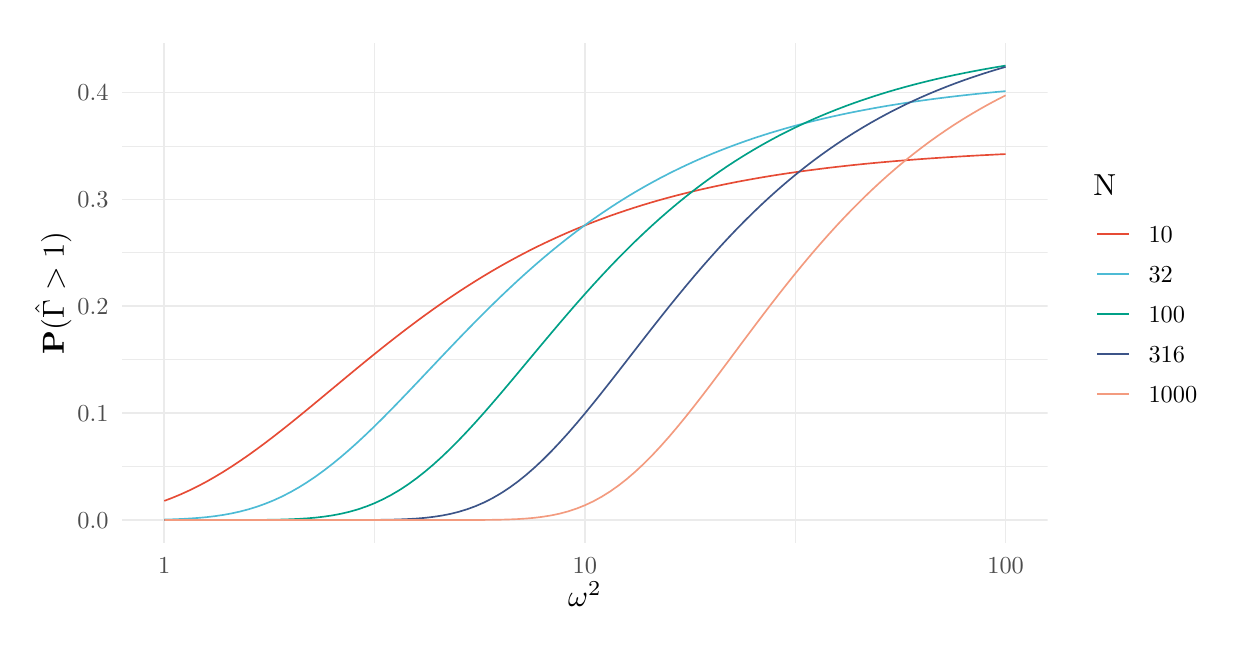
\begin{tikzpicture}[x=1pt,y=1pt]
\definecolor{fillColor}{RGB}{255,255,255}
\path[use as bounding box,fill=fillColor,fill opacity=0.00] (0,0) rectangle (433.62,216.81);
\begin{scope}
\path[clip] ( 34.16, 30.69) rectangle (368.57,211.31);
\definecolor{drawColor}{gray}{0.92}

\path[draw=drawColor,line width= 0.3pt,line join=round] ( 34.16, 58.20) --
	(368.57, 58.20);

\path[draw=drawColor,line width= 0.3pt,line join=round] ( 34.16, 96.82) --
	(368.57, 96.82);

\path[draw=drawColor,line width= 0.3pt,line join=round] ( 34.16,135.43) --
	(368.57,135.43);

\path[draw=drawColor,line width= 0.3pt,line join=round] ( 34.16,174.05) --
	(368.57,174.05);

\path[draw=drawColor,line width= 0.3pt,line join=round] (125.36, 30.69) --
	(125.36,211.31);

\path[draw=drawColor,line width= 0.3pt,line join=round] (277.37, 30.69) --
	(277.37,211.31);

\path[draw=drawColor,line width= 0.6pt,line join=round] ( 34.16, 38.90) --
	(368.57, 38.90);

\path[draw=drawColor,line width= 0.6pt,line join=round] ( 34.16, 77.51) --
	(368.57, 77.51);

\path[draw=drawColor,line width= 0.6pt,line join=round] ( 34.16,116.13) --
	(368.57,116.13);

\path[draw=drawColor,line width= 0.6pt,line join=round] ( 34.16,154.74) --
	(368.57,154.74);

\path[draw=drawColor,line width= 0.6pt,line join=round] ( 34.16,193.35) --
	(368.57,193.35);

\path[draw=drawColor,line width= 0.6pt,line join=round] ( 49.36, 30.69) --
	( 49.36,211.31);

\path[draw=drawColor,line width= 0.6pt,line join=round] (201.36, 30.69) --
	(201.36,211.31);

\path[draw=drawColor,line width= 0.6pt,line join=round] (353.37, 30.69) --
	(353.37,211.31);
\definecolor{drawColor}{RGB}{230,75,53}

\path[draw=drawColor,line width= 0.6pt,line join=round] ( 49.36, 45.81) --
	( 52.40, 46.97) --
	( 55.44, 48.24) --
	( 58.48, 49.62) --
	( 61.52, 51.12) --
	( 64.56, 52.73) --
	( 67.60, 54.46) --
	( 70.64, 56.28) --
	( 73.68, 58.21) --
	( 76.72, 60.23) --
	( 79.76, 62.33) --
	( 82.80, 64.52) --
	( 85.84, 66.77) --
	( 88.88, 69.09) --
	( 91.92, 71.46) --
	( 94.96, 73.88) --
	( 98.00, 76.34) --
	(101.04, 78.83) --
	(104.08, 81.34) --
	(107.12, 83.86) --
	(110.16, 86.39) --
	(113.20, 88.92) --
	(116.24, 91.44) --
	(119.28, 93.95) --
	(122.32, 96.44) --
	(125.36, 98.90) --
	(128.40,101.34) --
	(131.44,103.74) --
	(134.48,106.10) --
	(137.52,108.43) --
	(140.56,110.71) --
	(143.60,112.94) --
	(146.64,115.12) --
	(149.68,117.26) --
	(152.72,119.34) --
	(155.76,121.37) --
	(158.80,123.34) --
	(161.84,125.26) --
	(164.88,127.13) --
	(167.92,128.94) --
	(170.96,130.70) --
	(174.00,132.40) --
	(177.04,134.04) --
	(180.08,135.64) --
	(183.12,137.18) --
	(186.16,138.67) --
	(189.20,140.10) --
	(192.24,141.49) --
	(195.28,142.83) --
	(198.32,144.12) --
	(201.36,145.36) --
	(204.40,146.56) --
	(207.44,147.71) --
	(210.48,148.82) --
	(213.52,149.88) --
	(216.56,150.91) --
	(219.60,151.89) --
	(222.64,152.84) --
	(225.68,153.75) --
	(228.72,154.62) --
	(231.76,155.46) --
	(234.80,156.26) --
	(237.84,157.03) --
	(240.88,157.77) --
	(243.92,158.48) --
	(246.97,159.16) --
	(250.01,159.81) --
	(253.05,160.44) --
	(256.09,161.04) --
	(259.13,161.61) --
	(262.17,162.16) --
	(265.21,162.69) --
	(268.25,163.20) --
	(271.29,163.68) --
	(274.33,164.14) --
	(277.37,164.58) --
	(280.41,165.01) --
	(283.45,165.41) --
	(286.49,165.80) --
	(289.53,166.18) --
	(292.57,166.53) --
	(295.61,166.87) --
	(298.65,167.20) --
	(301.69,167.51) --
	(304.73,167.81) --
	(307.77,168.09) --
	(310.81,168.36) --
	(313.85,168.62) --
	(316.89,168.87) --
	(319.93,169.11) --
	(322.97,169.34) --
	(326.01,169.56) --
	(329.05,169.76) --
	(332.09,169.96) --
	(335.13,170.15) --
	(338.17,170.34) --
	(341.21,170.51) --
	(344.25,170.68) --
	(347.29,170.83) --
	(350.33,170.99) --
	(353.37,171.13);
\definecolor{drawColor}{RGB}{77,187,213}

\path[draw=drawColor,line width= 0.6pt,line join=round] ( 49.36, 39.07) --
	( 52.40, 39.15) --
	( 55.44, 39.27) --
	( 58.48, 39.44) --
	( 61.52, 39.65) --
	( 64.56, 39.93) --
	( 67.60, 40.29) --
	( 70.64, 40.74) --
	( 73.68, 41.29) --
	( 76.72, 41.96) --
	( 79.76, 42.76) --
	( 82.80, 43.69) --
	( 85.84, 44.78) --
	( 88.88, 46.01) --
	( 91.92, 47.41) --
	( 94.96, 48.97) --
	( 98.00, 50.70) --
	(101.04, 52.59) --
	(104.08, 54.64) --
	(107.12, 56.85) --
	(110.16, 59.20) --
	(113.20, 61.69) --
	(116.24, 64.31) --
	(119.28, 67.04) --
	(122.32, 69.88) --
	(125.36, 72.81) --
	(128.40, 75.82) --
	(131.44, 78.90) --
	(134.48, 82.03) --
	(137.52, 85.20) --
	(140.56, 88.39) --
	(143.60, 91.61) --
	(146.64, 94.82) --
	(149.68, 98.04) --
	(152.72,101.23) --
	(155.76,104.41) --
	(158.80,107.55) --
	(161.84,110.65) --
	(164.88,113.71) --
	(167.92,116.71) --
	(170.96,119.66) --
	(174.00,122.55) --
	(177.04,125.38) --
	(180.08,128.14) --
	(183.12,130.83) --
	(186.16,133.45) --
	(189.20,136.00) --
	(192.24,138.47) --
	(195.28,140.87) --
	(198.32,143.20) --
	(201.36,145.45) --
	(204.40,147.63) --
	(207.44,149.74) --
	(210.48,151.77) --
	(213.52,153.74) --
	(216.56,155.63) --
	(219.60,157.46) --
	(222.64,159.22) --
	(225.68,160.91) --
	(228.72,162.55) --
	(231.76,164.11) --
	(234.80,165.62) --
	(237.84,167.07) --
	(240.88,168.47) --
	(243.92,169.81) --
	(246.97,171.09) --
	(250.01,172.32) --
	(253.05,173.51) --
	(256.09,174.64) --
	(259.13,175.73) --
	(262.17,176.78) --
	(265.21,177.78) --
	(268.25,178.74) --
	(271.29,179.65) --
	(274.33,180.54) --
	(277.37,181.38) --
	(280.41,182.19) --
	(283.45,182.96) --
	(286.49,183.70) --
	(289.53,184.41) --
	(292.57,185.09) --
	(295.61,185.74) --
	(298.65,186.36) --
	(301.69,186.95) --
	(304.73,187.52) --
	(307.77,188.07) --
	(310.81,188.59) --
	(313.85,189.08) --
	(316.89,189.56) --
	(319.93,190.02) --
	(322.97,190.45) --
	(326.01,190.87) --
	(329.05,191.27) --
	(332.09,191.65) --
	(335.13,192.01) --
	(338.17,192.36) --
	(341.21,192.69) --
	(344.25,193.01) --
	(347.29,193.31) --
	(350.33,193.60) --
	(353.37,193.88);
\definecolor{drawColor}{RGB}{0,160,135}

\path[draw=drawColor,line width= 0.6pt,line join=round] ( 49.36, 38.90) --
	( 52.40, 38.90) --
	( 55.44, 38.90) --
	( 58.48, 38.90) --
	( 61.52, 38.90) --
	( 64.56, 38.90) --
	( 67.60, 38.90) --
	( 70.64, 38.90) --
	( 73.68, 38.90) --
	( 76.72, 38.91) --
	( 79.76, 38.92) --
	( 82.80, 38.93) --
	( 85.84, 38.96) --
	( 88.88, 39.00) --
	( 91.92, 39.07) --
	( 94.96, 39.17) --
	( 98.00, 39.31) --
	(101.04, 39.51) --
	(104.08, 39.77) --
	(107.12, 40.13) --
	(110.16, 40.58) --
	(113.20, 41.16) --
	(116.24, 41.87) --
	(119.28, 42.74) --
	(122.32, 43.77) --
	(125.36, 44.99) --
	(128.40, 46.40) --
	(131.44, 48.00) --
	(134.48, 49.80) --
	(137.52, 51.81) --
	(140.56, 54.01) --
	(143.60, 56.41) --
	(146.64, 58.99) --
	(149.68, 61.75) --
	(152.72, 64.66) --
	(155.76, 67.73) --
	(158.80, 70.92) --
	(161.84, 74.23) --
	(164.88, 77.63) --
	(167.92, 81.12) --
	(170.96, 84.67) --
	(174.00, 88.27) --
	(177.04, 91.90) --
	(180.08, 95.55) --
	(183.12, 99.20) --
	(186.16,102.84) --
	(189.20,106.46) --
	(192.24,110.05) --
	(195.28,113.60) --
	(198.32,117.10) --
	(201.36,120.53) --
	(204.40,123.91) --
	(207.44,127.21) --
	(210.48,130.45) --
	(213.52,133.60) --
	(216.56,136.67) --
	(219.60,139.66) --
	(222.64,142.56) --
	(225.68,145.38) --
	(228.72,148.11) --
	(231.76,150.75) --
	(234.80,153.31) --
	(237.84,155.78) --
	(240.88,158.17) --
	(243.92,160.47) --
	(246.97,162.69) --
	(250.01,164.83) --
	(253.05,166.89) --
	(256.09,168.87) --
	(259.13,170.77) --
	(262.17,172.60) --
	(265.21,174.36) --
	(268.25,176.05) --
	(271.29,177.68) --
	(274.33,179.24) --
	(277.37,180.73) --
	(280.41,182.16) --
	(283.45,183.54) --
	(286.49,184.86) --
	(289.53,186.12) --
	(292.57,187.33) --
	(295.61,188.49) --
	(298.65,189.60) --
	(301.69,190.66) --
	(304.73,191.68) --
	(307.77,192.65) --
	(310.81,193.59) --
	(313.85,194.48) --
	(316.89,195.33) --
	(319.93,196.15) --
	(322.97,196.93) --
	(326.01,197.68) --
	(329.05,198.40) --
	(332.09,199.08) --
	(335.13,199.74) --
	(338.17,200.36) --
	(341.21,200.96) --
	(344.25,201.53) --
	(347.29,202.08) --
	(350.33,202.60) --
	(353.37,203.10);
\definecolor{drawColor}{RGB}{60,84,136}

\path[draw=drawColor,line width= 0.6pt,line join=round] ( 49.36, 38.90) --
	( 52.40, 38.90) --
	( 55.44, 38.90) --
	( 58.48, 38.90) --
	( 61.52, 38.90) --
	( 64.56, 38.90) --
	( 67.60, 38.90) --
	( 70.64, 38.90) --
	( 73.68, 38.90) --
	( 76.72, 38.90) --
	( 79.76, 38.90) --
	( 82.80, 38.90) --
	( 85.84, 38.90) --
	( 88.88, 38.90) --
	( 91.92, 38.90) --
	( 94.96, 38.90) --
	( 98.00, 38.90) --
	(101.04, 38.90) --
	(104.08, 38.90) --
	(107.12, 38.90) --
	(110.16, 38.90) --
	(113.20, 38.90) --
	(116.24, 38.90) --
	(119.28, 38.91) --
	(122.32, 38.92) --
	(125.36, 38.94) --
	(128.40, 38.98) --
	(131.44, 39.03) --
	(134.48, 39.12) --
	(137.52, 39.25) --
	(140.56, 39.43) --
	(143.60, 39.69) --
	(146.64, 40.05) --
	(149.68, 40.51) --
	(152.72, 41.11) --
	(155.76, 41.87) --
	(158.80, 42.79) --
	(161.84, 43.91) --
	(164.88, 45.23) --
	(167.92, 46.77) --
	(170.96, 48.53) --
	(174.00, 50.52) --
	(177.04, 52.73) --
	(180.08, 55.17) --
	(183.12, 57.82) --
	(186.16, 60.67) --
	(189.20, 63.71) --
	(192.24, 66.93) --
	(195.28, 70.29) --
	(198.32, 73.80) --
	(201.36, 77.42) --
	(204.40, 81.14) --
	(207.44, 84.94) --
	(210.48, 88.79) --
	(213.52, 92.68) --
	(216.56, 96.60) --
	(219.60,100.52) --
	(222.64,104.44) --
	(225.68,108.33) --
	(228.72,112.18) --
	(231.76,116.00) --
	(234.80,119.75) --
	(237.84,123.44) --
	(240.88,127.06) --
	(243.92,130.60) --
	(246.97,134.06) --
	(250.01,137.44) --
	(253.05,140.72) --
	(256.09,143.91) --
	(259.13,147.01) --
	(262.17,150.01) --
	(265.21,152.92) --
	(268.25,155.73) --
	(271.29,158.45) --
	(274.33,161.07) --
	(277.37,163.60) --
	(280.41,166.04) --
	(283.45,168.39) --
	(286.49,170.65) --
	(289.53,172.82) --
	(292.57,174.91) --
	(295.61,176.92) --
	(298.65,178.85) --
	(301.69,180.70) --
	(304.73,182.48) --
	(307.77,184.18) --
	(310.81,185.82) --
	(313.85,187.39) --
	(316.89,188.89) --
	(319.93,190.33) --
	(322.97,191.71) --
	(326.01,193.03) --
	(329.05,194.29) --
	(332.09,195.50) --
	(335.13,196.66) --
	(338.17,197.77) --
	(341.21,198.83) --
	(344.25,199.85) --
	(347.29,200.82) --
	(350.33,201.75) --
	(353.37,202.64);
\definecolor{drawColor}{RGB}{243,155,127}

\path[draw=drawColor,line width= 0.6pt,line join=round] ( 49.36, 38.90) --
	( 52.40, 38.90) --
	( 55.44, 38.90) --
	( 58.48, 38.90) --
	( 61.52, 38.90) --
	( 64.56, 38.90) --
	( 67.60, 38.90) --
	( 70.64, 38.90) --
	( 73.68, 38.90) --
	( 76.72, 38.90) --
	( 79.76, 38.90) --
	( 82.80, 38.90) --
	( 85.84, 38.90) --
	( 88.88, 38.90) --
	( 91.92, 38.90) --
	( 94.96, 38.90) --
	( 98.00, 38.90) --
	(101.04, 38.90) --
	(104.08, 38.90) --
	(107.12, 38.90) --
	(110.16, 38.90) --
	(113.20, 38.90) --
	(116.24, 38.90) --
	(119.28, 38.90) --
	(122.32, 38.90) --
	(125.36, 38.90) --
	(128.40, 38.90) --
	(131.44, 38.90) --
	(134.48, 38.90) --
	(137.52, 38.90) --
	(140.56, 38.90) --
	(143.60, 38.90) --
	(146.64, 38.90) --
	(149.68, 38.90) --
	(152.72, 38.90) --
	(155.76, 38.90) --
	(158.80, 38.91) --
	(161.84, 38.92) --
	(164.88, 38.93) --
	(167.92, 38.97) --
	(170.96, 39.02) --
	(174.00, 39.11) --
	(177.04, 39.24) --
	(180.08, 39.43) --
	(183.12, 39.70) --
	(186.16, 40.08) --
	(189.20, 40.57) --
	(192.24, 41.21) --
	(195.28, 42.02) --
	(198.32, 43.02) --
	(201.36, 44.23) --
	(204.40, 45.66) --
	(207.44, 47.33) --
	(210.48, 49.23) --
	(213.52, 51.38) --
	(216.56, 53.77) --
	(219.60, 56.40) --
	(222.64, 59.24) --
	(225.68, 62.30) --
	(228.72, 65.56) --
	(231.76, 68.98) --
	(234.80, 72.57) --
	(237.84, 76.29) --
	(240.88, 80.12) --
	(243.92, 84.04) --
	(246.97, 88.03) --
	(250.01, 92.07) --
	(253.05, 96.14) --
	(256.09,100.23) --
	(259.13,104.31) --
	(262.17,108.36) --
	(265.21,112.39) --
	(268.25,116.37) --
	(271.29,120.30) --
	(274.33,124.15) --
	(277.37,127.94) --
	(280.41,131.64) --
	(283.45,135.26) --
	(286.49,138.78) --
	(289.53,142.21) --
	(292.57,145.55) --
	(295.61,148.78) --
	(298.65,151.91) --
	(301.69,154.95) --
	(304.73,157.88) --
	(307.77,160.71) --
	(310.81,163.45) --
	(313.85,166.08) --
	(316.89,168.62) --
	(319.93,171.06) --
	(322.97,173.42) --
	(326.01,175.68) --
	(329.05,177.85) --
	(332.09,179.93) --
	(335.13,181.94) --
	(338.17,183.86) --
	(341.21,185.70) --
	(344.25,187.47) --
	(347.29,189.17) --
	(350.33,190.79) --
	(353.37,192.35);
\end{scope}
\begin{scope}
\path[clip] (  0.00,  0.00) rectangle (433.62,216.81);
\definecolor{drawColor}{gray}{0.30}

\node[text=drawColor,anchor=base east,inner sep=0pt, outer sep=0pt, scale=  0.88] at ( 29.21, 35.87) {0.0};

\node[text=drawColor,anchor=base east,inner sep=0pt, outer sep=0pt, scale=  0.88] at ( 29.21, 74.48) {0.1};

\node[text=drawColor,anchor=base east,inner sep=0pt, outer sep=0pt, scale=  0.88] at ( 29.21,113.09) {0.2};

\node[text=drawColor,anchor=base east,inner sep=0pt, outer sep=0pt, scale=  0.88] at ( 29.21,151.71) {0.3};

\node[text=drawColor,anchor=base east,inner sep=0pt, outer sep=0pt, scale=  0.88] at ( 29.21,190.32) {0.4};
\end{scope}
\begin{scope}
\path[clip] (  0.00,  0.00) rectangle (433.62,216.81);
\definecolor{drawColor}{gray}{0.30}

\node[text=drawColor,anchor=base,inner sep=0pt, outer sep=0pt, scale=  0.88] at ( 49.36, 19.68) {1};

\node[text=drawColor,anchor=base,inner sep=0pt, outer sep=0pt, scale=  0.88] at (201.36, 19.68) {10};

\node[text=drawColor,anchor=base,inner sep=0pt, outer sep=0pt, scale=  0.88] at (353.37, 19.68) {100};
\end{scope}
\begin{scope}
\path[clip] (  0.00,  0.00) rectangle (433.62,216.81);
\definecolor{drawColor}{RGB}{0,0,0}

\node[text=drawColor,anchor=base,inner sep=0pt, outer sep=0pt, scale=  1.10] at (201.36,  7.64) {$\omega^2$};
\end{scope}
\begin{scope}
\path[clip] (  0.00,  0.00) rectangle (433.62,216.81);
\definecolor{drawColor}{RGB}{0,0,0}

\node[text=drawColor,rotate= 90.00,anchor=base,inner sep=0pt, outer sep=0pt, scale=  1.10] at ( 13.08,121.00) {$\mathbf P ( \hat \Gamma > 1 )$};
\end{scope}
\begin{scope}
\path[clip] (  0.00,  0.00) rectangle (433.62,216.81);
\definecolor{drawColor}{RGB}{0,0,0}

\node[text=drawColor,anchor=base west,inner sep=0pt, outer sep=0pt, scale=  1.10] at (385.07,156.09) {N};
\end{scope}
\begin{scope}
\path[clip] (  0.00,  0.00) rectangle (433.62,216.81);
\definecolor{drawColor}{RGB}{230,75,53}

\path[draw=drawColor,line width= 0.6pt,line join=round] (386.52,142.30) -- (398.08,142.30);
\end{scope}
\begin{scope}
\path[clip] (  0.00,  0.00) rectangle (433.62,216.81);
\definecolor{drawColor}{RGB}{77,187,213}

\path[draw=drawColor,line width= 0.6pt,line join=round] (386.52,127.84) -- (398.08,127.84);
\end{scope}
\begin{scope}
\path[clip] (  0.00,  0.00) rectangle (433.62,216.81);
\definecolor{drawColor}{RGB}{0,160,135}

\path[draw=drawColor,line width= 0.6pt,line join=round] (386.52,113.39) -- (398.08,113.39);
\end{scope}
\begin{scope}
\path[clip] (  0.00,  0.00) rectangle (433.62,216.81);
\definecolor{drawColor}{RGB}{60,84,136}

\path[draw=drawColor,line width= 0.6pt,line join=round] (386.52, 98.94) -- (398.08, 98.94);
\end{scope}
\begin{scope}
\path[clip] (  0.00,  0.00) rectangle (433.62,216.81);
\definecolor{drawColor}{RGB}{243,155,127}

\path[draw=drawColor,line width= 0.6pt,line join=round] (386.52, 84.48) -- (398.08, 84.48);
\end{scope}
\begin{scope}
\path[clip] (  0.00,  0.00) rectangle (433.62,216.81);
\definecolor{drawColor}{RGB}{0,0,0}

\node[text=drawColor,anchor=base west,inner sep=0pt, outer sep=0pt, scale=  0.88] at (405.02,139.27) {10};
\end{scope}
\begin{scope}
\path[clip] (  0.00,  0.00) rectangle (433.62,216.81);
\definecolor{drawColor}{RGB}{0,0,0}

\node[text=drawColor,anchor=base west,inner sep=0pt, outer sep=0pt, scale=  0.88] at (405.02,124.81) {32};
\end{scope}
\begin{scope}
\path[clip] (  0.00,  0.00) rectangle (433.62,216.81);
\definecolor{drawColor}{RGB}{0,0,0}

\node[text=drawColor,anchor=base west,inner sep=0pt, outer sep=0pt, scale=  0.88] at (405.02,110.36) {100};
\end{scope}
\begin{scope}
\path[clip] (  0.00,  0.00) rectangle (433.62,216.81);
\definecolor{drawColor}{RGB}{0,0,0}

\node[text=drawColor,anchor=base west,inner sep=0pt, outer sep=0pt, scale=  0.88] at (405.02, 95.91) {316};
\end{scope}
\begin{scope}
\path[clip] (  0.00,  0.00) rectangle (433.62,216.81);
\definecolor{drawColor}{RGB}{0,0,0}

\node[text=drawColor,anchor=base west,inner sep=0pt, outer sep=0pt, scale=  0.88] at (405.02, 81.45) {1000};
\end{scope}
\end{tikzpicture}
%
    }
    \caption{
        We show the probability that the estimated posterior variance $\hat \Gamma$ is bigger than the prior variance $1$ when varying the noise variance $\omega^{2}$. {\textcolor{red} todo: ausführlicher beschreiben} %
        % for small N: N / N-1 difference in estimation
        % as omega grows, prob. increases
        % as N increases, larger omega necessary
    }
    \label{fig:ce_prob_failure}
\end{figure}

% all of these even worse if dimension grows
In higher-dimensional settings, e.g. when applying the \gls{cem} to \glspl{ssm}, we expect this phenomenon to occur even more often. In the extreme case of independent marginals, i.e. when $\Sigma$ is a diagonal matrix, \Cref{eq:gamma_post} reduces to $(n + 1)p$ many decoupled equations, where $\hat \Gamma_{i,i}, i =1, \dots, (n + 1)p$ are independent. If all $q_{i} = \P \left(\Gamma_{i,i} > \Sigma_{i,i}\right)$ are identical to $q \in (0, 1)$, e.g. because $\Sigma$ and $\Omega$ are multiples of the identity, the number of failures follows a $\operatorname{Binom} \left( (n + 1)p, q \right)$ distribution, so that even small $q$ may lead to a non-negligible number of failures. 

If we admit noise variance $\infty$ in our optimization, then $\Gamma > 1$ implies that the \gls{cem} chooses this as the estimate, i.e. $\G_{\psi}$ is $\mathcal N(0, 1)$, which is equal to the prior. We can interpret this as having a missing observation, which, going back to the \gls{ssm} context, the Kalman-filter \Cref{alg:kalman_filter} can handle with only simple modifications, see e.g. \cite[Section 4.10]{Durbin2012Time}. However, if there are a lot of failures, the optimally chosen $\G_{\hpce}$ will still be close to the prior distribution of states $X$, and importance sampling is unlikely to be effective. 

%% Markov works better

\begin{tcolorbox}[title={Decide whether to keep and where to move}]
    
In this section, we analyze the properties of Gaussian proposals for importance sampling in \glspl{ssm} that exploit the available Markov property of states. As mentioned in the introduction to this section, these proposals are conditional distributions $\P^{X|Z=z}$ where $ \mathbf{R}^{m} \ni X \sim \mathcal N \left( \mu, \Sigma \right)$ and $Z = BX + \eta \in \mathbf{R}^{p}$ where $\eta\sim\mathcal N(0, \Omega)$ is independent of $X$. Standard results from linear regression theory imply that the conditional distribution in question is again a Gaussian distribution, $X|Z=z \sim \mathcal N(\bar \mu, \bar \Sigma)$ with mean
\begin{align}
    \bar \mu    & = \mu + \Sigma B^{T} \left( B \Sigma B^{T} + \Omega \right)^{-1} (z - B \mu), \label{eq:posterior_mean_1} \\
                & = \bar \Sigma\left(\Sigma^{-1}\mu + B^{T}\Omega^{-1}z \right)\label{eq:posterior_mean_2}                  \\
    \intertext{and covariance matrix}
    \bar \Sigma & = \Sigma - \Sigma B^T \left( B\Sigma B^{T} + \Omega \right) ^{-1} B \Sigma \label{eq:posterior_cov_1}     \\
                & = \left(\Sigma^{-1} + B^{T}\Omega^{-1}B\right)^{-1} \label{eq:posterior_cov_2}.
\end{align}
Note that \Cref{eq:posterior_mean_1,eq:posterior_cov_1} are more general, requiring only $B \Sigma B + \Omega$ be invertible, while the others require both $\Sigma$ and $\Omega$ to be invertible, see \cite[Lemma 7.1]{Chopin2020Introduction} for further discussion.

\end{tcolorbox}

\begin{tcolorbox}[title={decide what to do}]
    
\subsection{Analysis of optimal parameters}
\label{subsec:analysis_of_optimal_parameters}


\begin{theorem}[Optimal EIS proposal]
    \label{thm:optimal-eis}
    Let $p(x)$ be some density and consider importance sampling by exponential family proposals with densities $$q_\psi(x) = h(x) \exp\left( \langle \psi,S(x)\rangle - A(\psi)\right)$$ with natural parameter $\psi \in \mathbf{R}^{k}$, base measure $h$, sufficient statistic $S$ and log-partition function $A$. The parameter $\hat \psi$ that minimizes the variance of log importance sampling weights $\log w_{\psi}(x) = \log p(x) - \log q_{\psi}(x)$ is given by
    \begin{align*}
        \hat \psi & =  \argmin _{\psi} \var \left( \log w_{\psi}(X) \right)        \\
                  & = \cov(S(X))^{-1}\cov\left(S(X), \log \frac{p(X)}{h(X)}\right)
    \end{align*}
    where $X \sim p$.
\end{theorem}
\begin{proof}
    \todo{formultae this, consider exact assumptions}
\end{proof}

\begin{remark}[Optimal Gaussian proposal]
    As the family of Gaussian distributions $\mathcal N \left( \mu, \Sigma \right)$ form an exponential family with natural parameter $\psi = \left( \Sigma ^{-1} \mu, -\frac{1}{2}\Sigma^{-1} \right)$ and sufficient statistic $S(x) = \left( x, x x^{T} \right)$, \Cref{thm:optimal-eis} implies that the optimal EIS Gaussian proposal involves up to fourth order moments of $p$.

    As a consequence we expect EIS to produce proposals that are more robust to skewness and heavier than Gaussian tails than the Laplace approximation \todo{which is validated by simulations in section ...}.
\end{remark}

\subsection{Analysis of convergence (?)}
\label{subsec:analysis-of-convergence}

Additionally, each iteration of the CE and EIS method may be seen as performing M-estimation and as such the one step estimates $\psi_{CE}$ and $\psi_{EIS}$ are, in the limit as the number of samples $M$ goes to $\infty$, asymptotically normally distributed.

Analyzing the multi-step behavior of these iterative estimates is more complex, as we want to keep a fixed seed, i.e. common random numbers, to ensure numerical convergence. Thus the distribution of the second iterate conditional on the first iterate depends only \todo{check} the conditional distribution of the common random numbers given the first iterate, which is intractable.

\begin{theorem}[Consistency of importance sampling estimates]
    \todo{apply van der vaart}
\end{theorem}

\begin{theorem}[Asymptotic normality of importance sampling estimates]
    \todo{calculate asymptotic covariances}
\end{theorem}
\begin{proof}
    \todo{all iterative procedures are M-estimators, so a single step is (in the limit of samples $N\to\infty$), under some regularity conditions, asymptotically normal, compare asymptotic variances}
\end{proof}

\todo{interpret this in a sensible way, probably EIS more numerically stable}
\end{tcolorbox}

%
\section{Accouting for multimodality and heavy tails}
\label{sec:accouting_for_multimodality_and_heavy_tails}
Performing importance sampling with the Gaussian models discussed so far will work well only if the smoothing distribution  $p(x|y)$ is well approximated by a Gaussian distribution. However, a Gaussian distribution is a very specific kind of distribution, in particular, it is an unimodal distribution
%that is constant on elliptical contours 
and has light tails \todo{check for correct wording}.

If the smoothing distribution violates any of these assumptions, importance sampling with the models presented so far is likely to fail, i.e. requiring large sample sizes for both finding the optimal importance sampling parameter $\hat \psi$ as well as the final importance sampling evaluation.

There are however techniques to keep most of the computational efficiency discussed in the above sections to address both multimodality as well as heavy tails.

We start with heavier than gaussian tails: the textbook example of a heavy tailed distribution is the multivariate $t$-distribution with density
$$
    \dots .
$$
for degrees of freedom  $\nu > 1$ \todo{?}, location $\mu$ and scale matrix $\Sigma$. When $\nu > 2$ then this distribution has mean $\mu$ and if $\nu > 3$ it has covariance matrix $?$ \todo{check}.

The main properties necessary to facilitate Gaussian importance sampling strategies above are that the distribution $p(x|y)$ is analytically tractable and simulation from it is possible. These properties still hold for the multivariate $t$-distribution and, in fact, for the even larger class of elliptical distributions:

\begin{theorem}[Conditional distribution of elliptical distributions]
    \label{thm:elliptical-conditional}
    \todo{cite the correct book}
\end{theorem}

As one can readily see from \Cref{thm:elliptical-conditional} the parameters of the smoothing distribution $p(x|y)$ if $p(x,y)$ follows an elliptical distribution is again elliptical and its parameters only depend on quantities that are computed by the Kalman smoother. \todo{elaborate}

\todo{present some models with heavy tails}


\section{Maximum likelihood estimation in SSMs}
\label{sec:maximum_likelihood_estimation}

% region introduction
%% need for MLE: hyperparameters
Until now, we have assumed that the \acrshort{ssm} under consideration is completely known, i.e. we have access to the true transition and observation kernels. For the models considered in this thesis (\Cref{cha:analysis_of_selected_models}), this is unrealistic, as they are not based on concrete physical processes but are rather statistical approximations of the true underlying dynamics. The transition densities of, e.g., \Cref{eq:glssm_states} will depend on the covariance matrix of innovations, of which we have no a priori knowledge and for negative binomially distributed observations the overdispersion parameter $r$ will be unknown. Let us denote by $\theta\in\R^{l}$ the vector of these hyperparameters. \todo{check l / k with psis}
To make this dependence explicit, we will introduce subscripts $\theta$ where appropriate, i.e. $\P_{\theta}$ is a target distribution that additionally depends on $\theta$, $p_{\theta}$ its density et cetera. This section is loosely based on \citep[Chapter 7 \& 11]{Durbin2012Time} and \citep[Chapter 14]{Chopin2020Introduction}

To determine a suitable value of $\theta$, multiple options are available. Here, we opt for a frequentist approach, using maximum likelihood estimation to determine an optimal $\hat \theta$. Therefore, given observations $y\in\R^{(n+1)\times p}$, $\hat\theta$ maximizes the likelihood $p_{\theta}(y)$ and can be obtained as the global maximum of the following optimization problem: 
$$
    \max_{\theta \in \Theta} p_{\theta}(y).
$$
For numerical stability, we should maximize the log-likelihood instead, i.e. solve 
\begin{align}
    \label{eq:max-log-p}
    \max_{\theta \in \Theta} \log p_{\theta}(y).
\end{align}
Here $\Theta \subseteq \R^{l}$ is the parameter space. To solve this optimization problem using gradient ascent algorithms, we need access to both the likelihood and its derivatives. Thus, in the following, we will assume that $\theta \mapsto \log p_{\theta}(y)$ is sufficiently smooth, to apply these methods, i.e. it has continuous derivatives of second order. 

%% GLSSM analytically available, still need to use gradient descent algs. 
%% analytically impossible
%% high dimensional integral -> importance sampling
While the Kalman-filter (\Cref{alg:kalman_filter}) allows analytical computation of this likelihood \acrshortpl{glssm}, in general \acrshortpl{ssm} it is numerically intractable. The reason for this is that
$$
    p_{\theta}(y) = \int p_{\theta}(x,y) \mathrm d \mu(x)
$$
is a high-dimensional integral, which is hard to evaluate numerically. Instead, we will use importance sampling to estimate the likelihood. For this, let us regard $p_{\theta}(x,y)$ as an unnormalized density in $x$. The missing integration constant is then just $p_{\theta}(y)$ and the normalized density is $p_{\theta}(x|y)$. If $\G \gg \P$ is a proposal distribution whose density $g$ with respect to $\mu$ we can evaluate analytically, i.e. not only up to a constant, we see that for the unnormalized weights $\tilde w_{\theta}(x) = \frac{p_{\theta}(x,y)}{g(x)}$, that $p_{\theta}(y) = \G [\tilde w_{\theta}]$. Thus we may estimate the likelihood by 
$$
    \verywidehat{p_{\theta}(y)} = \frac{1}{N}\sum_{i = 1}^N \tilde w_{\theta} (X^{i})
$$
for $X^{1}, \dots, X^{N} \iid \G$ and $N \in \N$. To evaluate the gradient, notice that as $\nabla_{\theta} p_{\theta}(x,y) = p_{\theta}(x,y) \nabla_{\theta} \log p_{\theta}(x,y)$, we have, provided we can exchange integration and differentiation,
\begin{align*}
     \nabla_{\theta} p_{\theta}(y) &= \nabla_{\theta}\int p_{\theta}(x,y)\d \mu(x) = \int p_{\theta}(x,y) \nabla_{\theta} \log p_{\theta}(x,y)\d \mu(x) \\
     &= \G [\tilde w_{\theta} \nabla_{\theta} \log p_{\theta}(x,y)],
\end{align*}
and so we may estimate the gradient by 
\begin{align*}
    \verywidehat{\nabla_{\theta} p_{\theta}(y)} &= \frac{1}{N}\sum_{i = 1}^N \tilde w_{\theta}(X^{i}) \nabla_{\theta} \log p_{\theta}(X^{i}, y)
    %&= \sum_{i = 1}^N \tilde w_{\theta}(X^{i}) \sum_{t = 0}^n \nabla_{\theta} \left( \log p_{\theta}(y_{t} | X^{i}_{t}) + \log p_{\theta}(X^{i}_t|X^{i}_{t - 1}) \right).
\end{align*}
Similarly, we can estimate the log-likelihood by Plug-In
\begin{align}
    \label{eq:loglik-hat-standard}
    \verywidehat{\log p_{\theta}(y)} = \log \left( \frac{1}{N}\sum_{i = 1}^N \tilde w_{\theta}(X^{i}) \right)
\end{align}
and its gradient, using the fact that the gradient of $\log f$ for $f: \R^{l} \to \R$ is $ \frac{1}{f} \nabla_{\theta} f$, by 
\begin{align*}
    \verywidehat{\nabla_{\theta} \log p_{\theta}(y)} &= \left(\frac{1}{N} \sum_{i = 1}^N \tilde w_{\theta}(X^{i}) \right)^{-1} \left( \frac{1}{N}\sum_{i = 1}^N \tilde w_{\theta}(X^{i}) \nabla_{\theta} \log p_{\theta}(X^{i}, y) \right) \\
    &=\sum_{i = 1}^N W_{\theta}^{i} \nabla_{\theta} \log p_{\theta}(X^{i}, y)
\end{align*}
where $W_{\theta}^{i} = \frac{\tilde w_{\theta}(X^{i})}{\sum_{i= 1}^N \tilde w_{\theta}(X^{i})}$ are the auto-normalized weights.
Note that, by Jensen's inequality, these estimates are biased.


%% optimizatino using CRNs, advantage over particle filters
To solve the optimization problem \eqref{eq:max-log-p} we will again employ \acrshortpl{crn}. If the densities involved are twice differentiable, this device ensures that the random objective function $\theta \mapsto \sum_{i = 1}^N \tilde w_{\theta}(X^{i})$ is twice differentiable, and so we can indeed apply gradient ascent to find a local maximum. This is an advantage of performing global importance sampling over \acrshort{smc}, i.e. particle filter, methods. To avoid collapse to a single particle, \acrshort{smc} methods perform intermediate resampling steps, which make the objective function discontinuous. While particle smoothing methods can mitigate this problem, they are more expensive than standard \acrshort{smc} and, as the importance sampling estimates of the log-likelihood and its gradient are biased, the usual requirements for stochastic approximation methods are not fulfilled. 
For a more thorough discussion of the challenges maximum likelihood estimation with \acrshort{smc} methods faces, we recommend \citep[Chapter 14]{Chopin2020Introduction}.

%% discuss not really frequentist setting
While \acrshortpl{mle} have a strong frequentist foundation, let us stress that, for the models that we investigate in \Cref{cha:analysis_of_selected_models}, the frequentist properties of the estimates are not of interest. The reason for this is that a frequentist interpretation requires us to imagine, at least hypothetically, an infinite repetition of the data-generating process. For the data at hand, such repetition is nonsensical: the pandemic is a \glqq{}one-off\grqq{} event that will not be replicated under even approximately similar circumstances. Therefore, we will choose to view the estimation procedure more as a hyper-parameter tuning step, rather than true frequentist inference. While we can compute asymptotic confidence intervals for $\hat\theta$, see, e.g., \citep[Chapter 11.6]{Durbin2012Time}, \citep[Chapter 14.8]{Chopin2020Introduction}, these are not of practical interest for similar reasons. 

%% alternative: fully Bayesian
As an alternative to modeling $\theta$ as fixed, but unknown, and performing maximum-likelihood estimation to obtain $\hat \theta$, one might also model $\theta$ as random with prior density $p(\theta)$, such that the full model becomes $p(x,y,\theta) = p(x,y|\theta)p(\theta)$. In this setup, sometimes called the Bayesian treatment of \acrshortpl{ssm} \citep[Section 13.1]{Durbin2012Time}, the main interest still lies in the posterior density $p(x,\theta|y)$, which, depending on the model at hand, can drastically increase the difficulty of the problem: even if $p(x,y|\theta)$ is an analytically tractable model such as a \acrshort{glssm}, unless the prior is chosen to be conjugate, one has to resort to, e.g., \acrshort{mcmc}-methods. 

% endregion

% region GLSSM proposal

%% joint density easy to calculate
By the structure of the model, \Cref{eq:joint_density}, the log density and its gradient can be computed efficiently by
\begin{align*}
    \log p_{\theta}(x,y) &= \log p_{\theta}(x_{0}) + \sum_{t = 1}^{n} \log p_{\theta}(x_{t}|x_{t-1}) + \log p_{\theta} (y_{t}|x_{t},y_{t - 1})\\
    \nabla_{\theta}\log p_{\theta}(x,y) &= \nabla_{\theta}\log p_{\theta}(x_{0}) + \sum_{t = 1}^{n} \nabla_{\theta}\log p_{\theta}(x_{t}|x_{t-1}) + \nabla_{\theta}\log p_{\theta} (y_{t}|x_{t},y_{t - 1}),
\end{align*}
respectively. 

Similarly, when proposing with a \acrshort{glssm} or Markov-proposal for a \acrshort{pgssm}, the weights have similar structure, see\Cref{eq:weights_markov,eq:weights_only_on_signal}, which makes calculation of $\tilde w$ efficient. 

For the remainder of this section, let us consider the \acrshort{glssm}-proposal obtained by \acrshort{eis} for a \acrshort{pgssm} with linear signal, as this is the main setting of \Cref{cha:analysis_of_selected_models}. For this we obtain 
$$
    \tilde w_{\theta}(x) = \tilde w_{\theta}(s) g(z)\frac{p_{\theta}(y|s)}{g(z|s)} = g(z) \prod_{t = 0}^n \frac{p_{\theta}(y_{t}|s_{t})}{g(z_{t}|s_{t})},
$$
where $s_{t} = B_{t}x_{t}$, $t = 0, \dots, n$, is the signal, and so the log-likelihood is given by 
\begin{align}
    \label{eq:loglik-pgssm-exact}
    \log p_{\theta}(y) = \log g_{\theta}(z) + \log \E \left(w_{\theta}(S)|Y = y\right)
\end{align}
and can be estimated by
\begin{align}
    \label{eq:loglik-hat-linearsignal}
    \verywidehat{\log p_{\theta}(y)} = \log g_{\theta}(z) + \log \left(\frac{1}{N}\sum_{i=1}^{N}\prod_{t = 0}^{n} \frac{p_{\theta}(y_{t}|S^{i}_{t})}{ g(z_{t}|S^{i}_{t})}\right).
\end{align}
Notice that $\log g_{\theta}(z)$ is the likelihood in a \acrshort{glssm}, which can be computed efficiently by the standard Kalman filter (\Cref{alg:kalman_filter}). As in the \acrshort{glssm}-approach we propose with an \acrshort{glssm} whose state density $g(x)$ and observation matrices $B_{t}$, $t = 0, \dots, n$ are equal to those of the target, the log-likelihood $\log g_{\theta}(z)$ also depends on $\theta$. The estimated gradient of the log-likelihood is 
$$
    \verywidehat{\nabla_{\theta} \log p_{\theta}(y)} = \nabla_{\theta} \log g_{\theta}(z) + \sum_{i=1}^N W^{i}_\theta \sum_{t = 0}^n \nabla_{\theta} \log p_{\theta}(y_{t}|S_{t}^{i}).
$$
The gradient of the \acrshort{glssm} log-likelihood can be obtained either numerically or analytically by employing the Kalman filter and smoother \citep{Koopman1992Exact}, however, numerical evaluation may be faster if the dimension of $\theta$ is small compared to the length of the time series, as evaluating the likelihood only requires a single application of the Kalman filter. 

As the observation densities $g(z_{t}|s_{t})$ do not depend on $\theta$, their derivatives do not appear in the above estimate. However, when using \acrshort{eis} to determine an optimal proposal, the parameter $\psi = (z, \omega)$ implicitly depends on $\theta$. Accounting for this yields the gradient 
$$
    \verywidehat{\nabla_{\theta} \log p_{\theta}(y)} = \nabla_{\theta} \log g_{\theta}(z) + \sum_{i=1}^N W^{i}_\theta \left(\sum_{t = 0}^n \nabla_{\theta} \log p_{\theta}(y_{t}|S_{t}^{i}) - \nabla_{\theta} \log g_{\theta}(z_{t}|S^{i}_{t})\right),
$$
as $\nabla_{\theta} \frac{1}{g_{\theta}(z|s)} = - \frac{1}{g_{\theta}(z|s)} \nabla_{\theta} \log g_{\theta}(z|s)$. The computation of this additional term is much more involved, as the parameters $z,\Omega$ are found through an iterative numerical scheme. Instead, we favor numerical differentiation of the whole procedure to evaluate the likelihood at $\theta$, including the method of finding an optimal importance sampling scheme. 


As a single evaluation of the log-likelihood can become very expensive we want our procedure to be as efficient as possible. To this end, \citep{Durbin1997Monte} provides several improvements to the basic algorithm if the model is a \acrshort{pgssm} with a linear signal. Their contributions consist of a bias correction for the log-likelihood, the use of antithetic and control variables to reduce Monte-Carlo error for importance sampling and a deterministic initialization procedure.
Let us briefly summarize these ideas, adapted to our notation. As the computational gains for control variates in the presence of antithetic variables seem to be limited, we do not give the same level of detail here, for an in-depth analysis, we refer the reader to the source. 

% bias reduction
For bias reduction, a second-order Taylor series expansion shows that for $\tilde{w}_\cdot = \frac{1}{N} \sum_{i =1}^N \tilde w(X^{i})$,
\begin{align*}
    \E \left(\log \tilde{w}_\cdot\right) - \log \G \tilde w &= \E \log \left(1 + \frac{\tilde{w}_\cdot - \G \tilde w}{\G \tilde w} \right)\\
                                                           &=  \frac{\tilde{w}_\cdot - \G \tilde w}{\G \tilde w}  - \frac{1}{2} \left(\frac{\tilde{w}_\cdot - \G \tilde w}{\G \tilde w} \right)^{2} + \mathcal O_{p}(N^{-\frac{3}{2}}),
\end{align*}
provided $\tilde w \in L^{3}(\G)$. Thus, estimating the second order term by $- \frac{\hat\sigma^2}{2N \tilde{w}_\cdot} $, where $\hat \sigma^{2}$ is the empirical variance of the unnormalized weights, we can perform a bias reduction by estimating 
\begin{align}
    \label{eq:loglik-hat-bias-reduction}
    \widehat{\log p_{\theta}(y)} = \log \left(\tilde w_{\cdot}\right) + \log g_{\theta}(z) + \frac{\hat\sigma^{2}}{2N\tilde w_{\cdot}}
\end{align}

% antithetics
The second improvement of \citep{Durbin1997Monte} is the use of antithetic variables and control variates, a device to reduce Monte-Carlo variance. The main idea of an antithetic variable is to construct for each sample $X^{i}$, $i = 1,\dots, N$, another sample $\tilde X^{i}$ that has the same distribution as $X^{i}$, but is negatively correlated with $X^{i}$. This has two effects: first of all, we increase the number of samples used for importance sampling and second, as the new samples are negatively correlated with the old samples, the Monte-Carlo variance is reduced. The computation of these samples is usually much faster than creating new samples, which requires the use of the expensive \acrshort{ffbs} or simulation smoother algorithms. 
\begin{definition}[antithetic variable]
    Let $X, \tilde X\in\R^{k}$ be two random variables with the same distribution, $\mathcal L (X) = \mathcal L(\tilde X)$ and $f: \R^{k} \to \R$. Then $\tilde X$ is called an antithetic variable of $X$ for $f$, if $\cov \left( f(\tilde X), f(X) \right) < 0$. If $k = 1$ and $f$ is the identity, we just say that $\tilde X$ is an antithetic variable of $X$.
\end{definition}

% location & scale
\citep{Durbin1997Monte} introduce two antithetic variables: balanced for location and balanced for scale, both of which are tailored to the multivariate normal distribution. 
\begin{definition}[antithetic variable balanced for location and scale, \citep{Durbin1997Monte}]
    Let $X\sim \mathcal N(\mu, \Sigma)$ for $\mu \in \R^{k}$ and $\Sigma \in \R^{k\times k}$ positive definite. We call
    \begin{align}
        \label{eq:antithetic-location}
    \tilde X = \mu + (\mu - X)
    \end{align}
    the antithetic balanced for location. If $L\in\R^{k\times k}$ is a Cholesky root of $\Sigma$ and 
    $$
        X = \mu + L \varepsilon
    $$
    with $\varepsilon \sim \mathcal N(0, I)$, let $c = \varepsilon^{T}\varepsilon \sim \chi^{2}_k$ and $c' = F^{-1}_{\chi^{2}_{k}}(1 - F_{\chi^{2}_k}(\sqrt{c}))$. We call
    \begin{align}
        \label{eq:antithetic-scale}
        \check X = \mu + \sqrt{\frac{c'}{c}} \left( X - \mu \right)
    \end{align}
    the antithetic balanced for location.
\end{definition}
\begin{lemma}
    In the above definition, $\tilde X_{i}$ is an antithetic variable of $X$ for the coordinate functions $f_{i}:\R^{k} \to \R$, $f_{i}(x) = x_{i}$, $i = 1, \dots, k$.
    Furthermore, $\tilde c$ is an antithetic variable of $c$.
\end{lemma}
\begin{proof}
    It is easy to see that $\tilde X$ has the same distribution as $X$. Furthermore 
    $$
        \cov \left( f_{i}(X), f_{i}(\tilde X)\right) = \cov \left( 2 \mu_{i} - X_{i}, X_{i} \right) = - \Sigma_{i,i} < 0.
    $$

    For $c$ and $\tilde c$, let $U = F_{\chi^{2}_{k}}(c)$, then $U \sim \operatorname{Unif}(0,1)$ and $\tilde U = 1 - U = F_{\chi^{2}_k}(\tilde c)$. 
    As $\tilde U \sim \operatorname{Unif}(0, 1)$ as well, $\mathcal L (c) = \mathcal L (\tilde c)$.
    In \citep[Lemma 2.3]{Whitt1976Bivariate} it is shown that for any pair of real-valued random variables $(Y,W)$ with CDF $H$ and marginal CDFs $F, G$, it holds
    $$
        \cov \left(Y,W \right) = \int_{\R^{2}} H(y,w) - F(y)G(w) \d y \d w,
    $$
    and, furthermore, by \citep[Theorem 2.1 and Lemma 2.4]{Whitt1976Bivariate} that the joint CDF of $(c, \tilde c)$ is $(y,w) \mapsto \max \{0, F(y) + G(w) - 1\}$, where $F$ is the CDF of $c$ and $G$ the CDF of $\tilde c$. 
    As 
    $$
        a + b - 1 = ab + a(1-b) + b - 1 = ab - (1 - a)(1 - b) < ab
    $$
    for all $a,b \in (0,1)$, we have 
    \begin{align*}
        \cov \left( c, \tilde c \right) &= \int_{\R^{2}} H(y,w) - F(y)G(w) \d y \d w \\
        &= \int_{\R^{2}} \max\{0, F(y) + G(w) - 1\} - F(y)G(w) \d y \d w < 0.
    \end{align*}
\end{proof}
Let us mention that, by the properties of the standard multivariate normal distribution, $ c = \lVert u \rVert $ and $ \frac{u}{ \lVert u \rVert }$ are independent. Writing 
$$
    X = \mu + \lVert u \rVert L \frac{u}{ \lVert u \rVert } = \mu + \lVert u \rVert \frac{X - \mu}{\sqrt{c}},
$$
we see that 
$$
    \check X = \mu + \sqrt{\tilde c}\frac{X - \mu}{\sqrt{c}}
$$
has the same distribution as $X$, as $\tilde c \sim \mathcal L( \lVert u \rVert^{2})$ and is independent of $ \frac{X - \mu}{\sqrt{c}}$. 

Given a \acrshort{glssm}-proposal and samples $X^{1}, \dots, X^{N}$ from it, we can cheaply calculate these antithetic variables: for the location balanced antithetic we can calculate the mean using the Kalman-smoother and for the scale balanced antithetic we can calculate $c$ and $c'$ using the inverse CDF of the $\chi^{2}_{k}$ distribution and the standard normal samples used to sample $X^{i}$ in the first place, for which fast implementations are readily available. Incidental, we obtain a third antithetic, 
\begin{align}
    \label{eq:antithetic-scale-location}
    \breve{X} = \mu - \sqrt{ \frac{c'}{c}} (X - \mu)
\end{align}
for free. We can then estimate the log-likelihood in \Cref{eq:loglik-hat-bias-reduction} by replacing each occurrence of $\tilde w_{\theta}(X^{i})$ by 
\begin{align}
    \label{eq:antithetic-weights}
    \frac{1}{4} \left( \tilde w_{\theta} (X^{i}) + \tilde w_{\theta}(\tilde{X^{i}}) + \tilde w_{\theta}(\check{X^{i}}) + \tilde w_{\theta}(\breve{{X^{i}}}) \right).
\end{align}



% intialization
As the procedure to evaluate the likelihood by importance sampling becomes expensive as the dimension of the model increases, \citep{Durbin1997Monte} recommend finding an initial value $\hat \theta_{0}$ by maximizing a deterministic version of \Cref{eq:loglik-hat-standard}. For this, denote by $s^{\ast}$ the mode of the linear signal, conditional on the pseudo-observations $z$. As $S$ follows a multivariate Gaussian, $s^{\ast}$ is also the mean which can be computed efficiently by the Kalman or signal-smoother. Approximating the conditional expectation in \Cref{eq:loglik-pgssm-exact} by $w_{\theta}(s^{\ast})$ then yields 
\begin{align}
    \label{eq:loglik-initial-approx-mode}
    \log p_{\theta}(y) \approx \log g_{\theta}(z) + \log w_{\theta}(s^{\ast}),
\end{align}
which can be evaluated without simulation by the \acrshort{la}. A better approximation can be obtained by performing a fourth-order Taylor expansion of $s\mapsto w_{\theta}(s)$ around the mode $s^\ast$, which yields 
\begin{align}
    \label{eq:loglik-initial-tayolor-approx-mode}
    \log p_{\theta}(y) \approx \log g_{\theta}(z) + \log w_{\theta}(s^{\ast}) + \log \left( 1 + \frac{1}{8} \sum_{t = 1}^n\sum_{j = 1}^m l^{(4)}_{t,j}(s^{\ast}) v_{t,j}^2 \right),
\end{align}
where $l^{(4)}$ is the fourth derivative of the log-weights $s\mapsto \log w_{\theta}(s)$ and $v_{t,j}$ is the conditional variance $\var \left( S_{t,j} | Z = z \right)$ in the proposal. Again, we refer the interested reader to the source for the details.

% endregion
\begin{algorithm}
    \label{alg:mle}
    \begin{algorithmic}[1]
        \Require parameterized \acrshort{pgssm} with linear signal, initial $\theta^{0} \in \Theta$, observations $y \in \R^{(n+1)p}$, number of samples $N$
        % initialization
        \Function{approx\_loglik}{$\theta$}
            \State obtain \acrshort{la} of the \acrshort{pgssm} for $\theta$ \Comment{\Cref{alg:la}}
            \State obtain mode $s^{\ast}$ and conditional variances $v_{t,j}$ from the \acrshort{la} \Comment{\Cref{alg:kalman_filter,alg:kalman_smoother}}
            \State \textbf{return} approximate log-likelihood \Comment{\Cref{eq:loglik-initial-approx-mode} or \Cref{eq:loglik-initial-tayolor-approx-mode}}
        \EndFunction 
        \Statex

        \Function{estimate\_loglik}{$\theta$}
            \State obtain \acrshort{la} of the \acrshort{pgssm} for $\theta$ \Comment{\Cref{alg:la}}
            \State obtain \acrshort{eis} proposal $\G_{(z,\Omega)}$ \Comment{\Cref{alg:eis}, \acrshort{la} as initial values}
            \State sample $N$ signals $S^{i}$ from $S|Z = z$ in \acrshort{eis} \Comment{\Cref{alg:ffbs} or signal smoother}
            \State obtain mode $s^{\ast}$ in \acrshort{eis} proposal \Comment{\Cref{alg:kalman_smoother} or signal smoother}
            \State calculate antithetic variables $\tilde{S^{i}},\check{S^{i}}, \breve{{S^{i}}}$ \Comment{\Cref{eq:antithetic-location,eq:antithetic-scale,eq:antithetic-scale-location}}
            \State set $\tilde w_{\theta}^i = \frac{1}{4} \left( \tilde w_{\theta} (X^{i}) + \tilde w_{\theta}(\tilde{X^{i}}) + \tilde w_{\theta}(\check{X^{i}}) + \tilde w_{\theta}(\breve{{X^{i}}}) \right)$ \Cref{eq:antithetic-weights}
            \State set $\tilde w_{\cdot} = \frac{1}{N}\sum_{i = 1}^N \tilde w^{i}_{\theta}$
            \State set $\hat \sigma^{2} = \frac{1}{N - 1} \sum_{i = 1}^N \left( \tilde w_{\theta}^{i} - \tilde w_{\cdot}\right)^{2}$
            \State calculate $\log g_{\theta}(z)$ \Comment{\Cref{alg:kalman_filter}}
            \State \textbf{return} $\verywidehat{\log p_{\theta}(y)}$ \Comment{\Cref{eq:loglik-hat-bias-reduction}}
        \EndFunction
        \Statex

        \State maximize \textrm{APPROX\_LOGLIK} with initial value $\theta^{0}$  \Comment{numerically}
        \State set $\theta^{0} $ to optimal value
        \State maximize \textrm{ESTIMATE\_LOGLIK} with initial value $\theta^{0}$ and \acrshortpl{crn}  \Comment{numerically}
        \State set $\hat \theta$ to optimal value
        \State \textbf{return} $\hat \theta $
    \end{algorithmic}
    \caption{Maximum likelihood estimation in a \acrshort{pgssm} with linear signal using \acrshort{eis}.}
\end{algorithm}

The resulting procedure to find the MLE $\hat \theta$ in a \acrshort{pgssm} with linear signal is summarized in \Cref{alg:mle}. Notice that we use \acrshortpl{crn} to ensure numerical convergence. The numerical optimization can be performed using any standard solver such as the BFGS algorithm \citep[Chapter 6.1]{Nocedal2006Numerical}. We cannot give guarantees that this procedure produces the true \acrshort{mle}, i.e. finds the global maximizer. However, as we have discussed earlier, we are not interested in frequentist properties of $\hat \theta$ but see the estimation procedure as a hyperparameter tuning step. Thus, a local maximum may well be sufficient. Nevertheless, checking different starting points and random number seeds should be used to get as close as possible to the global maximum.

% region outlook
Notice that our discussion implies that we cannot reuse a \acrshort{glssm} proposal used for $\theta$ at another $\theta'$, as $p_{\theta'}(x) \neq g_{\theta}(x)$. While we can still calculate the weights using the general \Cref{eq:loglik-hat-standard}, we presume that the old proposal is not a good choice for the new target. The reason for this is that $\theta$ will usually contain parameters related to the covariance structure of the innovations and observations, and these parameters usually affect many, if not all states or observations. For example, it is common to model states that perform a random walk with common innovation variance $\sigma^{2}$ as an element of $\theta$. As the distributions lie in a high-dimensional space, slight misspecification of the covariance structure will drastically deteriorate the performance of importance sampling. 

If computations are so involved that we want to avoid running the optimal importance sampling scheme as much as possible, one could try, if the model under investigation allows for it, to split $\theta$ into $(\theta_{x}, \theta_y)$ where $\theta_{x}$ only affects the state transitions and $\theta_{y}$ only affects the observation densities. Then a coordinate ascent scheme could be employed, where the update step for $\theta_{y}$ can reuse the proposal, provided that $\theta_{y}$ does not change too much and the observation density $p_{\theta}(y|x)$ is not too sensitive to changes in $\theta_{y}$, which should imply that the proposal is still close enough to give good importance sampling performance. Then numerical differentiation is only required to update $\theta_{x}$. 

% endregion

\section{Comparison of Importance Sampling method}
\label{sec:simulation_studies}

\begin{example}[univariate Gaussian, $\sigma^{2}$ fixed]
    \label{ex:univ-gaussian-s2-fixed}
    Consider the probability space $ \left( \R, \mathcal B(\R), \P \right)$ where $\P = p\lambda$ for the Lebesgue measure $\lambda$ which is symmetric around $0$, i.e. $p(-x) = p(x)$ for $\lambda$-a.e. $x\in\R$ and possesses up to third order moments.
    Let $\G=\P$, so $W\equiv1$ and let $\G_{\psi} = \mathcal N \left( \sigma\psi, \sigma^{2} \right)$ be the single parameter natural exponential family of Gaussians with fixed variance $\sigma^{2} > 0$. Then 
    $$
    \log g_{\psi}(x) = \psi T(x) - \frac{\psi^{2}}{2} + \log h(x),
    $$
    where $T(x) = \frac{x}{\sigma}$ and $h(x)$ is the density of $\mathcal N(0, \sigma^{2})$ w.r.t. Lebesgue measure. 
    Note that $T$ is centered under $\P$. To compare the asymptotic behavior of the \gls{cem} and \gls{eis} we compute the asymptotic variances arising from their respective central limit theorems (\Cref{thm:ce-clt,thm:clt-eis}).

    By symmetry, both $\pce$ and $\peis$ are equal to $0$. 
    Then $I(\psi) = 1$ for all $\psi$, so 
    \begin{align}
    \label{eq:ce-gaussian-mean-var}
        V_{\ce} = \cov_{\P}(T) = \frac{\tau^{2}}{\sigma^{2}},
    \end{align}
    where $\tau^{2}=\P \operatorname{id}^{2}$ is the second moment of $\P$. 
    Additionally, $B_{\eis} = (\cov_{\P}(T))^{-1} = \frac{\sigma^{2}}{\tau^{2}}$ and
    \begin{align*}
    M_{\eis} &= \cov_{\P} \left( (\log \frac{p(x)}{h(x)} - \lambda_{\eis})T\right) \\
        &= \cov_{\P} \left(\left( \log p - \log h - \P (\log p - \log h) \right) T \right) \\
        &= \frac{1}{\sigma^{2}}\int p(x) x^{2}\left(\log p(x) + \frac{x^{2}}{2\sigma^{2}} - \P\left(\log p(x) + \frac{\tau^{2}}{2\sigma^{2}}\right)\right)^{2} \d x.
    \end{align*}
    Thus
    $$
    V_{\eis} = B_{\eis}M_{\eis}B_{\eis}= \sigma^{2}\frac{\gamma}{\tau^{4}},
    $$
    where $\gamma = \int p(x) x^{2}\left(\log p(x) + \frac{x^{2}}{2\sigma^{2}} - \P(\log p(x) + \frac{\tau^{2}}{2\sigma^{2}})\right)^{2} \d x.$
    
    \paragraph{Normal distribution}
    If $\P = \mathcal N(0, \tau^{2})$ is a normal distribution, this reduces to
    \begin{align*}
        V_{\eis} &= \frac{5}{2} \left( \frac{\tau^{2}}{\sigma^{2}} - 1 \right)^{2} \frac{\sigma^{2}}{\tau^{2}} = \frac{5}{2} \frac{\left( V_{\ce} - 1\right)^{2}}{V_{\ce}}
    \end{align*}
    and so for $\tau^{2} = \sigma^{2}$ $\hpeis$ converges faster than the standard $\mathcal O( N^{-\frac{1}{2}})$ rate. Indeed in this case $\hpeis = \peis$ a.s. for $N > 1$ see \todo{write example for EIS being exact for exponential families}. 

    For importance sampling to be consistent, it is necessary that $\sigma^{2} > \frac{\tau^{2}}{2}$. The left-hand side of \Cref{fig:normal_are} displays the behavior of the relative efficiency
    $$
    \frac{V_{\eis}}{V_{\ce}} = \frac{5}{2} \frac{(V_{\ce} - 1)^{2}}{V_{\ce}^{2}} = \frac{5}{2} \left( 1 - \frac{2}{Vsdf_{\ce}} + \frac{1}{V_{\ce}^2} \right)
    $$

    \begin{figure}
        \centering

        \begin{subfigure}{.49\textwidth}
            \resizebox{\textwidth}{!}{%
                % Created by tikzDevice version 0.12.6 on 2024-06-05 16:48:21
% !TEX encoding = UTF-8 Unicode
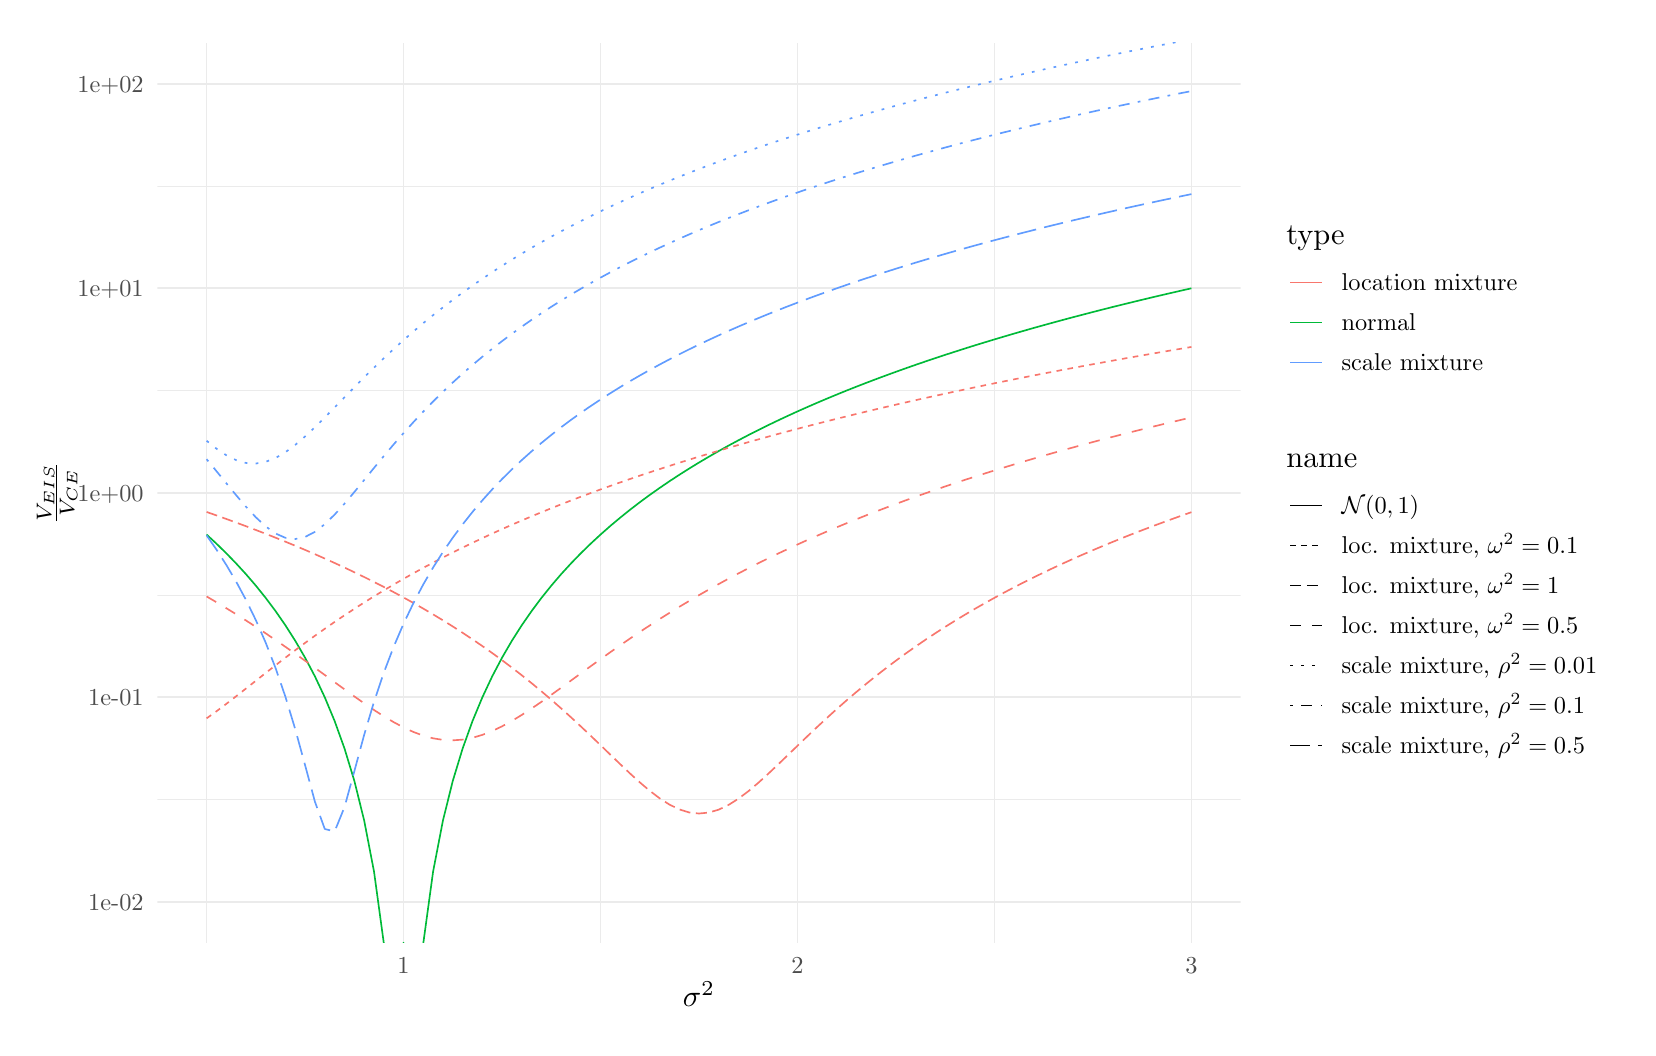
\begin{tikzpicture}[x=1pt,y=1pt]
\definecolor{fillColor}{RGB}{255,255,255}
\path[use as bounding box,fill=fillColor,fill opacity=0.00] (0,0) rectangle (578.16,361.35);
\begin{scope}
\path[clip] ( 46.86, 30.69) rectangle (438.30,355.85);
\definecolor{drawColor}{gray}{0.92}

\path[draw=drawColor,line width= 0.3pt,line join=round] ( 46.86, 82.42) --
	(438.30, 82.42);

\path[draw=drawColor,line width= 0.3pt,line join=round] ( 46.86,156.32) --
	(438.30,156.32);

\path[draw=drawColor,line width= 0.3pt,line join=round] ( 46.86,230.22) --
	(438.30,230.22);

\path[draw=drawColor,line width= 0.3pt,line join=round] ( 46.86,304.12) --
	(438.30,304.12);

\path[draw=drawColor,line width= 0.3pt,line join=round] ( 64.66, 30.69) --
	( 64.66,355.85);

\path[draw=drawColor,line width= 0.3pt,line join=round] (207.00, 30.69) --
	(207.00,355.85);

\path[draw=drawColor,line width= 0.3pt,line join=round] (349.34, 30.69) --
	(349.34,355.85);

\path[draw=drawColor,line width= 0.6pt,line join=round] ( 46.86, 45.47) --
	(438.30, 45.47);

\path[draw=drawColor,line width= 0.6pt,line join=round] ( 46.86,119.37) --
	(438.30,119.37);

\path[draw=drawColor,line width= 0.6pt,line join=round] ( 46.86,193.27) --
	(438.30,193.27);

\path[draw=drawColor,line width= 0.6pt,line join=round] ( 46.86,267.17) --
	(438.30,267.17);

\path[draw=drawColor,line width= 0.6pt,line join=round] ( 46.86,341.07) --
	(438.30,341.07);

\path[draw=drawColor,line width= 0.6pt,line join=round] (135.83, 30.69) --
	(135.83,355.85);

\path[draw=drawColor,line width= 0.6pt,line join=round] (278.17, 30.69) --
	(278.17,355.85);

\path[draw=drawColor,line width= 0.6pt,line join=round] (420.51, 30.69) --
	(420.51,355.85);
\definecolor{drawColor}{RGB}{0,186,56}

\path[draw=drawColor,line width= 0.6pt,line join=round] ( 64.66,178.18) --
	( 68.22,174.89) --
	( 71.77,171.42) --
	( 75.33,167.75) --
	( 78.89,163.86) --
	( 82.45,159.72) --
	( 86.01,155.29) --
	( 89.57,150.53) --
	( 93.13,145.39) --
	( 96.68,139.81) --
	(100.24,133.69) --
	(103.80,126.93) --
	(107.36,119.37) --
	(110.92,110.80) --
	(114.48,100.90) --
	(118.04, 89.20) --
	(121.59, 74.87) --
	(125.15, 56.41) --
	(128.71, 30.38) --
	(132.27,-14.11) --
	(135.83, 30.69) --
	(139.39,-14.11) --
	(142.94, 30.38) --
	(146.50, 56.41) --
	(150.06, 74.87) --
	(153.62, 89.20) --
	(157.18,100.90) --
	(160.74,110.80) --
	(164.30,119.37) --
	(167.85,126.93) --
	(171.41,133.69) --
	(174.97,139.81) --
	(178.53,145.39) --
	(182.09,150.53) --
	(185.65,155.29) --
	(189.21,159.72) --
	(192.76,163.86) --
	(196.32,167.75) --
	(199.88,171.42) --
	(203.44,174.89) --
	(207.00,178.18) --
	(210.56,181.32) --
	(214.12,184.30) --
	(217.67,187.15) --
	(221.23,189.89) --
	(224.79,192.51) --
	(228.35,195.02) --
	(231.91,197.45) --
	(235.47,199.78) --
	(239.03,202.03) --
	(242.58,204.21) --
	(246.14,206.31) --
	(249.70,208.35) --
	(253.26,210.33) --
	(256.82,212.24) --
	(260.38,214.10) --
	(263.94,215.91) --
	(267.49,217.67) --
	(271.05,219.38) --
	(274.61,221.05) --
	(278.17,222.68) --
	(281.73,224.26) --
	(285.29,225.81) --
	(288.85,227.32) --
	(292.40,228.79) --
	(295.96,230.24) --
	(299.52,231.65) --
	(303.08,233.03) --
	(306.64,234.38) --
	(310.20,235.70) --
	(313.75,237.00) --
	(317.31,238.27) --
	(320.87,239.52) --
	(324.43,240.74) --
	(327.99,241.94) --
	(331.55,243.12) --
	(335.11,244.27) --
	(338.66,245.41) --
	(342.22,246.53) --
	(345.78,247.62) --
	(349.34,248.70) --
	(352.90,249.76) --
	(356.46,250.81) --
	(360.02,251.83) --
	(363.57,252.85) --
	(367.13,253.84) --
	(370.69,254.82) --
	(374.25,255.79) --
	(377.81,256.74) --
	(381.37,257.67) --
	(384.93,258.60) --
	(388.48,259.51) --
	(392.04,260.41) --
	(395.60,261.29) --
	(399.16,262.16) --
	(402.72,263.03) --
	(406.28,263.88) --
	(409.84,264.72) --
	(413.39,265.54) --
	(416.95,266.36) --
	(420.51,267.17);
\definecolor{drawColor}{RGB}{248,118,109}

\path[draw=drawColor,line width= 0.6pt,dash pattern=on 2pt off 2pt ,line join=round] ( 64.66,111.77) --
	( 68.22,114.32) --
	( 71.77,117.00) --
	( 75.33,119.75) --
	( 78.89,122.55) --
	( 82.45,125.36) --
	( 86.01,128.17) --
	( 89.57,130.95) --
	( 93.13,133.69) --
	( 96.68,136.39) --
	(100.24,139.03) --
	(103.80,141.62) --
	(107.36,144.14) --
	(110.92,146.61) --
	(114.48,149.01) --
	(118.04,151.35) --
	(121.59,153.64) --
	(125.15,155.86) --
	(128.71,158.02) --
	(132.27,160.13) --
	(135.83,162.19) --
	(139.39,164.19) --
	(142.94,166.14) --
	(146.50,168.04) --
	(150.06,169.90) --
	(153.62,171.71) --
	(157.18,173.48) --
	(160.74,175.20) --
	(164.30,176.89) --
	(167.85,178.54) --
	(171.41,180.15) --
	(174.97,181.72) --
	(178.53,183.26) --
	(182.09,184.77) --
	(185.65,186.24) --
	(189.21,187.69) --
	(192.76,189.10) --
	(196.32,190.49) --
	(199.88,191.85) --
	(203.44,193.18) --
	(207.00,194.49) --
	(210.56,195.77) --
	(214.12,197.03) --
	(217.67,198.26) --
	(221.23,199.48) --
	(224.79,200.67) --
	(228.35,201.84) --
	(231.91,202.99) --
	(235.47,204.13) --
	(239.03,205.24) --
	(242.58,206.34) --
	(246.14,207.41) --
	(249.70,208.47) --
	(253.26,209.52) --
	(256.82,210.55) --
	(260.38,211.56) --
	(263.94,212.55) --
	(267.49,213.54) --
	(271.05,214.51) --
	(274.61,215.46) --
	(278.17,216.40) --
	(281.73,217.33) --
	(285.29,218.24) --
	(288.85,219.14) --
	(292.40,220.03) --
	(295.96,220.91) --
	(299.52,221.78) --
	(303.08,222.63) --
	(306.64,223.48) --
	(310.20,224.31) --
	(313.75,225.13) --
	(317.31,225.95) --
	(320.87,226.75) --
	(324.43,227.54) --
	(327.99,228.33) --
	(331.55,229.10) --
	(335.11,229.87) --
	(338.66,230.62) --
	(342.22,231.37) --
	(345.78,232.11) --
	(349.34,232.84) --
	(352.90,233.56) --
	(356.46,234.28) --
	(360.02,234.99) --
	(363.57,235.69) --
	(367.13,236.38) --
	(370.69,237.06) --
	(374.25,237.74) --
	(377.81,238.41) --
	(381.37,239.08) --
	(384.93,239.73) --
	(388.48,240.38) --
	(392.04,241.03) --
	(395.60,241.67) --
	(399.16,242.30) --
	(402.72,242.92) --
	(406.28,243.54) --
	(409.84,244.16) --
	(413.39,244.77) --
	(416.95,245.37) --
	(420.51,245.97);

\path[draw=drawColor,line width= 0.6pt,dash pattern=on 4pt off 2pt ,line join=round] ( 64.66,186.35) --
	( 68.22,185.10) --
	( 71.77,183.82) --
	( 75.33,182.52) --
	( 78.89,181.20) --
	( 82.45,179.84) --
	( 86.01,178.46) --
	( 89.57,177.05) --
	( 93.13,175.61) --
	( 96.68,174.14) --
	(100.24,172.64) --
	(103.80,171.10) --
	(107.36,169.52) --
	(110.92,167.91) --
	(114.48,166.26) --
	(118.04,164.57) --
	(121.59,162.84) --
	(125.15,161.06) --
	(128.71,159.24) --
	(132.27,157.37) --
	(135.83,155.44) --
	(139.39,153.47) --
	(142.94,151.43) --
	(146.50,149.34) --
	(150.06,147.19) --
	(153.62,144.97) --
	(157.18,142.68) --
	(160.74,140.32) --
	(164.30,137.89) --
	(167.85,135.38) --
	(171.41,132.79) --
	(174.97,130.11) --
	(178.53,127.35) --
	(182.09,124.49) --
	(185.65,121.54) --
	(189.21,118.50) --
	(192.76,115.37) --
	(196.32,112.16) --
	(199.88,108.86) --
	(203.44,105.49) --
	(207.00,102.08) --
	(210.56, 98.63) --
	(214.12, 95.21) --
	(217.67, 91.84) --
	(221.23, 88.61) --
	(224.79, 85.59) --
	(228.35, 82.89) --
	(231.91, 80.61) --
	(235.47, 78.87) --
	(239.03, 77.77) --
	(242.58, 77.38) --
	(246.14, 77.73) --
	(249.70, 78.78) --
	(253.26, 80.49) --
	(256.82, 82.73) --
	(260.38, 85.41) --
	(263.94, 88.42) --
	(267.49, 91.64) --
	(271.05, 95.00) --
	(274.61, 98.42) --
	(278.17,101.87) --
	(281.73,105.29) --
	(285.29,108.66) --
	(288.85,111.96) --
	(292.40,115.18) --
	(295.96,118.32) --
	(299.52,121.36) --
	(303.08,124.31) --
	(306.64,127.17) --
	(310.20,129.94) --
	(313.75,132.63) --
	(317.31,135.22) --
	(320.87,137.74) --
	(324.43,140.18) --
	(327.99,142.54) --
	(331.55,144.83) --
	(335.11,147.05) --
	(338.66,149.21) --
	(342.22,151.31) --
	(345.78,153.34) --
	(349.34,155.32) --
	(352.90,157.25) --
	(356.46,159.13) --
	(360.02,160.95) --
	(363.57,162.73) --
	(367.13,164.47) --
	(370.69,166.16) --
	(374.25,167.81) --
	(377.81,169.43) --
	(381.37,171.00) --
	(384.93,172.54) --
	(388.48,174.05) --
	(392.04,175.52) --
	(395.60,176.97) --
	(399.16,178.38) --
	(402.72,179.76) --
	(406.28,181.11) --
	(409.84,182.44) --
	(413.39,183.74) --
	(416.95,185.02) --
	(420.51,186.27);

\path[draw=drawColor,line width= 0.6pt,dash pattern=on 4pt off 4pt ,line join=round] ( 64.66,155.82) --
	( 68.22,153.73) --
	( 71.77,151.58) --
	( 75.33,149.39) --
	( 78.89,147.14) --
	( 82.45,144.83) --
	( 86.01,142.48) --
	( 89.57,140.08) --
	( 93.13,137.62) --
	( 96.68,135.13) --
	(100.24,132.59) --
	(103.80,130.03) --
	(107.36,127.44) --
	(110.92,124.84) --
	(114.48,122.26) --
	(118.04,119.70) --
	(121.59,117.20) --
	(125.15,114.79) --
	(128.71,112.50) --
	(132.27,110.39) --
	(135.83,108.49) --
	(139.39,106.85) --
	(142.94,105.53) --
	(146.50,104.56) --
	(150.06,103.99) --
	(153.62,103.83) --
	(157.18,104.08) --
	(160.74,104.75) --
	(164.30,105.80) --
	(167.85,107.19) --
	(171.41,108.89) --
	(174.97,110.84) --
	(178.53,113.00) --
	(182.09,115.32) --
	(185.65,117.75) --
	(189.21,120.27) --
	(192.76,122.83) --
	(196.32,125.42) --
	(199.88,128.02) --
	(203.44,130.60) --
	(207.00,133.16) --
	(210.56,135.69) --
	(214.12,138.18) --
	(217.67,140.62) --
	(221.23,143.01) --
	(224.79,145.35) --
	(228.35,147.65) --
	(231.91,149.88) --
	(235.47,152.07) --
	(239.03,154.20) --
	(242.58,156.29) --
	(246.14,158.32) --
	(249.70,160.30) --
	(253.26,162.24) --
	(256.82,164.13) --
	(260.38,165.98) --
	(263.94,167.78) --
	(267.49,169.54) --
	(271.05,171.26) --
	(274.61,172.94) --
	(278.17,174.59) --
	(281.73,176.20) --
	(285.29,177.77) --
	(288.85,179.31) --
	(292.40,180.82) --
	(295.96,182.30) --
	(299.52,183.74) --
	(303.08,185.16) --
	(306.64,186.55) --
	(310.20,187.91) --
	(313.75,189.25) --
	(317.31,190.56) --
	(320.87,191.85) --
	(324.43,193.11) --
	(327.99,194.35) --
	(331.55,195.57) --
	(335.11,196.76) --
	(338.66,197.94) --
	(342.22,199.10) --
	(345.78,200.23) --
	(349.34,201.35) --
	(352.90,202.45) --
	(356.46,203.53) --
	(360.02,204.60) --
	(363.57,205.65) --
	(367.13,206.68) --
	(370.69,207.70) --
	(374.25,208.70) --
	(377.81,209.68) --
	(381.37,210.66) --
	(384.93,211.62) --
	(388.48,212.56) --
	(392.04,213.49) --
	(395.60,214.41) --
	(399.16,215.32) --
	(402.72,216.21) --
	(406.28,217.09) --
	(409.84,217.96) --
	(413.39,218.82) --
	(416.95,219.67) --
	(420.51,220.51);
\definecolor{drawColor}{RGB}{97,156,255}

\path[draw=drawColor,line width= 0.6pt,dash pattern=on 1pt off 3pt ,line join=round] ( 64.66,212.08) --
	( 68.22,209.22) --
	( 71.77,206.84) --
	( 75.33,205.08) --
	( 78.89,204.06) --
	( 82.45,203.85) --
	( 86.01,204.47) --
	( 89.57,205.86) --
	( 93.13,207.94) --
	( 96.68,210.57) --
	(100.24,213.63) --
	(103.80,216.97) --
	(107.36,220.50) --
	(110.92,224.13) --
	(114.48,227.78) --
	(118.04,231.42) --
	(121.59,235.00) --
	(125.15,238.50) --
	(128.71,241.92) --
	(132.27,245.24) --
	(135.83,248.45) --
	(139.39,251.56) --
	(142.94,254.57) --
	(146.50,257.47) --
	(150.06,260.28) --
	(153.62,263.00) --
	(157.18,265.62) --
	(160.74,268.16) --
	(164.30,270.61) --
	(167.85,272.99) --
	(171.41,275.30) --
	(174.97,277.53) --
	(178.53,279.70) --
	(182.09,281.80) --
	(185.65,283.84) --
	(189.21,285.83) --
	(192.76,287.76) --
	(196.32,289.64) --
	(199.88,291.47) --
	(203.44,293.25) --
	(207.00,294.98) --
	(210.56,296.68) --
	(214.12,298.33) --
	(217.67,299.94) --
	(221.23,301.52) --
	(224.79,303.06) --
	(228.35,304.56) --
	(231.91,306.04) --
	(235.47,307.48) --
	(239.03,308.89) --
	(242.58,310.27) --
	(246.14,311.62) --
	(249.70,312.95) --
	(253.26,314.25) --
	(256.82,315.53) --
	(260.38,316.78) --
	(263.94,318.01) --
	(267.49,319.21) --
	(271.05,320.40) --
	(274.61,321.56) --
	(278.17,322.70) --
	(281.73,323.83) --
	(285.29,324.93) --
	(288.85,326.02) --
	(292.40,327.09) --
	(295.96,328.14) --
	(299.52,329.17) --
	(303.08,330.19) --
	(306.64,331.19) --
	(310.20,332.18) --
	(313.75,333.16) --
	(317.31,334.12) --
	(320.87,335.06) --
	(324.43,335.99) --
	(327.99,336.91) --
	(331.55,337.82) --
	(335.11,338.71) --
	(338.66,339.59) --
	(342.22,340.46) --
	(345.78,341.32) --
	(349.34,342.17) --
	(352.90,343.00) --
	(356.46,343.83) --
	(360.02,344.64) --
	(363.57,345.45) --
	(367.13,346.25) --
	(370.69,347.03) --
	(374.25,347.81) --
	(377.81,348.57) --
	(381.37,349.33) --
	(384.93,350.08) --
	(388.48,350.82) --
	(392.04,351.56) --
	(395.60,352.28) --
	(399.16,353.00) --
	(402.72,353.70) --
	(406.28,354.41) --
	(409.84,355.10) --
	(413.39,355.78) --
	(416.95,356.46) --
	(420.51,357.14);

\path[draw=drawColor,line width= 0.6pt,dash pattern=on 1pt off 3pt on 4pt off 3pt ,line join=round] ( 64.66,205.42) --
	( 68.22,201.09) --
	( 71.77,196.73) --
	( 75.33,192.41) --
	( 78.89,188.25) --
	( 82.45,184.42) --
	( 86.01,181.12) --
	( 89.57,178.57) --
	( 93.13,177.01) --
	( 96.68,176.57) --
	(100.24,177.32) --
	(103.80,179.17) --
	(107.36,181.93) --
	(110.92,185.40) --
	(114.48,189.34) --
	(118.04,193.55) --
	(121.59,197.89) --
	(125.15,202.26) --
	(128.71,206.57) --
	(132.27,210.78) --
	(135.83,214.87) --
	(139.39,218.81) --
	(142.94,222.61) --
	(146.50,226.26) --
	(150.06,229.77) --
	(153.62,233.13) --
	(157.18,236.36) --
	(160.74,239.46) --
	(164.30,242.44) --
	(167.85,245.31) --
	(171.41,248.07) --
	(174.97,250.73) --
	(178.53,253.30) --
	(182.09,255.78) --
	(185.65,258.17) --
	(189.21,260.49) --
	(192.76,262.73) --
	(196.32,264.90) --
	(199.88,267.00) --
	(203.44,269.04) --
	(207.00,271.02) --
	(210.56,272.95) --
	(214.12,274.82) --
	(217.67,276.64) --
	(221.23,278.42) --
	(224.79,280.14) --
	(228.35,281.83) --
	(231.91,283.47) --
	(235.47,285.07) --
	(239.03,286.64) --
	(242.58,288.17) --
	(246.14,289.67) --
	(249.70,291.13) --
	(253.26,292.56) --
	(256.82,293.96) --
	(260.38,295.33) --
	(263.94,296.67) --
	(267.49,297.99) --
	(271.05,299.28) --
	(274.61,300.55) --
	(278.17,301.79) --
	(281.73,303.01) --
	(285.29,304.20) --
	(288.85,305.38) --
	(292.40,306.53) --
	(295.96,307.66) --
	(299.52,308.78) --
	(303.08,309.88) --
	(306.64,310.95) --
	(310.20,312.01) --
	(313.75,313.06) --
	(317.31,314.08) --
	(320.87,315.10) --
	(324.43,316.09) --
	(327.99,317.07) --
	(331.55,318.04) --
	(335.11,318.99) --
	(338.66,319.93) --
	(342.22,320.85) --
	(345.78,321.76) --
	(349.34,322.66) --
	(352.90,323.55) --
	(356.46,324.42) --
	(360.02,325.29) --
	(363.57,326.14) --
	(367.13,326.98) --
	(370.69,327.81) --
	(374.25,328.63) --
	(377.81,329.44) --
	(381.37,330.24) --
	(384.93,331.03) --
	(388.48,331.81) --
	(392.04,332.58) --
	(395.60,333.34) --
	(399.16,334.09) --
	(402.72,334.84) --
	(406.28,335.57) --
	(409.84,336.30) --
	(413.39,337.02) --
	(416.95,337.73) --
	(420.51,338.43);

\path[draw=drawColor,line width= 0.6pt,dash pattern=on 7pt off 3pt ,line join=round] ( 64.66,177.88) --
	( 68.22,172.76) --
	( 71.77,167.22) --
	( 75.33,161.19) --
	( 78.89,154.57) --
	( 82.45,147.26) --
	( 86.01,139.11) --
	( 89.57,129.95) --
	( 93.13,119.59) --
	( 96.68,107.86) --
	(100.24, 94.86) --
	(103.80, 81.65) --
	(107.36, 71.79) --
	(110.92, 70.91) --
	(114.48, 79.67) --
	(118.04, 92.66) --
	(121.59,105.81) --
	(125.15,117.76) --
	(128.71,128.34) --
	(132.27,137.68) --
	(135.83,145.99) --
	(139.39,153.42) --
	(142.94,160.15) --
	(146.50,166.27) --
	(150.06,171.89) --
	(153.62,177.07) --
	(157.18,181.87) --
	(160.74,186.36) --
	(164.30,190.55) --
	(167.85,194.50) --
	(171.41,198.22) --
	(174.97,201.74) --
	(178.53,205.08) --
	(182.09,208.26) --
	(185.65,211.29) --
	(189.21,214.18) --
	(192.76,216.96) --
	(196.32,219.61) --
	(199.88,222.17) --
	(203.44,224.62) --
	(207.00,226.99) --
	(210.56,229.27) --
	(214.12,231.48) --
	(217.67,233.61) --
	(221.23,235.67) --
	(224.79,237.67) --
	(228.35,239.61) --
	(231.91,241.50) --
	(235.47,243.33) --
	(239.03,245.11) --
	(242.58,246.84) --
	(246.14,248.52) --
	(249.70,250.17) --
	(253.26,251.77) --
	(256.82,253.33) --
	(260.38,254.86) --
	(263.94,256.35) --
	(267.49,257.81) --
	(271.05,259.23) --
	(274.61,260.63) --
	(278.17,261.99) --
	(281.73,263.33) --
	(285.29,264.64) --
	(288.85,265.92) --
	(292.40,267.18) --
	(295.96,268.41) --
	(299.52,269.62) --
	(303.08,270.81) --
	(306.64,271.98) --
	(310.20,273.12) --
	(313.75,274.25) --
	(317.31,275.35) --
	(320.87,276.44) --
	(324.43,277.51) --
	(327.99,278.56) --
	(331.55,279.60) --
	(335.11,280.62) --
	(338.66,281.62) --
	(342.22,282.61) --
	(345.78,283.58) --
	(349.34,284.54) --
	(352.90,285.48) --
	(356.46,286.41) --
	(360.02,287.33) --
	(363.57,288.23) --
	(367.13,289.13) --
	(370.69,290.01) --
	(374.25,290.87) --
	(377.81,291.73) --
	(381.37,292.57) --
	(384.93,293.41) --
	(388.48,294.23) --
	(392.04,295.04) --
	(395.60,295.85) --
	(399.16,296.64) --
	(402.72,297.42) --
	(406.28,298.19) --
	(409.84,298.96) --
	(413.39,299.71) --
	(416.95,300.46) --
	(420.51,301.20);
\end{scope}
\begin{scope}
\path[clip] (  0.00,  0.00) rectangle (578.16,361.35);
\definecolor{drawColor}{gray}{0.30}

\node[text=drawColor,anchor=base east,inner sep=0pt, outer sep=0pt, scale=  0.88] at ( 41.91, 42.44) {1e-02};

\node[text=drawColor,anchor=base east,inner sep=0pt, outer sep=0pt, scale=  0.88] at ( 41.91,116.34) {1e-01};

\node[text=drawColor,anchor=base east,inner sep=0pt, outer sep=0pt, scale=  0.88] at ( 41.91,190.24) {1e+00};

\node[text=drawColor,anchor=base east,inner sep=0pt, outer sep=0pt, scale=  0.88] at ( 41.91,264.14) {1e+01};

\node[text=drawColor,anchor=base east,inner sep=0pt, outer sep=0pt, scale=  0.88] at ( 41.91,338.04) {1e+02};
\end{scope}
\begin{scope}
\path[clip] (  0.00,  0.00) rectangle (578.16,361.35);
\definecolor{drawColor}{gray}{0.30}

\node[text=drawColor,anchor=base,inner sep=0pt, outer sep=0pt, scale=  0.88] at (135.83, 19.68) {1};

\node[text=drawColor,anchor=base,inner sep=0pt, outer sep=0pt, scale=  0.88] at (278.17, 19.68) {2};

\node[text=drawColor,anchor=base,inner sep=0pt, outer sep=0pt, scale=  0.88] at (420.51, 19.68) {3};
\end{scope}
\begin{scope}
\path[clip] (  0.00,  0.00) rectangle (578.16,361.35);
\definecolor{drawColor}{RGB}{0,0,0}

\node[text=drawColor,anchor=base,inner sep=0pt, outer sep=0pt, scale=  1.10] at (242.58,  7.64) {$\sigma^2$};
\end{scope}
\begin{scope}
\path[clip] (  0.00,  0.00) rectangle (578.16,361.35);
\definecolor{drawColor}{RGB}{0,0,0}

\node[text=drawColor,rotate= 90.00,anchor=base,inner sep=0pt, outer sep=0pt, scale=  1.10] at ( 13.08,193.27) {$\frac{V_{EIS}}{V_{CE}}$};
\end{scope}
\begin{scope}
\path[clip] (  0.00,  0.00) rectangle (578.16,361.35);
\definecolor{drawColor}{RGB}{0,0,0}

\node[text=drawColor,anchor=base west,inner sep=0pt, outer sep=0pt, scale=  1.10] at (454.80,283.11) {type};
\end{scope}
\begin{scope}
\path[clip] (  0.00,  0.00) rectangle (578.16,361.35);
\definecolor{drawColor}{RGB}{248,118,109}

\path[draw=drawColor,line width= 0.6pt,line join=round] (456.25,269.31) -- (467.81,269.31);
\end{scope}
\begin{scope}
\path[clip] (  0.00,  0.00) rectangle (578.16,361.35);
\definecolor{drawColor}{RGB}{0,186,56}

\path[draw=drawColor,line width= 0.6pt,line join=round] (456.25,254.86) -- (467.81,254.86);
\end{scope}
\begin{scope}
\path[clip] (  0.00,  0.00) rectangle (578.16,361.35);
\definecolor{drawColor}{RGB}{97,156,255}

\path[draw=drawColor,line width= 0.6pt,line join=round] (456.25,240.40) -- (467.81,240.40);
\end{scope}
\begin{scope}
\path[clip] (  0.00,  0.00) rectangle (578.16,361.35);
\definecolor{drawColor}{RGB}{0,0,0}

\node[text=drawColor,anchor=base west,inner sep=0pt, outer sep=0pt, scale=  0.88] at (474.76,266.28) {location mixture};
\end{scope}
\begin{scope}
\path[clip] (  0.00,  0.00) rectangle (578.16,361.35);
\definecolor{drawColor}{RGB}{0,0,0}

\node[text=drawColor,anchor=base west,inner sep=0pt, outer sep=0pt, scale=  0.88] at (474.76,251.83) {normal};
\end{scope}
\begin{scope}
\path[clip] (  0.00,  0.00) rectangle (578.16,361.35);
\definecolor{drawColor}{RGB}{0,0,0}

\node[text=drawColor,anchor=base west,inner sep=0pt, outer sep=0pt, scale=  0.88] at (474.76,237.37) {scale mixture};
\end{scope}
\begin{scope}
\path[clip] (  0.00,  0.00) rectangle (578.16,361.35);
\definecolor{drawColor}{RGB}{0,0,0}

\node[text=drawColor,anchor=base west,inner sep=0pt, outer sep=0pt, scale=  1.10] at (454.80,202.53) {name};
\end{scope}
\begin{scope}
\path[clip] (  0.00,  0.00) rectangle (578.16,361.35);
\definecolor{drawColor}{RGB}{0,0,0}

\path[draw=drawColor,line width= 0.6pt,line join=round] (456.25,188.73) -- (467.81,188.73);
\end{scope}
\begin{scope}
\path[clip] (  0.00,  0.00) rectangle (578.16,361.35);
\definecolor{drawColor}{RGB}{0,0,0}

\path[draw=drawColor,line width= 0.6pt,dash pattern=on 2pt off 2pt ,line join=round] (456.25,174.28) -- (467.81,174.28);
\end{scope}
\begin{scope}
\path[clip] (  0.00,  0.00) rectangle (578.16,361.35);
\definecolor{drawColor}{RGB}{0,0,0}

\path[draw=drawColor,line width= 0.6pt,dash pattern=on 4pt off 2pt ,line join=round] (456.25,159.83) -- (467.81,159.83);
\end{scope}
\begin{scope}
\path[clip] (  0.00,  0.00) rectangle (578.16,361.35);
\definecolor{drawColor}{RGB}{0,0,0}

\path[draw=drawColor,line width= 0.6pt,dash pattern=on 4pt off 4pt ,line join=round] (456.25,145.37) -- (467.81,145.37);
\end{scope}
\begin{scope}
\path[clip] (  0.00,  0.00) rectangle (578.16,361.35);
\definecolor{drawColor}{RGB}{0,0,0}

\path[draw=drawColor,line width= 0.6pt,dash pattern=on 1pt off 3pt ,line join=round] (456.25,130.92) -- (467.81,130.92);
\end{scope}
\begin{scope}
\path[clip] (  0.00,  0.00) rectangle (578.16,361.35);
\definecolor{drawColor}{RGB}{0,0,0}

\path[draw=drawColor,line width= 0.6pt,dash pattern=on 1pt off 3pt on 4pt off 3pt ,line join=round] (456.25,116.46) -- (467.81,116.46);
\end{scope}
\begin{scope}
\path[clip] (  0.00,  0.00) rectangle (578.16,361.35);
\definecolor{drawColor}{RGB}{0,0,0}

\path[draw=drawColor,line width= 0.6pt,dash pattern=on 7pt off 3pt ,line join=round] (456.25,102.01) -- (467.81,102.01);
\end{scope}
\begin{scope}
\path[clip] (  0.00,  0.00) rectangle (578.16,361.35);
\definecolor{drawColor}{RGB}{0,0,0}

\node[text=drawColor,anchor=base west,inner sep=0pt, outer sep=0pt, scale=  0.88] at (474.76,185.70) {$\mathcal N (0, 1)$};
\end{scope}
\begin{scope}
\path[clip] (  0.00,  0.00) rectangle (578.16,361.35);
\definecolor{drawColor}{RGB}{0,0,0}

\node[text=drawColor,anchor=base west,inner sep=0pt, outer sep=0pt, scale=  0.88] at (474.76,171.25) {loc. mixture, $\omega^2 = 0.1$};
\end{scope}
\begin{scope}
\path[clip] (  0.00,  0.00) rectangle (578.16,361.35);
\definecolor{drawColor}{RGB}{0,0,0}

\node[text=drawColor,anchor=base west,inner sep=0pt, outer sep=0pt, scale=  0.88] at (474.76,156.80) {loc. mixture, $\omega^2 = 1$};
\end{scope}
\begin{scope}
\path[clip] (  0.00,  0.00) rectangle (578.16,361.35);
\definecolor{drawColor}{RGB}{0,0,0}

\node[text=drawColor,anchor=base west,inner sep=0pt, outer sep=0pt, scale=  0.88] at (474.76,142.34) {loc. mixture, $\omega^2= 0.5$};
\end{scope}
\begin{scope}
\path[clip] (  0.00,  0.00) rectangle (578.16,361.35);
\definecolor{drawColor}{RGB}{0,0,0}

\node[text=drawColor,anchor=base west,inner sep=0pt, outer sep=0pt, scale=  0.88] at (474.76,127.89) {scale mixture, $\rho^2 = 0.01$};
\end{scope}
\begin{scope}
\path[clip] (  0.00,  0.00) rectangle (578.16,361.35);
\definecolor{drawColor}{RGB}{0,0,0}

\node[text=drawColor,anchor=base west,inner sep=0pt, outer sep=0pt, scale=  0.88] at (474.76,113.43) {scale mixture, $\rho^2 = 0.1$};
\end{scope}
\begin{scope}
\path[clip] (  0.00,  0.00) rectangle (578.16,361.35);
\definecolor{drawColor}{RGB}{0,0,0}

\node[text=drawColor,anchor=base west,inner sep=0pt, outer sep=0pt, scale=  0.88] at (474.76, 98.98) {scale mixture, $\rho^2 = 0.5$};
\end{scope}
\end{tikzpicture}
%
            }
        \end{subfigure}
        \begin{subfigure}{.49\textwidth}
            \resizebox{\textwidth}{!}{%
                % This file was created with tikzplotlib v0.10.1.
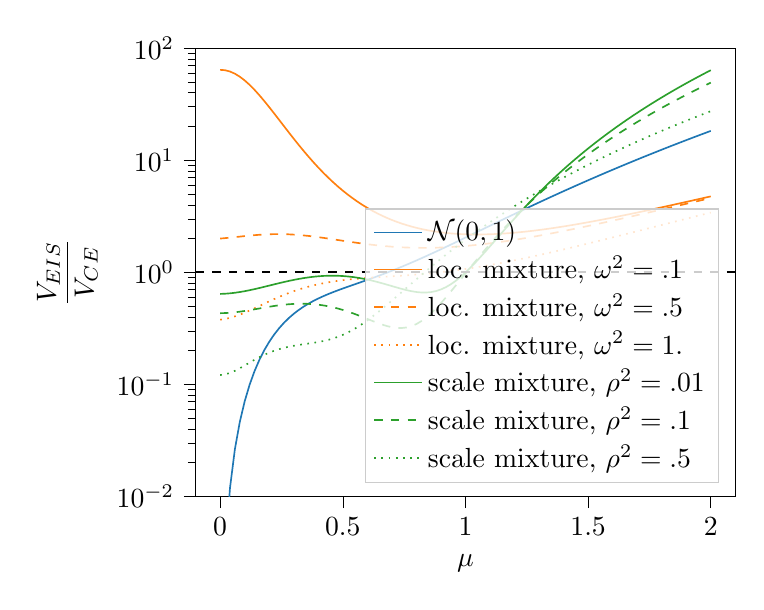
\begin{tikzpicture}

\definecolor{darkgray176}{RGB}{176,176,176}
\definecolor{darkorange25512714}{RGB}{255,127,14}
\definecolor{forestgreen4416044}{RGB}{44,160,44}
\definecolor{lightgray204}{RGB}{204,204,204}
\definecolor{steelblue31119180}{RGB}{31,119,180}

\begin{axis}[
legend cell align={left},
legend style={
  fill opacity=0.8,
  draw opacity=1,
  text opacity=1,
  at={(0.97,0.03)},
  anchor=south east,
  draw=lightgray204
},
log basis y={10},
tick align=outside,
tick pos=left,
x grid style={darkgray176},
xlabel={\(\displaystyle \mu\)},
xmin=-0.1, xmax=2.1,
xtick style={color=black},
y grid style={darkgray176},
ylabel={\(\displaystyle \frac{V_{\text{EIS}}}{V_{\text{CE}}}\)},
ymin=0.01, ymax=100,
ymode=log,
ytick style={color=black}
]
\addplot [semithick, steelblue31119180]
table {%
0 0
0.0199999995529652 0.00299281300976872
0.0399999991059303 0.0118856830522418
0.0599999986588955 0.0264268033206463
0.0799999982118607 0.0462124161422253
0.0999999940395355 0.0707092434167862
0.119999997317791 0.0992832705378532
0.140000000596046 0.131232619285583
0.159999996423721 0.165821358561516
0.179999992251396 0.202313810586929
0.199999988079071 0.240004301071167
0.219999998807907 0.278243839740753
0.239999994635582 0.31645929813385
0.259999990463257 0.35416966676712
0.280000001192093 0.390992254018784
0.299999982118607 0.426646500825882
0.319999992847443 0.46095085144043
0.340000003576279 0.493818193674088
0.359999984502792 0.525244355201721
0.379999995231628 0.555299520492554
0.399999976158142 0.584115505218506
0.419999986886978 0.611874043941498
0.439999997615814 0.638795375823975
0.459999978542328 0.665127098560333
0.479999989271164 0.691136360168457
0.5 0.717100322246552
0.519999980926514 0.743300557136536
0.539999961853027 0.770016372203827
0.560000002384186 0.797523856163025
0.579999983310699 0.826088905334473
0.599999964237213 0.855968296527863
0.620000004768372 0.887409210205078
0.639999985694885 0.920644283294678
0.659999966621399 0.955896973609924
0.680000007152557 0.993378877639771
0.699999988079071 1.03329133987427
0.719999969005585 1.0758261680603
0.740000009536743 1.1211678981781
0.759999990463257 1.16949236392975
0.779999971389771 1.22096979618073
0.799999952316284 1.27576732635498
0.819999992847443 1.33404433727264
0.839999973773956 1.39596247673035
0.85999995470047 1.46167659759521
0.879999995231628 1.53134441375732
0.899999976158142 1.6051197052002
0.919999957084656 1.68316090106964
0.939999997615814 1.76562368869781
0.959999978542328 1.85266888141632
0.979999959468842 1.94445705413818
1 2.04115223884583
1.01999998092651 2.14292287826538
1.03999996185303 2.24993705749512
1.05999994277954 2.36237406730652
1.07999992370605 2.48040914535522
1.10000002384186 2.60422539710999
1.12000000476837 2.73401188850403
1.13999998569489 2.86996269226074
1.1599999666214 3.01227259635925
1.17999994754791 3.16114592552185
1.19999992847443 3.31679320335388
1.22000002861023 3.47942614555359
1.24000000953674 3.64926242828369
1.25999999046326 3.82653069496155
1.27999997138977 4.01145696640015
1.29999995231628 4.20428419113159
1.3199999332428 4.40524911880493
1.33999991416931 4.61460781097412
1.36000001430511 4.83261156082153
1.37999999523163 5.0595235824585
1.39999997615814 5.29561042785645
1.41999995708466 5.54114484786987
1.43999993801117 5.79641771316528
1.45999991893768 6.06170701980591
1.48000001907349 6.33731842041016
1.5 6.62354278564453
1.51999998092651 6.92069721221924
1.53999996185303 7.2290940284729
1.55999994277954 7.54905796051025
1.57999992370605 7.88092231750488
1.59999990463257 8.22502326965332
1.62000000476837 8.58170700073242
1.63999998569489 8.95132637023926
1.6599999666214 9.33424663543701
1.67999994754791 9.73083209991455
1.69999992847443 10.1414632797241
1.71999990940094 10.5665254592896
1.74000000953674 11.0064125061035
1.75999999046326 11.461519241333
1.77999997138977 11.9322690963745
1.79999995231628 12.4190721511841
1.8199999332428 12.9223594665527
1.83999991416931 13.4425640106201
1.86000001430511 13.9801349639893
1.87999999523163 14.5355319976807
1.89999997615814 15.109203338623
1.91999995708466 15.7016410827637
1.93999993801117 16.3133029937744
1.95999991893768 16.944709777832
1.9799998998642 17.596342086792
2 18.268726348877
};
\addlegendentry{$\mathcal N (0,1)$}
\addplot [semithick, darkorange25512714]
table {%
0 64.064826965332
0.0199999995529652 63.5564765930176
0.0399999991059303 61.8869285583496
0.0599999986588955 59.1853523254395
0.0799999982118607 55.6484870910645
0.0999999940395355 51.5253372192383
0.119999997317791 47.0613288879395
0.140000000596046 42.4868774414062
0.159999996423721 37.9917297363281
0.179999992251396 33.7195587158203
0.199999988079071 29.7637310028076
0.219999998807907 26.1763401031494
0.239999994635582 22.974588394165
0.259999990463257 20.1525440216064
0.280000001192093 17.6916198730469
0.299999982118607 15.5568208694458
0.319999992847443 13.7170066833496
0.340000003576279 12.134391784668
0.359999984502792 10.7763261795044
0.379999995231628 9.61130809783936
0.399999976158142 8.61177158355713
0.419999986886978 7.75361347198486
0.439999997615814 7.01570272445679
0.459999978542328 6.37912464141846
0.479999989271164 5.82968711853027
0.5 5.35449600219727
0.519999980926514 4.94199657440186
0.539999961853027 4.58309888839722
0.560000002384186 4.27036666870117
0.579999983310699 3.99697470664978
0.599999964237213 3.75787019729614
0.620000004768372 3.54797673225403
0.639999985694885 3.36348152160645
0.659999966621399 3.20135378837585
0.680000007152557 3.05821967124939
0.699999988079071 2.9323935508728
0.719999969005585 2.82139372825623
0.740000009536743 2.72358298301697
0.759999990463257 2.63746047019958
0.779999971389771 2.56183743476868
0.799999952316284 2.49527978897095
0.819999992847443 2.43728399276733
0.839999973773956 2.38683366775513
0.85999995470047 2.34301543235779
0.879999995231628 2.30551099777222
0.899999976158142 2.27377128601074
0.919999957084656 2.24694991111755
0.939999997615814 2.22512435913086
0.959999978542328 2.20764780044556
0.979999959468842 2.19421529769897
1 2.18456244468689
1.01999998092651 2.17864918708801
1.03999996185303 2.17585444450378
1.05999994277954 2.17647910118103
1.07999992370605 2.18004703521729
1.10000002384186 2.18641591072083
1.12000000476837 2.19540619850159
1.13999998569489 2.20709609985352
1.1599999666214 2.22135066986084
1.17999994754791 2.23808813095093
1.19999992847443 2.25703525543213
1.22000002861023 2.27835249900818
1.24000000953674 2.30202317237854
1.25999999046326 2.32757210731506
1.27999997138977 2.35555171966553
1.29999995231628 2.38543725013733
1.3199999332428 2.41768479347229
1.33999991416931 2.45174646377563
1.36000001430511 2.48791718482971
1.37999999523163 2.52616000175476
1.39999997615814 2.56625628471375
1.41999995708466 2.60849761962891
1.43999993801117 2.6527304649353
1.45999991893768 2.69915628433228
1.48000001907349 2.74737453460693
1.5 2.79764103889465
1.51999998092651 2.84996914863586
1.53999996185303 2.90410327911377
1.55999994277954 2.96054601669312
1.57999992370605 3.01908349990845
1.59999990463257 3.07936835289001
1.62000000476837 3.14185380935669
1.63999998569489 3.20663237571716
1.6599999666214 3.27349972724915
1.67999994754791 3.3422269821167
1.69999992847443 3.41333818435669
1.71999990940094 3.4867217540741
1.74000000953674 3.56236910820007
1.75999999046326 3.64020657539368
1.77999997138977 3.72048020362854
1.79999995231628 3.80220317840576
1.8199999332428 3.88699460029602
1.83999991416931 3.97393751144409
1.86000001430511 4.06380605697632
1.87999999523163 4.15581321716309
1.89999997615814 4.24964284896851
1.91999995708466 4.34675121307373
1.93999993801117 4.44652795791626
1.95999991893768 4.54832172393799
1.9799998998642 4.65282487869263
2 4.76013040542603
};
\addlegendentry{loc. mixture, $\omega^2 = .1$}
\addplot [semithick, darkorange25512714, dashed]
table {%
0 2.00069522857666
0.0199999995529652 2.01893544197083
0.0399999991059303 2.03916788101196
0.0599999986588955 2.06059384346008
0.0799999982118607 2.08271288871765
0.0999999940395355 2.104811668396
0.119999997317791 2.12611389160156
0.140000000596046 2.14572048187256
0.159999996423721 2.16260409355164
0.179999992251396 2.17632699012756
0.199999988079071 2.18627309799194
0.219999998807907 2.19204640388489
0.239999994635582 2.19331979751587
0.259999990463257 2.19000911712646
0.280000001192093 2.18212580680847
0.299999982118607 2.17002725601196
0.319999992847443 2.15391874313354
0.340000003576279 2.13435339927673
0.359999984502792 2.11190557479858
0.379999995231628 2.08684968948364
0.399999976158142 2.05977344512939
0.419999986886978 2.03130769729614
0.439999997615814 2.00194215774536
0.459999978542328 1.9720733165741
0.479999989271164 1.94231700897217
0.5 1.91301023960114
0.519999980926514 1.88432276248932
0.539999961853027 1.8565262556076
0.560000002384186 1.83018958568573
0.579999983310699 1.80532610416412
0.599999964237213 1.78206503391266
0.620000004768372 1.76049137115479
0.639999985694885 1.74076700210571
0.659999966621399 1.72314190864563
0.680000007152557 1.70743608474731
0.699999988079071 1.69368612766266
0.719999969005585 1.68187594413757
0.740000009536743 1.67216825485229
0.759999990463257 1.66455709934235
0.779999971389771 1.65888130664825
0.799999952316284 1.65507483482361
0.819999992847443 1.65333020687103
0.839999973773956 1.65329813957214
0.85999995470047 1.65522015094757
0.879999995231628 1.65903806686401
0.899999976158142 1.66466951370239
0.919999957084656 1.67203342914581
0.939999997615814 1.68107354640961
0.959999978542328 1.69188868999481
0.979999959468842 1.70455515384674
1 1.71860444545746
1.01999998092651 1.7344559431076
1.03999996185303 1.75194537639618
1.05999994277954 1.77100145816803
1.07999992370605 1.79161584377289
1.10000002384186 1.81383836269379
1.12000000476837 1.83763337135315
1.13999998569489 1.86311709880829
1.1599999666214 1.89009070396423
1.17999994754791 1.91854846477509
1.19999992847443 1.94862055778503
1.22000002861023 1.98023450374603
1.24000000953674 2.01352310180664
1.25999999046326 2.04807043075562
1.27999997138977 2.08449840545654
1.29999995231628 2.1223464012146
1.3199999332428 2.16183733940125
1.33999991416931 2.20312261581421
1.36000001430511 2.24573850631714
1.37999999523163 2.28995490074158
1.39999997615814 2.33602571487427
1.41999995708466 2.38379645347595
1.43999993801117 2.43310904502869
1.45999991893768 2.48427653312683
1.48000001907349 2.53690695762634
1.5 2.59157562255859
1.51999998092651 2.64779663085938
1.53999996185303 2.70588898658752
1.55999994277954 2.76579260826111
1.57999992370605 2.82734560966492
1.59999990463257 2.89090061187744
1.62000000476837 2.95633316040039
1.63999998569489 3.02378416061401
1.6599999666214 3.09329605102539
1.67999994754791 3.16447877883911
1.69999992847443 3.23782467842102
1.71999990940094 3.31328535079956
1.74000000953674 3.39060592651367
1.75999999046326 3.47004723548889
1.77999997138977 3.55179619789124
1.79999995231628 3.6357638835907
1.8199999332428 3.72163438796997
1.83999991416931 3.80955243110657
1.86000001430511 3.8999650478363
1.87999999523163 3.99296545982361
1.89999997615814 4.08828449249268
1.91999995708466 4.18591403961182
1.93999993801117 4.28575134277344
1.95999991893768 4.38834714889526
1.9799998998642 4.49317741394043
2 4.60064125061035
};
\addlegendentry{loc. mixture, $\omega^2 = .5$}
\addplot [semithick, darkorange25512714, dotted]
table {%
0 0.3780198097229
0.0199999995529652 0.383591026067734
0.0399999991059303 0.392346382141113
0.0599999986588955 0.40420338511467
0.0799999982118607 0.418912380933762
0.0999999940395355 0.436240971088409
0.119999997317791 0.455965578556061
0.140000000596046 0.477641761302948
0.159999996423721 0.501008272171021
0.179999992251396 0.525627076625824
0.199999988079071 0.551053047180176
0.219999998807907 0.576954126358032
0.239999994635582 0.603023767471313
0.259999990463257 0.628755748271942
0.280000001192093 0.654045879840851
0.299999982118607 0.678528308868408
0.319999992847443 0.701861083507538
0.340000003576279 0.724102556705475
0.359999984502792 0.744918167591095
0.379999995231628 0.764307200908661
0.399999976158142 0.782261312007904
0.419999986886978 0.798586308956146
0.439999997615814 0.813658356666565
0.459999978542328 0.827271640300751
0.479999989271164 0.839538156986237
0.5 0.850645899772644
0.519999980926514 0.860495567321777
0.539999961853027 0.86939525604248
0.560000002384186 0.877569258213043
0.579999983310699 0.884868383407593
0.599999964237213 0.891722738742828
0.620000004768372 0.898136675357819
0.639999985694885 0.904202580451965
0.659999966621399 0.91007274389267
0.680000007152557 0.915912866592407
0.699999988079071 0.921836674213409
0.719999969005585 0.927826166152954
0.740000009536743 0.934146344661713
0.759999990463257 0.940782427787781
0.779999971389771 0.947908997535706
0.799999952316284 0.955457746982574
0.819999992847443 0.963574945926666
0.839999973773956 0.972351908683777
0.85999995470047 0.981722056865692
0.879999995231628 0.991853892803192
0.899999976158142 1.00293302536011
0.919999957084656 1.01468622684479
0.939999997615814 1.02721726894379
0.959999978542328 1.04079449176788
0.979999959468842 1.0552282333374
1 1.07043588161469
1.01999998092651 1.0867714881897
1.03999996185303 1.10398888587952
1.05999994277954 1.12225472927094
1.07999992370605 1.14145112037659
1.10000002384186 1.16178297996521
1.12000000476837 1.18317472934723
1.13999998569489 1.20562529563904
1.1599999666214 1.22905290126801
1.17999994754791 1.25363302230835
1.19999992847443 1.2791930437088
1.22000002861023 1.30598258972168
1.24000000953674 1.33391487598419
1.25999999046326 1.36300957202911
1.27999997138977 1.39324820041656
1.29999995231628 1.42462730407715
1.3199999332428 1.45722818374634
1.33999991416931 1.49101066589355
1.36000001430511 1.52612435817719
1.37999999523163 1.56234955787659
1.39999997615814 1.59977674484253
1.41999995708466 1.6385657787323
1.43999993801117 1.67867243289948
1.45999991893768 1.72011995315552
1.48000001907349 1.76275265216827
1.5 1.80691862106323
1.51999998092651 1.85232508182526
1.53999996185303 1.89904987812042
1.55999994277954 1.94736993312836
1.57999992370605 1.99692583084106
1.59999990463257 2.04835987091064
1.62000000476837 2.10073494911194
1.63999998569489 2.15497756004333
1.6599999666214 2.21064519882202
1.67999994754791 2.26769685745239
1.69999992847443 2.32651782035828
1.71999990940094 2.38669061660767
1.74000000953674 2.44890451431274
1.75999999046326 2.51238441467285
1.77999997138977 2.57789444923401
1.79999995231628 2.64457964897156
1.8199999332428 2.71349453926086
1.83999991416931 2.78379058837891
1.86000001430511 2.85617685317993
1.87999999523163 2.93024301528931
1.89999997615814 3.006023645401
1.91999995708466 3.08377742767334
1.93999993801117 3.16390132904053
1.95999991893768 3.24548172950745
1.9799998998642 3.32905507087708
2 3.41476202011108
};
\addlegendentry{loc. mixture, $\omega^2 = 1.$}
\addplot [semithick, forestgreen4416044]
table {%
0 0.641549170017242
0.0199999995529652 0.64431893825531
0.0399999991059303 0.649595081806183
0.0599999986588955 0.657183468341827
0.0799999982118607 0.667025923728943
0.0999999940395355 0.678922235965729
0.119999997317791 0.69266951084137
0.140000000596046 0.708047330379486
0.159999996423721 0.72487860918045
0.179999992251396 0.742746412754059
0.199999988079071 0.761478185653687
0.219999998807907 0.780706763267517
0.239999994635582 0.800100564956665
0.259999990463257 0.819344460964203
0.280000001192093 0.838056325912476
0.299999982118607 0.855963170528412
0.319999992847443 0.872696399688721
0.340000003576279 0.887921333312988
0.359999984502792 0.90135669708252
0.379999995231628 0.912797629833221
0.399999976158142 0.921839535236359
0.419999986886978 0.928400635719299
0.439999997615814 0.932246029376984
0.459999978542328 0.933306455612183
0.479999989271164 0.931405127048492
0.5 0.926657855510712
0.519999980926514 0.918972373008728
0.539999961853027 0.908493518829346
0.560000002384186 0.895359694957733
0.579999983310699 0.879699409008026
0.599999964237213 0.861952662467957
0.620000004768372 0.842281997203827
0.639999985694885 0.821190237998962
0.659999966621399 0.799105584621429
0.680000007152557 0.776510059833527
0.699999988079071 0.753969848155975
0.719999969005585 0.732140600681305
0.740000009536743 0.711811482906342
0.759999990463257 0.693664908409119
0.779999971389771 0.678595244884491
0.799999952316284 0.667292058467865
0.819999992847443 0.660893797874451
0.839999973773956 0.660263419151306
0.85999995470047 0.666379451751709
0.879999995231628 0.680451810359955
0.899999976158142 0.703445613384247
0.919999957084656 0.73673552274704
0.939999997615814 0.781327962875366
0.959999978542328 0.838589429855347
0.979999959468842 0.909819364547729
1 0.996338188648224
1.01999998092651 1.09936475753784
1.03999996185303 1.22058129310608
1.05999994277954 1.36126148700714
1.07999992370605 1.52287292480469
1.10000002384186 1.707066655159
1.12000000476837 1.91545069217682
1.13999998569489 2.14914798736572
1.1599999666214 2.41020560264587
1.17999994754791 2.70034289360046
1.19999992847443 3.02098512649536
1.22000002861023 3.37364840507507
1.24000000953674 3.760498046875
1.25999999046326 4.18283939361572
1.27999997138977 4.64322566986084
1.29999995231628 5.14264059066772
1.3199999332428 5.68347024917603
1.33999991416931 6.26725339889526
1.36000001430511 6.89635229110718
1.37999999523163 7.57224369049072
1.39999997615814 8.29694747924805
1.41999995708466 9.07260704040527
1.43999993801117 9.90093803405762
1.45999991893768 10.7841854095459
1.48000001907349 11.725682258606
1.5 12.7248392105103
1.51999998092651 13.7860450744629
1.53999996185303 14.9098329544067
1.55999994277954 16.1001052856445
1.57999992370605 17.3562240600586
1.59999990463257 18.6850242614746
1.62000000476837 20.0837936401367
1.63999998569489 21.5580883026123
1.6599999666214 23.1086921691895
1.67999994754791 24.7392253875732
1.69999992847443 26.4509201049805
1.71999990940094 28.2454490661621
1.74000000953674 30.1250629425049
1.75999999046326 32.097225189209
1.77999997138977 34.160285949707
1.79999995231628 36.3134269714355
1.8199999332428 38.5633316040039
1.83999991416931 40.9151802062988
1.86000001430511 43.3655815124512
1.87999999523163 45.9222755432129
1.89999997615814 48.5809288024902
1.91999995708466 51.3525352478027
1.93999993801117 54.2337951660156
1.95999991893768 57.2334403991699
1.9799998998642 60.3448219299316
2 63.5767211914062
};
\addlegendentry{scale mixture, $\rho^2 = .01$}
\addplot [semithick, forestgreen4416044, dashed]
table {%
0 0.431960076093674
0.0199999995529652 0.433056831359863
0.0399999991059303 0.435767710208893
0.0599999986588955 0.439941495656967
0.0799999982118607 0.44542595744133
0.0999999940395355 0.452016234397888
0.119999997317791 0.459490418434143
0.140000000596046 0.467592298984528
0.159999996423721 0.476054310798645
0.179999992251396 0.484580397605896
0.199999988079071 0.492943942546844
0.219999998807907 0.500804126262665
0.239999994635582 0.507913053035736
0.259999990463257 0.514079451560974
0.280000001192093 0.519017457962036
0.299999982118607 0.522522687911987
0.319999992847443 0.524489223957062
0.340000003576279 0.524686455726624
0.359999984502792 0.523108839988708
0.379999995231628 0.519682228565216
0.399999976158142 0.514378011226654
0.419999986886978 0.507175981998444
0.439999997615814 0.49819153547287
0.459999978542328 0.487561643123627
0.479999989271164 0.475366055965424
0.5 0.46187162399292
0.519999980926514 0.447269201278687
0.539999961853027 0.431858837604523
0.560000002384186 0.415910810232162
0.579999983310699 0.399799138307571
0.599999964237213 0.383918792009354
0.620000004768372 0.368691802024841
0.639999985694885 0.354550391435623
0.659999966621399 0.342012405395508
0.680000007152557 0.331595987081528
0.699999988079071 0.323786348104477
0.719999969005585 0.319222748279572
0.740000009536743 0.318477779626846
0.759999990463257 0.322177350521088
0.779999971389771 0.331035614013672
0.799999952316284 0.345633983612061
0.819999992847443 0.366783529520035
0.839999973773956 0.395111232995987
0.85999995470047 0.431392908096313
0.879999995231628 0.476510286331177
0.899999976158142 0.531041920185089
0.919999957084656 0.595907509326935
0.939999997615814 0.672023236751556
0.959999978542328 0.760107338428497
0.979999959468842 0.86113303899765
1 0.975934863090515
1.01999998092651 1.10541725158691
1.03999996185303 1.25050210952759
1.05999994277954 1.41215014457703
1.07999992370605 1.59141767024994
1.10000002384186 1.78918254375458
1.12000000476837 2.00641775131226
1.13999998569489 2.24426865577698
1.1599999666214 2.50348520278931
1.17999994754791 2.78554940223694
1.19999992847443 3.09129929542542
1.22000002861023 3.42165207862854
1.24000000953674 3.77817273139954
1.25999999046326 4.16154623031616
1.27999997138977 4.57310009002686
1.29999995231628 5.01390361785889
1.3199999332428 5.48514127731323
1.33999991416931 5.98850870132446
1.36000001430511 6.52421522140503
1.37999999523163 7.09415864944458
1.39999997615814 7.70020008087158
1.41999995708466 8.34212303161621
1.43999993801117 9.02214241027832
1.45999991893768 9.74127292633057
1.48000001907349 10.5009927749634
1.5 11.3029270172119
1.51999998092651 12.1473913192749
1.53999996185303 13.0371160507202
1.55999994277954 13.9729070663452
1.57999992370605 14.9544773101807
1.59999990463257 15.98681640625
1.62000000476837 17.0685005187988
1.63999998569489 18.2016181945801
1.6599999666214 19.3886241912842
1.67999994754791 20.6310119628906
1.69999992847443 21.9286193847656
1.71999990940094 23.2820262908936
1.74000000953674 24.6971664428711
1.75999999046326 26.1724376678467
1.77999997138977 27.7106800079346
1.79999995231628 29.3114318847656
1.8199999332428 30.9794292449951
1.83999991416931 32.7136878967285
1.86000001430511 34.5172996520996
1.87999999523163 36.3912544250488
1.89999997615814 38.3366241455078
1.91999995708466 40.3568916320801
1.93999993801117 42.4531707763672
1.95999991893768 44.6266937255859
1.9799998998642 46.8779067993164
2 49.2078704833984
};
\addlegendentry{scale mixture, $\rho^2 = .1$}
\addplot [semithick, forestgreen4416044, dotted]
table {%
0 0.121202975511551
0.0199999995529652 0.122827485203743
0.0399999991059303 0.126581713557243
0.0599999986588955 0.132203876972198
0.0799999982118607 0.139320194721222
0.0999999940395355 0.147537857294083
0.119999997317791 0.156492650508881
0.140000000596046 0.165712624788284
0.159999996423721 0.174919486045837
0.179999992251396 0.18379034101963
0.199999988079071 0.192084923386574
0.219999998807907 0.199579149484634
0.239999994635582 0.206233218312263
0.259999990463257 0.212016507983208
0.280000001192093 0.216982245445251
0.299999982118607 0.221204429864883
0.319999992847443 0.22487773001194
0.340000003576279 0.228213861584663
0.359999984502792 0.231481283903122
0.379999995231628 0.234899446368217
0.399999976158142 0.2388616502285
0.419999986886978 0.243608683347702
0.439999997615814 0.249434918165207
0.459999978542328 0.256711393594742
0.479999989271164 0.265735507011414
0.5 0.276754647493362
0.519999980926514 0.290141433477402
0.539999961853027 0.306143820285797
0.560000002384186 0.324998885393143
0.579999983310699 0.347046375274658
0.599999964237213 0.37250155210495
0.620000004768372 0.401553124189377
0.639999985694885 0.434563517570496
0.659999966621399 0.47167244553566
0.680000007152557 0.513170957565308
0.699999988079071 0.559247255325317
0.719999969005585 0.610128819942474
0.740000009536743 0.665990650653839
0.759999990463257 0.727211236953735
0.779999971389771 0.793849647045135
0.799999952316284 0.86616313457489
0.819999992847443 0.944479048252106
0.839999973773956 1.02896189689636
0.85999995470047 1.11980056762695
0.879999995231628 1.21729755401611
0.899999976158142 1.32162249088287
0.919999957084656 1.43319511413574
0.939999997615814 1.55205357074738
0.959999978542328 1.67853903770447
0.979999959468842 1.81309962272644
1 1.95563971996307
1.01999998092651 2.10671281814575
1.03999996185303 2.26648712158203
1.05999994277954 2.43537926673889
1.07999992370605 2.61347460746765
1.10000002384186 2.80138826370239
1.12000000476837 2.99910187721252
1.13999998569489 3.20709419250488
1.1599999666214 3.42573642730713
1.17999994754791 3.65518379211426
1.19999992847443 3.89602303504944
1.22000002861023 4.14815378189087
1.24000000953674 4.41241598129272
1.25999999046326 4.6890082359314
1.27999997138977 4.97817993164062
1.29999995231628 5.28051900863647
1.3199999332428 5.59601020812988
1.33999991416931 5.92562246322632
1.36000001430511 6.26900959014893
1.37999999523163 6.62697219848633
1.39999997615814 7.00068664550781
1.41999995708466 7.3888988494873
1.43999993801117 7.79298543930054
1.45999991893768 8.21372413635254
1.48000001907349 8.65087413787842
1.5 9.10478591918945
1.51999998092651 9.57632350921631
1.53999996185303 10.0661001205444
1.55999994277954 10.5744380950928
1.57999992370605 11.1009254455566
1.59999990463257 11.6468868255615
1.62000000476837 12.2130117416382
1.63999998569489 12.7992753982544
1.6599999666214 13.4059896469116
1.67999994754791 14.0341806411743
1.69999992847443 14.6842613220215
1.71999990940094 15.3561315536499
1.74000000953674 16.0509414672852
1.75999999046326 16.7691287994385
1.77999997138977 17.5110683441162
1.79999995231628 18.2770843505859
1.8199999332428 19.0684509277344
1.83999991416931 19.8845062255859
1.86000001430511 20.7268753051758
1.87999999523163 21.5960102081299
1.89999997615814 22.4912719726562
1.91999995708466 23.4140129089355
1.93999993801117 24.3672466278076
1.95999991893768 25.3471813201904
1.9799998998642 26.3551006317139
2 27.3943290710449
};
\addlegendentry{scale mixture, $\rho^2 = .5$}
\addplot [semithick, black, dashed, forget plot]
table {%
-0.1 1
2.1 1
};
\end{axis}

\end{tikzpicture}
%
            }
        \end{subfigure}
        \label{fig:normal_are}
        \caption{Asymptotic relative efficiency $\frac{V_{\eis}}{V_{\ce}}$ for the normal distribution from \Cref{ex:univ-gaussian-s2-fixed} (left hand side) and \Cref{ex:univ-gaussian-mu-fixed} (right hand side). Here $\P = \mathcal N(0, 1)$ is the standard normal distribution and $\G = \mathcal N(\mu, \sigma^{2})$, where either $\sigma^{2}$ is fixed (left) and $\mu$ determined by the \gls{cem} / \gls{eis}, or the other way around (right). Notice the log scale of the $y$-axis. As $\mu$ or $\sigma^{2}$ get close to their true values, \gls{eis} outperforms the \gls{cem} in terms of asymptotic variance, see {\color{red} todo:  reference to example where EIS is exact.}. As}
    \end{figure}
    

    %\begin{table}
    %    \centering
    %    \begin{tabular}{ccc}
    %        \toprule
    %        & $\sigma^{2}$ fixed, $\tau^{2} \to \infty$ & $\tau^{2}$ fixed, $\sigma^{2} \to \infty$\\
    %        \midrule
    %        $V_{\ce} / V_{\eis}$ & $\frac{2}{5} \sigma^{2}$ & 0 \\
    %        \bottomrule
    %    \end{tabular}
    %    \caption{Relative asymptotic efficiencies of the \gls{cem} and \gls{eis} for \Cref{ex:univ-gaussian-s2-fixed} and \Cref{ex:univ-gaussian-mu-fixed}.}
    %    \label{tab:comparison-asymptotics}
    %\end{table}
    
    \paragraph{Gaussian location mixture}
    Consider now the case where $\P = \frac{1}{2} \mathcal N(-1, \omega^{2}) + \frac{1}{2}\mathcal N(1, \omega^{2})$ is a Gaussian location mixture. The second moment is $\tau^{2} = 1 + \omega^{2} = -\frac{1}{2\pce}$. Unfortunately, there is no closed-form expression for many of the terms required for the analysis \gls{eis}. Instead, we resort to a simulation study to determine the asymptotic variances and relative efficiencies.

    \todo{numerical example: GMM}
    \todo{interpretation: if variance set too low, CE better. if variance too big EIS better}
    
\end{example}

\begin{example}[univariate Gaussian, $\mu$ fixed]
    \label{ex:univ-gaussian-mu-fixed}
    Consider the same setup as in \Cref{ex:univ-gaussian-s2-fixed}, i.e. $\P$ is symmetric around $0$ with second moment $\tau^{2}$, but let $\G_{\psi} = \mathcal N(\mu, -\frac{1}{2\psi})$ be the single parameter natural exponential family of Gaussians with fixed mean $\mu$ and variance $\sigma^{2} = -\frac{1}{2 \psi}$. 
    
    Then
    $$
    \log g_{\psi}(x) = \psi T(x) + \frac{1}{2}\log \left( - 2 \psi \right) - \frac{1}{2} \log 2\pi
    $$
    for $T(x) = (x - \mu)^{2}$. Thus $\P T = \tau^{2} + \mu^{2}$ and $\cov_{\P} T = \nu - \tau^{4} + 4\tau^{2}\mu^{2}$ where $\nu = \P \operatorname{id}^{4}$ and $\tau^{2} = \P \id^{2}$. 
    %\paragraph{\Acrlong{cem}}

    By matching moments, we obtain $\pce = -\frac{1}{2(\tau^{2} + \mu^{2})}$ and $I(\pce) = \frac{1}{2\pce^{2}} = 2(\tau^{2} + \mu^{2})^{2}$. In total 
    \begin{align}
        V_{\ce} &= \frac{1}{4 (\tau^{2} + \mu^{2})^{4}} \left( \nu - \tau^{4} + 4\tau^{2}\mu^{2} \right)
    \end{align}

    %\paragraph{\Acrlong{eis}}
    For \gls{eis},
    \begin{align*}
    \peis &= \left( \cov_{\P} T \right)^{-1} \cov_{\P} \left( T, \log p \right) \\
        &= \left( \nu - \tau^{4} + 4\tau^{2}\mu^{2} \right)^{-1} \underbrace{\int p(x)((x-\mu)^{2}-\tau^{2} - \mu^{2})(\log p(x) - \P\log p(x)) \d x}_{=\gamma}.
    \end{align*}
    
    Then 
    \begin{align*}
        V_{\eis} = \left( \nu - \tau^{4} + 4 \tau^{2}\mu^{2}\right)^{-2} \P \left( (\id - \mu)^{4} \left( \log p - \peis (\id - \mu)^{2} - \P \log p + \psi (\tau^{2} + \mu^{2}) \right)^{2} \right).
    \end{align*}

    \paragraph{Normal distribution}
    Consider now the normal distribution $\P = \mathcal N (0, \tau^{2})$ where $\nu = 3 \tau^{4}$ and $\gamma = -\tau^{2}$, so 
    \begin{align*}
        \peis &= \frac{-\tau^{2}}{2\tau^{2} \left( \tau^{2} + 2\mu^{2} \right)} = \frac{-1}{2(\tau^{2} + 2\mu^{2})}.
    \end{align*}
    Thus the \gls{eis} proposal uses variance $\sigma^{2}_{\eis} = \tau^{2} + 2\mu^{2}$, which is bigger than the variance of $\sigma^{2}_{\ce} = \tau^{2} + \mu^{2}$ optimal for the \gls{cem}.

    In this case the asymptotic variances are
    \begin{align*}
    %\label{eq:asymptotic-vars}
        V_{\ce} &= \frac{\tau^{2}(\tau^{2} + 2\mu^{2})}{2 \left( \tau^{2} + \mu^{2} \right)^{4}}\\
        \intertext{and}
        V_{\eis} &= \frac{\mu^{2} \left(2 \mu^{6} + 45 \mu^{4} \tau^{2} + 15 \tau^{6}\right)}{4 \tau^{4} \left(2 \mu^{2} + \tau^{2}\right)^{4}},
    \end{align*}
    see the accompanying source code for their calculation in sympy \todo{ref it}.
\end{example}


% rationale
In applications, e.g. the model studied in \Cref{cha:analysis_of_selected_models}, we are interested in the performance of the importance sampling proposals generated by the \gls{la}, \gls{cem} and \gls{eis} under more complex circumstances than those discussed in \Cref{ex:univ-gaussian-mu-fixed,ex:univ-gaussian-s2-fixed}. In particular, the dimension of $\psi$ is high ($\mathcal O(n \cdot m)$ or even $\mathcal O(n \cdot m^{2})$) and proposals may not come from a natural exponential family, so analysis based on \Cref{thm:ce-clt,thm:clt-eis} is not possible. Instead, we resort to simulation studies to gain insights into the circumstances when one should prefer one method over the other.
As a leading example, we will use the following vector-autoregressive state space model with negative binomial observations. A similar, though more involved, model is studied in \Cref{sec:regional_growth_factor_model} with real data.

\begin{example}[Negative Binomial $\operatorname{VAR}(1)$ \gls{ssm}]
    \label{ex:negbinom-ar1}
    % setup 
    In this example, we consider a \gls{ssm} where states $X_{t}$ follow a stationary Gaussian $\operatorname{VAR}(1)$ process, initialized in its stationary distribution $\mathcal N(0,\Sigma)$. For simplicity let the transition matrices be given by a multiple of the identity, i.e. $A_{t} = \alpha I_{m}$ for all $t$ where $\alpha \in (-1, 1)$ \todo{add I to symbols}. 
    In total, the model is given by
    \begin{align*}
    X_{0} &\sim \mathcal N(0,\Sigma) \\
    X_{t} &= \alpha X_{t - 1} + \varepsilon_{t}\\
    \varepsilon_t &\iid \mathcal N(0, (1 - \alpha^{2})\Sigma), t = 1, \dots, n
    \end{align*}
    where the $\varepsilon_{1}, \dots, n$ and $X_{0}$ are jointly independent. The observations follow a conditional negative binomial distribution 
    $$
    Y^{i}_{t} | X_{t} \sim \nbinom \left( \exp{X^{i}_{t}}, r \right), i = 1, \dots, p
    $$
    where the parametrization is the one by mean and overdispersion parameter $r > 0$ \todo{ref it} and individual observations are conditionally independent given the current state.
\end{example}

%% simulation study on MSE/Bias/Variance

Our first simulation study concerns the non-asymptotic behavior of the \gls{cem} and \gls{eis} estimators, i.e. finite sample analogs of \Cref{thm:ce-clt,thm:clt-eis}. To this end,
we let $m = 1$ in \Cref{ex:negbinom-ar1} and fix $n$ to \todo{...}. 
We then simulate once from the marginal distribution of $Y$ and perform the \gls{la} to a prespecified precision $\epsilon$ and maximum number of iterations $n_{\text{iter}}$, obtaining a proposal distribution $\G_{\la}$. Using a large number of samples $N_{\text{true}}$ from this proposal we find the optimal $\G_{\ce}$ and $\G_{\eis}$ using the same desired precision and number of iterations as for the \gls{la}. For the remainder of this section, we ignore sampling variation in these proposals and treat them as exact. 

%% posterior marginal means and variances
To determine the non-asymptotic sampling behavior we now perform the above procedure again, using only $N \ll N_{\text{true}}$ many samples for both procedures, obtaining proposals $\hat\P^{N}_{\ce}$ and $\hat \P^{N}_{\eis}$. As the full proposals are Gaussian distributions on $\R^{(n+1)\times m}$, either given as the posterior of a \gls{glssm} (\gls{la}, \gls{eis}) or by mean and Cholesky root of the precision matrix(\gls{cem}). 
This procedure is repeated $M$ times for every sample size $N$ considered, with different initial random seeds, obtaining $\hat\P^{N,i}_{\ce}$ and $\hat \P^{N,i}_{\eis}$ for $i = 1, \dots, M$.

To assess the speed of convergence of the \gls{cem} and \gls{eis} we then estimate the mean squared error of means and variances of the $(n+1) \times m$ univariate marginals as $N$, the number of samples used to obtain $\hpce$ or $\hpeis$, grows. For the true value, we take the univariate means and variances of $\G_{\ce}$ and $\G_{\eis}$ respectively. Additionally, we perform a bias-variance decomposition to see where the estimation error originates. 

More concretely, fix $N$ and denote by $\mu, \sigma^{2} \in \mathbf R^{(n + 1) \cdot m}$ the marginal means and variances of $\G_{\ce}$ ($\G_{\eis}$). 
Let $\mu_{i}, \sigma^{2}_{i}\in\mathbf R^{(n + 1) \cdot m}$ be the marginal means and variances of $\G^{N,i}_{\ce}$ ($\G^{N,i}_{\eis}$) for $i = 1,\dots, M$. 
Now 
$$
\widehat{\text{ASE}_{i}} = \frac{1}{(n +1)m} \left( \lVert \mu - \mu_{i}\rVert^{2} + \lVert \sigma^{2} - \sigma^{2}_{i}\rVert^{2} \right)
$$
is an estimate of the state-average squared error and 
$$
\widehat{\text{AMSE}} = \frac{1}{M} \sum_{i = 1}^{M} \widehat{\text{ASE}_{i}}
$$
is an estimate of the state-average mean squared error. 
The $\text{ASE}_{i}$ is of interest to the practitioner as they usually only run a single iteration of the optimal importance sampling procedure. So while a low $\text{AMSE}$ is desirable, the variance of $\text{ASE}$ should also be small in practice, as otherwise several runs of the optimal importance sampling procedure may be required to obtain a good proposal.

In \Cref{fig:mse_bias_var_decomposition} we show the $\widehat{\text{ASE}_{i}}$ for $i=1, \dots, M$ for both the \gls{cem} and \gls{eis}. As is evident from this Figure, the \gls{cem} consistently has a larger average mean squared error than \gls{eis}, for all values of $N$. Thus the \gls{cem} requires several orders of magnitude more samples to obtain the same error as \gls{eis}.
\todo{more interpretation}

For further investigation we perform a bias-variance decomposition of the A(M)SE for both the means $\mu$ and variances $\sigma^{2}$. Consider the averages means and variances over the $M$ simulations,
\begin{align*}
    \bar \mu = \frac{1}{M} \sum_{i=1}^{M} \mu_{i} && \bar \sigma^{2} = \frac{1}{M} \sum_{i=1}^{M} \sigma^{2}_{i},
\end{align*}
and the state-average squared bias and variance
\begin{align*}
    \text{aBias} &= \frac{1}{(n+1)m} \lVert \mu - \bar\mu \rVert^{2} \\
    \text{aVar} &= \frac{1}{M - 1}\frac{1}{(n+1)m} \sum_{i=1}^M \lVert \bar\mu - \mu_{i} \rVert^{2}.
\end{align*}


\begin{figure}
    \resizebox{\textwidth}{!}{%
        % Created by tikzDevice version 0.12.6 on 2024-05-22 14:37:09
% !TEX encoding = UTF-8 Unicode
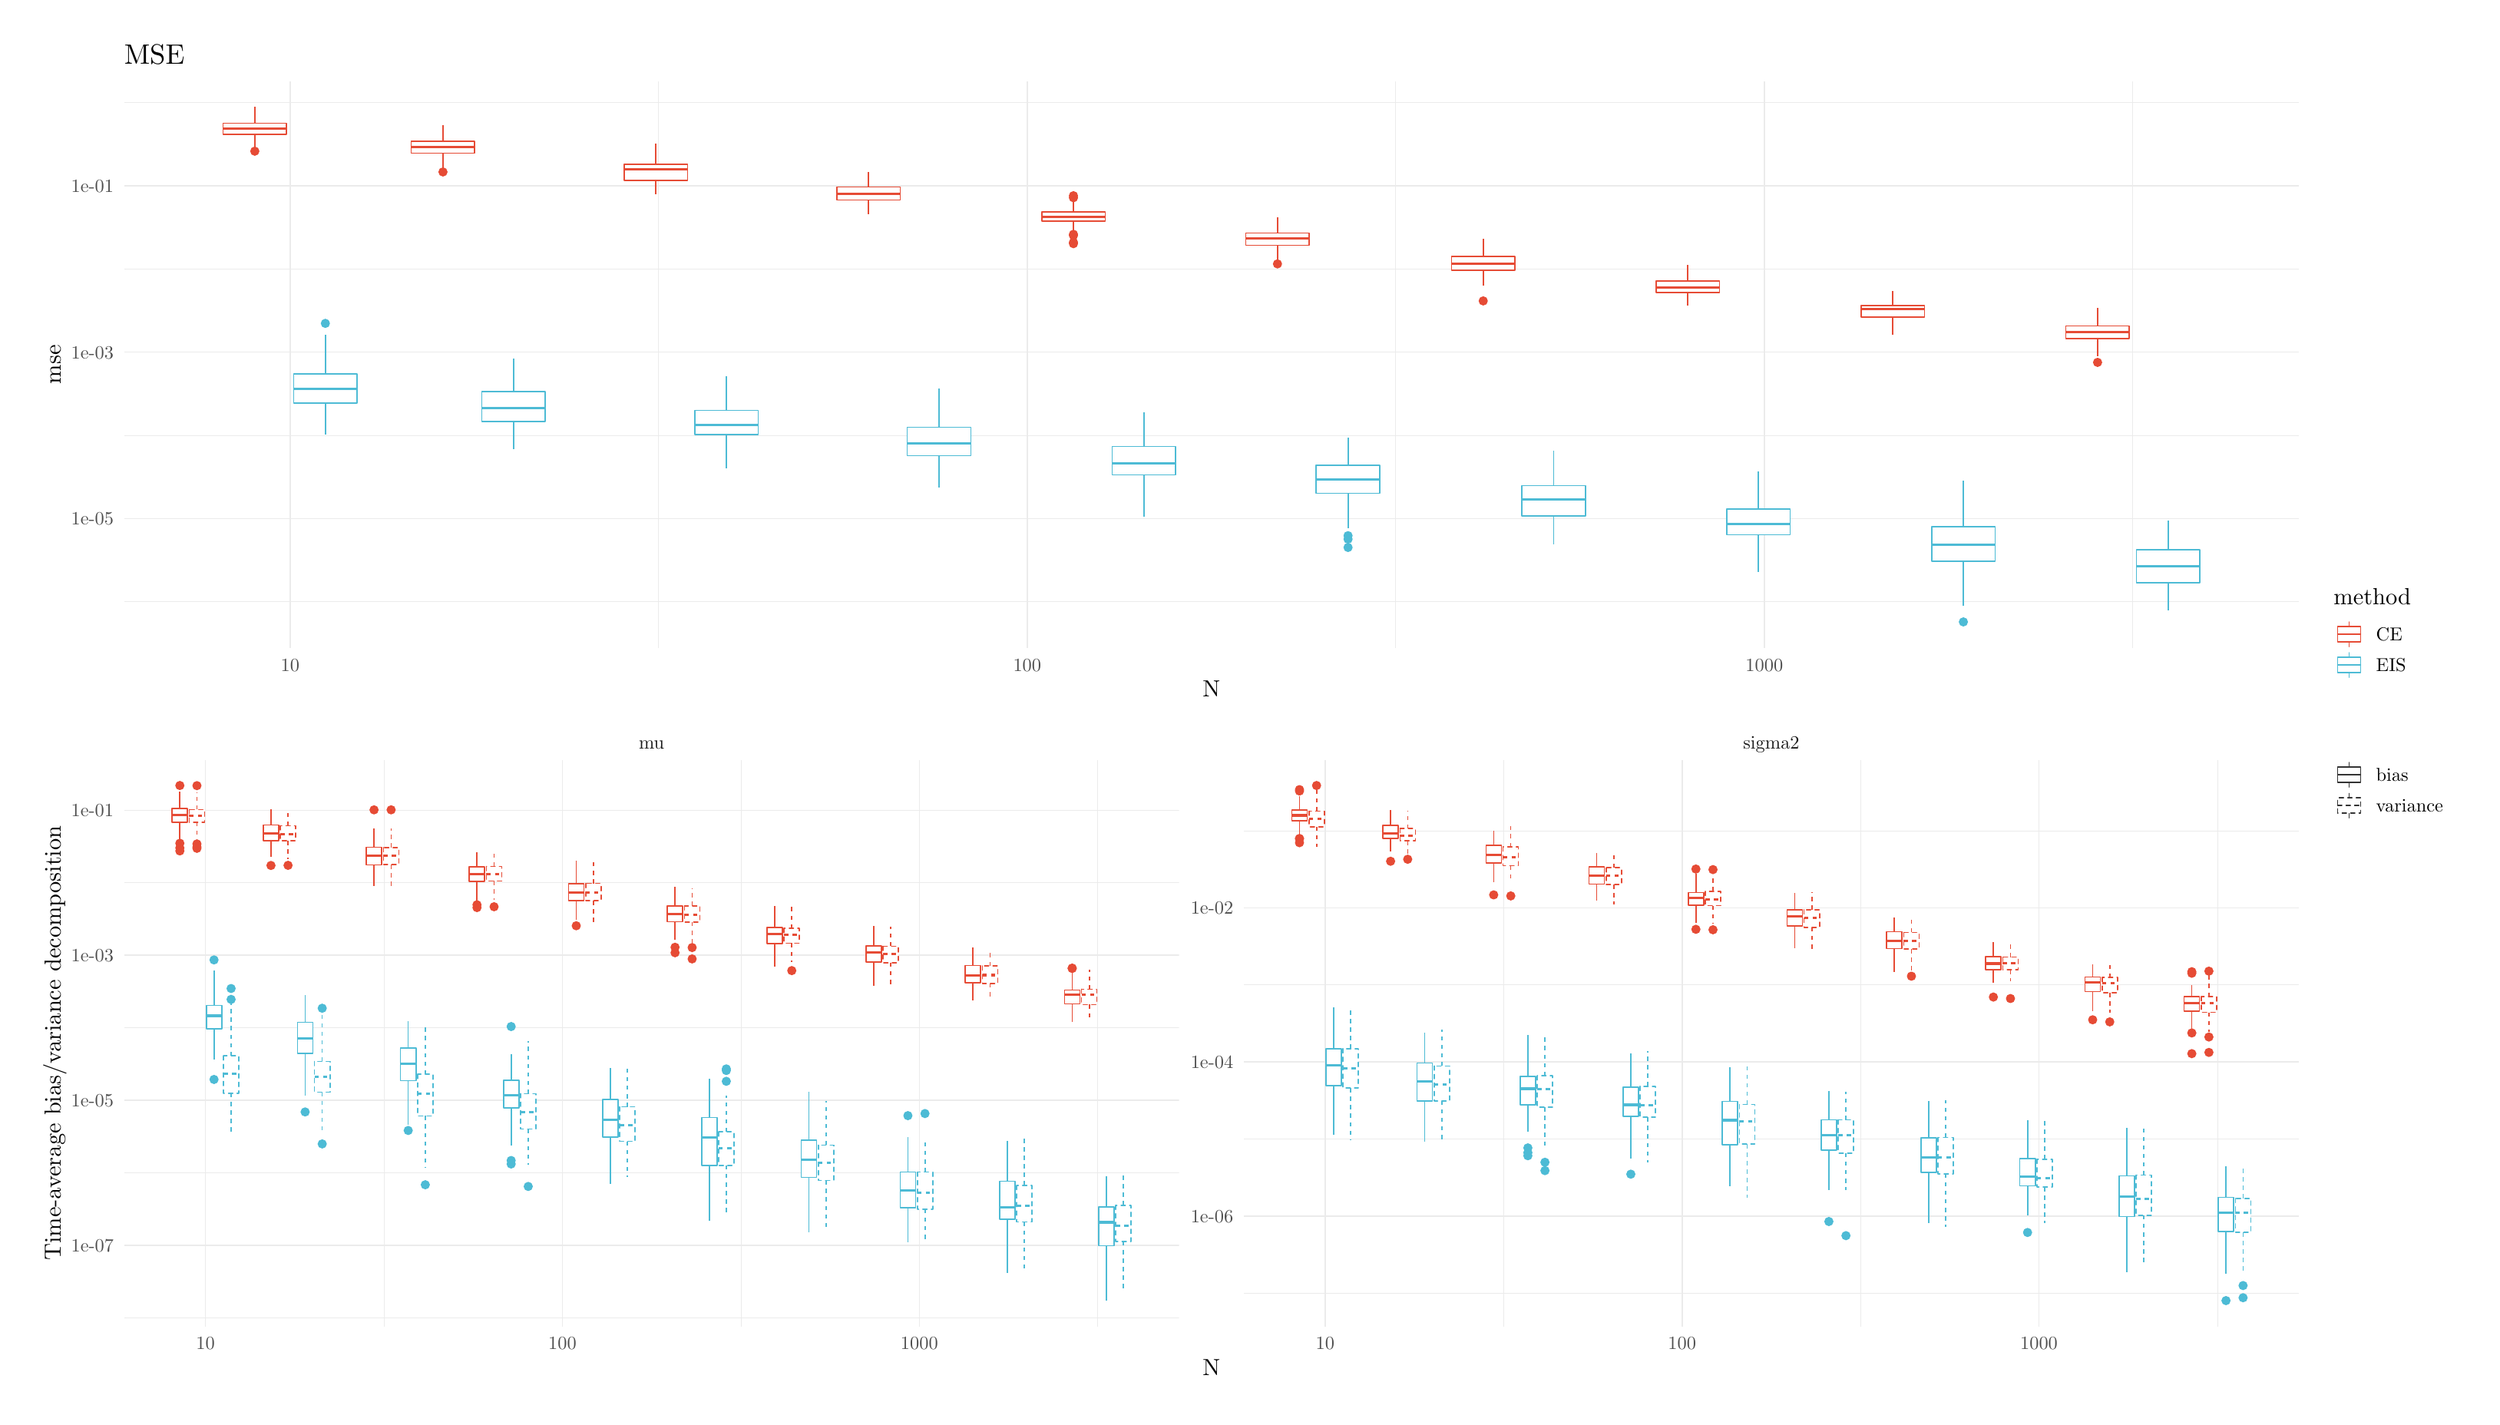
\begin{tikzpicture}[x=1pt,y=1pt]
\definecolor{fillColor}{RGB}{255,255,255}
\path[use as bounding box,fill=fillColor,fill opacity=0.00] (0,0) rectangle (1156.32,650.43);
\begin{scope}
\path[clip] ( 48.45,355.61) rectangle (1071.82,622.27);
\definecolor{drawColor}{gray}{0.92}

\path[draw=drawColor,line width= 0.3pt,line join=round] ( 48.45,377.19) --
	(1071.82,377.19);

\path[draw=drawColor,line width= 0.3pt,line join=round] ( 48.45,455.52) --
	(1071.82,455.52);

\path[draw=drawColor,line width= 0.3pt,line join=round] ( 48.45,533.86) --
	(1071.82,533.86);

\path[draw=drawColor,line width= 0.3pt,line join=round] ( 48.45,612.20) --
	(1071.82,612.20);

\path[draw=drawColor,line width= 0.3pt,line join=round] (299.97,355.61) --
	(299.97,622.27);

\path[draw=drawColor,line width= 0.3pt,line join=round] (646.87,355.61) --
	(646.87,622.27);

\path[draw=drawColor,line width= 0.3pt,line join=round] (993.77,355.61) --
	(993.77,622.27);

\path[draw=drawColor,line width= 0.6pt,line join=round] ( 48.45,416.35) --
	(1071.82,416.35);

\path[draw=drawColor,line width= 0.6pt,line join=round] ( 48.45,494.69) --
	(1071.82,494.69);

\path[draw=drawColor,line width= 0.6pt,line join=round] ( 48.45,573.03) --
	(1071.82,573.03);

\path[draw=drawColor,line width= 0.6pt,line join=round] (126.52,355.61) --
	(126.52,622.27);

\path[draw=drawColor,line width= 0.6pt,line join=round] (473.42,355.61) --
	(473.42,622.27);

\path[draw=drawColor,line width= 0.6pt,line join=round] (820.32,355.61) --
	(820.32,622.27);
\definecolor{drawColor}{RGB}{230,75,53}
\definecolor{fillColor}{RGB}{230,75,53}

\path[draw=drawColor,line width= 0.4pt,line join=round,line cap=round,fill=fillColor] (109.91,589.27) circle (  1.96);

\path[draw=drawColor,line width= 0.6pt,line join=round] (109.91,602.43) -- (109.91,610.15);

\path[draw=drawColor,line width= 0.6pt,line join=round] (109.91,597.18) -- (109.91,589.35);
\definecolor{fillColor}{RGB}{255,255,255}

\path[draw=drawColor,line width= 0.6pt,line join=round,line cap=round,fill=fillColor] ( 94.97,602.43) --
	( 94.97,597.18) --
	(124.86,597.18) --
	(124.86,602.43) --
	( 94.97,602.43) --
	cycle;

\path[draw=drawColor,line width= 1.1pt,line join=round] ( 94.97,599.88) -- (124.86,599.88);
\definecolor{fillColor}{RGB}{230,75,53}

\path[draw=drawColor,line width= 0.4pt,line join=round,line cap=round,fill=fillColor] (198.47,579.50) circle (  1.96);

\path[draw=drawColor,line width= 0.6pt,line join=round] (198.47,594.01) -- (198.47,601.62);

\path[draw=drawColor,line width= 0.6pt,line join=round] (198.47,588.28) -- (198.47,581.12);
\definecolor{fillColor}{RGB}{255,255,255}

\path[draw=drawColor,line width= 0.6pt,line join=round,line cap=round,fill=fillColor] (183.52,594.01) --
	(183.52,588.28) --
	(213.41,588.28) --
	(213.41,594.01) --
	(183.52,594.01) --
	cycle;

\path[draw=drawColor,line width= 1.1pt,line join=round] (183.52,591.17) -- (213.41,591.17);

\path[draw=drawColor,line width= 0.6pt,line join=round] (298.65,583.04) -- (298.65,592.79);

\path[draw=drawColor,line width= 0.6pt,line join=round] (298.65,575.51) -- (298.65,568.86);

\path[draw=drawColor,line width= 0.6pt,line join=round,line cap=round,fill=fillColor] (283.71,583.04) --
	(283.71,575.51) --
	(313.59,575.51) --
	(313.59,583.04) --
	(283.71,583.04) --
	cycle;

\path[draw=drawColor,line width= 1.1pt,line join=round] (283.71,580.63) -- (313.59,580.63);

\path[draw=drawColor,line width= 0.6pt,line join=round] (398.71,572.42) -- (398.71,579.51);

\path[draw=drawColor,line width= 0.6pt,line join=round] (398.71,566.26) -- (398.71,559.75);

\path[draw=drawColor,line width= 0.6pt,line join=round,line cap=round,fill=fillColor] (383.77,572.42) --
	(383.77,566.26) --
	(413.65,566.26) --
	(413.65,572.42) --
	(383.77,572.42) --
	cycle;

\path[draw=drawColor,line width= 1.1pt,line join=round] (383.77,569.10) -- (413.65,569.10);
\definecolor{fillColor}{RGB}{230,75,53}

\path[draw=drawColor,line width= 0.4pt,line join=round,line cap=round,fill=fillColor] (495.18,549.62) circle (  1.96);

\path[draw=drawColor,line width= 0.4pt,line join=round,line cap=round,fill=fillColor] (495.18,568.31) circle (  1.96);

\path[draw=drawColor,line width= 0.4pt,line join=round,line cap=round,fill=fillColor] (495.18,567.37) circle (  1.96);

\path[draw=drawColor,line width= 0.4pt,line join=round,line cap=round,fill=fillColor] (495.18,550.15) circle (  1.96);

\path[draw=drawColor,line width= 0.4pt,line join=round,line cap=round,fill=fillColor] (495.18,546.37) circle (  1.96);

\path[draw=drawColor,line width= 0.4pt,line join=round,line cap=round,fill=fillColor] (495.18,545.75) circle (  1.96);

\path[draw=drawColor,line width= 0.6pt,line join=round] (495.18,560.64) -- (495.18,566.67);

\path[draw=drawColor,line width= 0.6pt,line join=round] (495.18,556.47) -- (495.18,551.07);
\definecolor{fillColor}{RGB}{255,255,255}

\path[draw=drawColor,line width= 0.6pt,line join=round,line cap=round,fill=fillColor] (480.23,560.64) --
	(480.23,556.47) --
	(510.12,556.47) --
	(510.12,560.64) --
	(480.23,560.64) --
	cycle;

\path[draw=drawColor,line width= 1.1pt,line join=round] (480.23,558.41) -- (510.12,558.41);
\definecolor{fillColor}{RGB}{230,75,53}

\path[draw=drawColor,line width= 0.4pt,line join=round,line cap=round,fill=fillColor] (591.20,536.22) circle (  1.96);

\path[draw=drawColor,line width= 0.6pt,line join=round] (591.20,550.79) -- (591.20,558.01);

\path[draw=drawColor,line width= 0.6pt,line join=round] (591.20,545.03) -- (591.20,537.39);
\definecolor{fillColor}{RGB}{255,255,255}

\path[draw=drawColor,line width= 0.6pt,line join=round,line cap=round,fill=fillColor] (576.25,550.79) --
	(576.25,545.03) --
	(606.14,545.03) --
	(606.14,550.79) --
	(576.25,550.79) --
	cycle;

\path[draw=drawColor,line width= 1.1pt,line join=round] (576.25,548.11) -- (606.14,548.11);
\definecolor{fillColor}{RGB}{230,75,53}

\path[draw=drawColor,line width= 0.4pt,line join=round,line cap=round,fill=fillColor] (688.03,518.80) circle (  1.96);

\path[draw=drawColor,line width= 0.6pt,line join=round] (688.03,539.77) -- (688.03,548.16);

\path[draw=drawColor,line width= 0.6pt,line join=round] (688.03,533.22) -- (688.03,525.96);
\definecolor{fillColor}{RGB}{255,255,255}

\path[draw=drawColor,line width= 0.6pt,line join=round,line cap=round,fill=fillColor] (673.08,539.77) --
	(673.08,533.22) --
	(702.97,533.22) --
	(702.97,539.77) --
	(673.08,539.77) --
	cycle;

\path[draw=drawColor,line width= 1.1pt,line join=round] (673.08,536.41) -- (702.97,536.41);

\path[draw=drawColor,line width= 0.6pt,line join=round] (784.28,528.06) -- (784.28,535.76);

\path[draw=drawColor,line width= 0.6pt,line join=round] (784.28,522.86) -- (784.28,516.78);

\path[draw=drawColor,line width= 0.6pt,line join=round,line cap=round,fill=fillColor] (769.34,528.06) --
	(769.34,522.86) --
	(799.23,522.86) --
	(799.23,528.06) --
	(769.34,528.06) --
	cycle;

\path[draw=drawColor,line width= 1.1pt,line join=round] (769.34,525.06) -- (799.23,525.06);

\path[draw=drawColor,line width= 0.6pt,line join=round] (880.79,516.67) -- (880.79,523.61);

\path[draw=drawColor,line width= 0.6pt,line join=round] (880.79,511.12) -- (880.79,502.84);

\path[draw=drawColor,line width= 0.6pt,line join=round,line cap=round,fill=fillColor] (865.85,516.67) --
	(865.85,511.12) --
	(895.73,511.12) --
	(895.73,516.67) --
	(865.85,516.67) --
	cycle;

\path[draw=drawColor,line width= 1.1pt,line join=round] (865.85,514.82) -- (895.73,514.82);
\definecolor{fillColor}{RGB}{230,75,53}

\path[draw=drawColor,line width= 0.4pt,line join=round,line cap=round,fill=fillColor] (977.15,489.87) circle (  1.96);

\path[draw=drawColor,line width= 0.6pt,line join=round] (977.15,507.02) -- (977.15,515.40);

\path[draw=drawColor,line width= 0.6pt,line join=round] (977.15,501.00) -- (977.15,492.74);
\definecolor{fillColor}{RGB}{255,255,255}

\path[draw=drawColor,line width= 0.6pt,line join=round,line cap=round,fill=fillColor] (962.20,507.02) --
	(962.20,501.00) --
	(992.09,501.00) --
	(992.09,507.02) --
	(962.20,507.02) --
	cycle;

\path[draw=drawColor,line width= 1.1pt,line join=round] (962.20,504.08) -- (992.09,504.08);
\definecolor{drawColor}{RGB}{77,187,213}
\definecolor{fillColor}{RGB}{77,187,213}

\path[draw=drawColor,line width= 0.4pt,line join=round,line cap=round,fill=fillColor] (143.12,508.23) circle (  1.96);

\path[draw=drawColor,line width= 0.6pt,line join=round] (143.12,484.52) -- (143.12,502.75);

\path[draw=drawColor,line width= 0.6pt,line join=round] (143.12,470.70) -- (143.12,456.04);
\definecolor{fillColor}{RGB}{255,255,255}

\path[draw=drawColor,line width= 0.6pt,line join=round,line cap=round,fill=fillColor] (128.18,484.52) --
	(128.18,470.70) --
	(158.07,470.70) --
	(158.07,484.52) --
	(128.18,484.52) --
	cycle;

\path[draw=drawColor,line width= 1.1pt,line join=round] (128.18,477.34) -- (158.07,477.34);

\path[draw=drawColor,line width= 0.6pt,line join=round] (231.68,476.16) -- (231.68,491.74);

\path[draw=drawColor,line width= 0.6pt,line join=round] (231.68,461.96) -- (231.68,449.14);

\path[draw=drawColor,line width= 0.6pt,line join=round,line cap=round,fill=fillColor] (216.73,476.16) --
	(216.73,461.96) --
	(246.62,461.96) --
	(246.62,476.16) --
	(216.73,476.16) --
	cycle;

\path[draw=drawColor,line width= 1.1pt,line join=round] (216.73,468.25) -- (246.62,468.25);

\path[draw=drawColor,line width= 0.6pt,line join=round] (331.86,467.34) -- (331.86,483.32);

\path[draw=drawColor,line width= 0.6pt,line join=round] (331.86,455.96) -- (331.86,440.11);

\path[draw=drawColor,line width= 0.6pt,line join=round,line cap=round,fill=fillColor] (316.91,467.34) --
	(316.91,455.96) --
	(346.80,455.96) --
	(346.80,467.34) --
	(316.91,467.34) --
	cycle;

\path[draw=drawColor,line width= 1.1pt,line join=round] (316.91,460.56) -- (346.80,460.56);

\path[draw=drawColor,line width= 0.6pt,line join=round] (431.92,459.29) -- (431.92,477.47);

\path[draw=drawColor,line width= 0.6pt,line join=round] (431.92,446.02) -- (431.92,430.85);

\path[draw=drawColor,line width= 0.6pt,line join=round,line cap=round,fill=fillColor] (416.97,459.29) --
	(416.97,446.02) --
	(446.86,446.02) --
	(446.86,459.29) --
	(416.97,459.29) --
	cycle;

\path[draw=drawColor,line width= 1.1pt,line join=round] (416.97,451.75) -- (446.86,451.75);

\path[draw=drawColor,line width= 0.6pt,line join=round] (528.38,450.25) -- (528.38,466.27);

\path[draw=drawColor,line width= 0.6pt,line join=round] (528.38,436.97) -- (528.38,417.16);

\path[draw=drawColor,line width= 0.6pt,line join=round,line cap=round,fill=fillColor] (513.44,450.25) --
	(513.44,436.97) --
	(543.33,436.97) --
	(543.33,450.25) --
	(513.44,450.25) --
	cycle;

\path[draw=drawColor,line width= 1.1pt,line join=round] (513.44,442.28) -- (543.33,442.28);
\definecolor{fillColor}{RGB}{77,187,213}

\path[draw=drawColor,line width= 0.4pt,line join=round,line cap=round,fill=fillColor] (624.41,406.69) circle (  1.96);

\path[draw=drawColor,line width= 0.4pt,line join=round,line cap=round,fill=fillColor] (624.41,402.77) circle (  1.96);

\path[draw=drawColor,line width= 0.4pt,line join=round,line cap=round,fill=fillColor] (624.41,408.31) circle (  1.96);

\path[draw=drawColor,line width= 0.6pt,line join=round] (624.41,441.40) -- (624.41,454.31);

\path[draw=drawColor,line width= 0.6pt,line join=round] (624.41,428.26) -- (624.41,411.70);
\definecolor{fillColor}{RGB}{255,255,255}

\path[draw=drawColor,line width= 0.6pt,line join=round,line cap=round,fill=fillColor] (609.46,441.40) --
	(609.46,428.26) --
	(639.35,428.26) --
	(639.35,441.40) --
	(609.46,441.40) --
	cycle;

\path[draw=drawColor,line width= 1.1pt,line join=round] (609.46,434.60) -- (639.35,434.60);

\path[draw=drawColor,line width= 0.6pt,line join=round] (721.23,431.86) -- (721.23,448.33);

\path[draw=drawColor,line width= 0.6pt,line join=round] (721.23,417.63) -- (721.23,404.11);

\path[draw=drawColor,line width= 0.6pt,line join=round,line cap=round,fill=fillColor] (706.29,431.86) --
	(706.29,417.63) --
	(736.18,417.63) --
	(736.18,431.86) --
	(706.29,431.86) --
	cycle;

\path[draw=drawColor,line width= 1.1pt,line join=round] (706.29,425.20) -- (736.18,425.20);

\path[draw=drawColor,line width= 0.6pt,line join=round] (817.49,420.78) -- (817.49,438.51);

\path[draw=drawColor,line width= 0.6pt,line join=round] (817.49,408.71) -- (817.49,391.27);

\path[draw=drawColor,line width= 0.6pt,line join=round,line cap=round,fill=fillColor] (802.55,420.78) --
	(802.55,408.71) --
	(832.43,408.71) --
	(832.43,420.78) --
	(802.55,420.78) --
	cycle;

\path[draw=drawColor,line width= 1.1pt,line join=round] (802.55,413.72) -- (832.43,413.72);
\definecolor{fillColor}{RGB}{77,187,213}

\path[draw=drawColor,line width= 0.4pt,line join=round,line cap=round,fill=fillColor] (914.00,367.73) circle (  1.96);

\path[draw=drawColor,line width= 0.6pt,line join=round] (914.00,412.42) -- (914.00,434.20);

\path[draw=drawColor,line width= 0.6pt,line join=round] (914.00,396.33) -- (914.00,375.20);
\definecolor{fillColor}{RGB}{255,255,255}

\path[draw=drawColor,line width= 0.6pt,line join=round,line cap=round,fill=fillColor] (899.06,412.42) --
	(899.06,396.33) --
	(928.94,396.33) --
	(928.94,412.42) --
	(899.06,412.42) --
	cycle;

\path[draw=drawColor,line width= 1.1pt,line join=round] (899.06,404.04) -- (928.94,404.04);

\path[draw=drawColor,line width= 0.6pt,line join=round] (1010.36,401.68) -- (1010.36,415.31);

\path[draw=drawColor,line width= 0.6pt,line join=round] (1010.36,386.17) -- (1010.36,373.01);

\path[draw=drawColor,line width= 0.6pt,line join=round,line cap=round,fill=fillColor] (995.41,401.68) --
	(995.41,386.17) --
	(1025.30,386.17) --
	(1025.30,401.68) --
	(995.41,401.68) --
	cycle;

\path[draw=drawColor,line width= 1.1pt,line join=round] (995.41,393.86) -- (1025.30,393.86);
\end{scope}
\begin{scope}
\path[clip] (  0.00,  0.00) rectangle (1156.32,650.43);
\definecolor{drawColor}{gray}{0.30}

\node[text=drawColor,anchor=base east,inner sep=0pt, outer sep=0pt, scale=  0.88] at ( 43.50,413.32) {1e-05};

\node[text=drawColor,anchor=base east,inner sep=0pt, outer sep=0pt, scale=  0.88] at ( 43.50,491.66) {1e-03};

\node[text=drawColor,anchor=base east,inner sep=0pt, outer sep=0pt, scale=  0.88] at ( 43.50,570.00) {1e-01};
\end{scope}
\begin{scope}
\path[clip] (  0.00,  0.00) rectangle (1156.32,650.43);
\definecolor{drawColor}{gray}{0.30}

\node[text=drawColor,anchor=base,inner sep=0pt, outer sep=0pt, scale=  0.88] at (126.52,344.60) {10};

\node[text=drawColor,anchor=base,inner sep=0pt, outer sep=0pt, scale=  0.88] at (473.42,344.60) {100};

\node[text=drawColor,anchor=base,inner sep=0pt, outer sep=0pt, scale=  0.88] at (820.32,344.60) {1000};
\end{scope}
\begin{scope}
\path[clip] (  0.00,  0.00) rectangle (1156.32,650.43);
\definecolor{drawColor}{RGB}{0,0,0}

\node[text=drawColor,anchor=base,inner sep=0pt, outer sep=0pt, scale=  1.10] at (560.13,332.56) {N};
\end{scope}
\begin{scope}
\path[clip] (  0.00,  0.00) rectangle (1156.32,650.43);
\definecolor{drawColor}{RGB}{0,0,0}

\node[text=drawColor,rotate= 90.00,anchor=base,inner sep=0pt, outer sep=0pt, scale=  1.10] at ( 18.58,488.94) {mse};
\end{scope}
\begin{scope}
\path[clip] (  0.00,  0.00) rectangle (1156.32,650.43);
\definecolor{drawColor}{RGB}{0,0,0}

\node[text=drawColor,anchor=base west,inner sep=0pt, outer sep=0pt, scale=  1.32] at ( 48.45,630.34) {MSE};
\end{scope}
\begin{scope}
\path[clip] ( 48.45, 36.19) rectangle (544.89,302.85);
\definecolor{drawColor}{gray}{0.92}

\path[draw=drawColor,line width= 0.3pt,line join=round] ( 48.45, 40.21) --
	(544.89, 40.21);

\path[draw=drawColor,line width= 0.3pt,line join=round] ( 48.45,108.45) --
	(544.89,108.45);

\path[draw=drawColor,line width= 0.3pt,line join=round] ( 48.45,176.68) --
	(544.89,176.68);

\path[draw=drawColor,line width= 0.3pt,line join=round] ( 48.45,244.91) --
	(544.89,244.91);

\path[draw=drawColor,line width= 0.3pt,line join=round] (170.69, 36.19) --
	(170.69,302.85);

\path[draw=drawColor,line width= 0.3pt,line join=round] (338.67, 36.19) --
	(338.67,302.85);

\path[draw=drawColor,line width= 0.3pt,line join=round] (506.65, 36.19) --
	(506.65,302.85);

\path[draw=drawColor,line width= 0.6pt,line join=round] ( 48.45, 74.33) --
	(544.89, 74.33);

\path[draw=drawColor,line width= 0.6pt,line join=round] ( 48.45,142.56) --
	(544.89,142.56);

\path[draw=drawColor,line width= 0.6pt,line join=round] ( 48.45,210.80) --
	(544.89,210.80);

\path[draw=drawColor,line width= 0.6pt,line join=round] ( 48.45,279.03) --
	(544.89,279.03);

\path[draw=drawColor,line width= 0.6pt,line join=round] ( 86.70, 36.19) --
	( 86.70,302.85);

\path[draw=drawColor,line width= 0.6pt,line join=round] (254.68, 36.19) --
	(254.68,302.85);

\path[draw=drawColor,line width= 0.6pt,line join=round] (422.66, 36.19) --
	(422.66,302.85);
\definecolor{drawColor}{RGB}{230,75,53}
\definecolor{fillColor}{RGB}{230,75,53}

\path[draw=drawColor,line width= 0.4pt,line join=round,line cap=round,fill=fillColor] ( 74.64,290.73) circle (  1.96);

\path[draw=drawColor,line width= 0.4pt,line join=round,line cap=round,fill=fillColor] ( 74.64,259.94) circle (  1.96);

\path[draw=drawColor,line width= 0.4pt,line join=round,line cap=round,fill=fillColor] ( 74.64,263.55) circle (  1.96);

\path[draw=drawColor,line width= 0.4pt,line join=round,line cap=round,fill=fillColor] ( 74.64,261.36) circle (  1.96);

\path[draw=drawColor,line width= 0.6pt,line join=round] ( 74.64,279.83) -- ( 74.64,287.94);

\path[draw=drawColor,line width= 0.6pt,line join=round] ( 74.64,273.38) -- ( 74.64,263.91);
\definecolor{fillColor}{RGB}{255,255,255}

\path[draw=drawColor,line width= 0.6pt,line join=round,line cap=round,fill=fillColor] ( 71.02,279.83) --
	( 71.02,273.38) --
	( 78.26,273.38) --
	( 78.26,279.83) --
	( 71.02,279.83) --
	cycle;

\path[draw=drawColor,line width= 1.1pt,line join=round] ( 71.02,276.71) -- ( 78.26,276.71);
\definecolor{fillColor}{RGB}{230,75,53}

\path[draw=drawColor,line width= 0.4pt,line join=round,line cap=round,fill=fillColor] (117.52,253.10) circle (  1.96);

\path[draw=drawColor,line width= 0.6pt,line join=round] (117.52,272.15) -- (117.52,279.49);

\path[draw=drawColor,line width= 0.6pt,line join=round] (117.52,264.84) -- (117.52,257.32);
\definecolor{fillColor}{RGB}{255,255,255}

\path[draw=drawColor,line width= 0.6pt,line join=round,line cap=round,fill=fillColor] (113.90,272.15) --
	(113.90,264.84) --
	(121.14,264.84) --
	(121.14,272.15) --
	(113.90,272.15) --
	cycle;

\path[draw=drawColor,line width= 1.1pt,line join=round] (113.90,268.24) -- (121.14,268.24);
\definecolor{fillColor}{RGB}{230,75,53}

\path[draw=drawColor,line width= 0.4pt,line join=round,line cap=round,fill=fillColor] (166.03,279.27) circle (  1.96);

\path[draw=drawColor,line width= 0.6pt,line join=round] (166.03,261.68) -- (166.03,270.67);

\path[draw=drawColor,line width= 0.6pt,line join=round] (166.03,253.36) -- (166.03,243.56);
\definecolor{fillColor}{RGB}{255,255,255}

\path[draw=drawColor,line width= 0.6pt,line join=round,line cap=round,fill=fillColor] (162.41,261.68) --
	(162.41,253.36) --
	(169.65,253.36) --
	(169.65,261.68) --
	(162.41,261.68) --
	cycle;

\path[draw=drawColor,line width= 1.1pt,line join=round] (162.41,257.83) -- (169.65,257.83);
\definecolor{fillColor}{RGB}{230,75,53}

\path[draw=drawColor,line width= 0.4pt,line join=round,line cap=round,fill=fillColor] (214.48,233.28) circle (  1.96);

\path[draw=drawColor,line width= 0.4pt,line join=round,line cap=round,fill=fillColor] (214.48,234.60) circle (  1.96);

\path[draw=drawColor,line width= 0.6pt,line join=round] (214.48,252.45) -- (214.48,259.19);

\path[draw=drawColor,line width= 0.6pt,line join=round] (214.48,245.50) -- (214.48,236.52);
\definecolor{fillColor}{RGB}{255,255,255}

\path[draw=drawColor,line width= 0.6pt,line join=round,line cap=round,fill=fillColor] (210.87,252.45) --
	(210.87,245.50) --
	(218.10,245.50) --
	(218.10,252.45) --
	(210.87,252.45) --
	cycle;

\path[draw=drawColor,line width= 1.1pt,line join=round] (210.87,248.89) -- (218.10,248.89);
\definecolor{fillColor}{RGB}{230,75,53}

\path[draw=drawColor,line width= 0.4pt,line join=round,line cap=round,fill=fillColor] (261.20,224.72) circle (  1.96);

\path[draw=drawColor,line width= 0.6pt,line join=round] (261.20,244.46) -- (261.20,255.34);

\path[draw=drawColor,line width= 0.6pt,line join=round] (261.20,236.68) -- (261.20,227.57);
\definecolor{fillColor}{RGB}{255,255,255}

\path[draw=drawColor,line width= 0.6pt,line join=round,line cap=round,fill=fillColor] (257.58,244.46) --
	(257.58,236.68) --
	(264.81,236.68) --
	(264.81,244.46) --
	(257.58,244.46) --
	cycle;

\path[draw=drawColor,line width= 1.1pt,line join=round] (257.58,240.28) -- (264.81,240.28);
\definecolor{fillColor}{RGB}{230,75,53}

\path[draw=drawColor,line width= 0.4pt,line join=round,line cap=round,fill=fillColor] (307.69,212.03) circle (  1.96);

\path[draw=drawColor,line width= 0.4pt,line join=round,line cap=round,fill=fillColor] (307.69,214.60) circle (  1.96);

\path[draw=drawColor,line width= 0.6pt,line join=round] (307.69,234.13) -- (307.69,242.93);

\path[draw=drawColor,line width= 0.6pt,line join=round] (307.69,226.67) -- (307.69,218.03);
\definecolor{fillColor}{RGB}{255,255,255}

\path[draw=drawColor,line width= 0.6pt,line join=round,line cap=round,fill=fillColor] (304.08,234.13) --
	(304.08,226.67) --
	(311.31,226.67) --
	(311.31,234.13) --
	(304.08,234.13) --
	cycle;

\path[draw=drawColor,line width= 1.1pt,line join=round] (304.08,230.28) -- (311.31,230.28);

\path[draw=drawColor,line width= 0.6pt,line join=round] (354.58,223.99) -- (354.58,233.89);

\path[draw=drawColor,line width= 0.6pt,line join=round] (354.58,216.38) -- (354.58,205.43);

\path[draw=drawColor,line width= 0.6pt,line join=round,line cap=round,fill=fillColor] (350.96,223.99) --
	(350.96,216.38) --
	(358.20,216.38) --
	(358.20,223.99) --
	(350.96,223.99) --
	cycle;

\path[draw=drawColor,line width= 1.1pt,line join=round] (350.96,220.73) -- (358.20,220.73);

\path[draw=drawColor,line width= 0.6pt,line join=round] (401.19,215.33) -- (401.19,224.51);

\path[draw=drawColor,line width= 0.6pt,line join=round] (401.19,207.61) -- (401.19,196.40);

\path[draw=drawColor,line width= 0.6pt,line join=round,line cap=round,fill=fillColor] (397.57,215.33) --
	(397.57,207.61) --
	(404.81,207.61) --
	(404.81,215.33) --
	(397.57,215.33) --
	cycle;

\path[draw=drawColor,line width= 1.1pt,line join=round] (397.57,212.04) -- (404.81,212.04);

\path[draw=drawColor,line width= 0.6pt,line join=round] (447.93,206.05) -- (447.93,214.43);

\path[draw=drawColor,line width= 0.6pt,line join=round] (447.93,198.01) -- (447.93,189.49);

\path[draw=drawColor,line width= 0.6pt,line join=round,line cap=round,fill=fillColor] (444.31,206.05) --
	(444.31,198.01) --
	(451.54,198.01) --
	(451.54,206.05) --
	(444.31,206.05) --
	cycle;

\path[draw=drawColor,line width= 1.1pt,line join=round] (444.31,201.25) -- (451.54,201.25);
\definecolor{fillColor}{RGB}{230,75,53}

\path[draw=drawColor,line width= 0.4pt,line join=round,line cap=round,fill=fillColor] (494.59,204.79) circle (  1.96);

\path[draw=drawColor,line width= 0.4pt,line join=round,line cap=round,fill=fillColor] (494.59,204.64) circle (  1.96);

\path[draw=drawColor,line width= 0.6pt,line join=round] (494.59,194.44) -- (494.59,203.20);

\path[draw=drawColor,line width= 0.6pt,line join=round] (494.59,188.00) -- (494.59,179.61);
\definecolor{fillColor}{RGB}{255,255,255}

\path[draw=drawColor,line width= 0.6pt,line join=round,line cap=round,fill=fillColor] (490.97,194.44) --
	(490.97,188.00) --
	(498.20,188.00) --
	(498.20,194.44) --
	(490.97,194.44) --
	cycle;

\path[draw=drawColor,line width= 1.1pt,line join=round] (490.97,192.28) -- (498.20,192.28);
\definecolor{fillColor}{RGB}{230,75,53}

\path[draw=drawColor,line width= 0.4pt,line join=round,line cap=round,fill=fillColor] ( 82.68,290.67) circle (  1.96);

\path[draw=drawColor,line width= 0.4pt,line join=round,line cap=round,fill=fillColor] ( 82.68,261.17) circle (  1.96);

\path[draw=drawColor,line width= 0.4pt,line join=round,line cap=round,fill=fillColor] ( 82.68,263.24) circle (  1.96);

\path[draw=drawColor,line width= 0.4pt,line join=round,line cap=round,fill=fillColor] ( 82.68,261.78) circle (  1.96);

\path[draw=drawColor,line width= 0.6pt,dash pattern=on 2pt off 2pt ,line join=round] ( 82.68,279.43) -- ( 82.68,287.44);

\path[draw=drawColor,line width= 0.6pt,dash pattern=on 2pt off 2pt ,line join=round] ( 82.68,273.46) -- ( 82.68,264.54);
\definecolor{fillColor}{RGB}{255,255,255}

\path[draw=drawColor,line width= 0.6pt,dash pattern=on 2pt off 2pt ,line join=round,line cap=round,fill=fillColor] ( 79.06,279.43) --
	( 79.06,273.46) --
	( 86.30,273.46) --
	( 86.30,279.43) --
	( 79.06,279.43) --
	cycle;

\path[draw=drawColor,line width= 1.1pt,dash pattern=on 2pt off 2pt ,line join=round] ( 79.06,276.46) -- ( 86.30,276.46);
\definecolor{fillColor}{RGB}{230,75,53}

\path[draw=drawColor,line width= 0.4pt,line join=round,line cap=round,fill=fillColor] (125.56,253.16) circle (  1.96);

\path[draw=drawColor,line width= 0.6pt,dash pattern=on 2pt off 2pt ,line join=round] (125.56,271.80) -- (125.56,279.39);

\path[draw=drawColor,line width= 0.6pt,dash pattern=on 2pt off 2pt ,line join=round] (125.56,264.71) -- (125.56,256.05);
\definecolor{fillColor}{RGB}{255,255,255}

\path[draw=drawColor,line width= 0.6pt,dash pattern=on 2pt off 2pt ,line join=round,line cap=round,fill=fillColor] (121.94,271.80) --
	(121.94,264.71) --
	(129.18,264.71) --
	(129.18,271.80) --
	(121.94,271.80) --
	cycle;

\path[draw=drawColor,line width= 1.1pt,dash pattern=on 2pt off 2pt ,line join=round] (121.94,267.87) -- (129.18,267.87);
\definecolor{fillColor}{RGB}{230,75,53}

\path[draw=drawColor,line width= 0.4pt,line join=round,line cap=round,fill=fillColor] (174.07,279.28) circle (  1.96);

\path[draw=drawColor,line width= 0.6pt,dash pattern=on 2pt off 2pt ,line join=round] (174.07,261.55) -- (174.07,270.46);

\path[draw=drawColor,line width= 0.6pt,dash pattern=on 2pt off 2pt ,line join=round] (174.07,253.52) -- (174.07,242.85);
\definecolor{fillColor}{RGB}{255,255,255}

\path[draw=drawColor,line width= 0.6pt,dash pattern=on 2pt off 2pt ,line join=round,line cap=round,fill=fillColor] (170.45,261.55) --
	(170.45,253.52) --
	(177.69,253.52) --
	(177.69,261.55) --
	(170.45,261.55) --
	cycle;

\path[draw=drawColor,line width= 1.1pt,dash pattern=on 2pt off 2pt ,line join=round] (170.45,257.64) -- (177.69,257.64);
\definecolor{fillColor}{RGB}{230,75,53}

\path[draw=drawColor,line width= 0.4pt,line join=round,line cap=round,fill=fillColor] (222.52,233.68) circle (  1.96);

\path[draw=drawColor,line width= 0.6pt,dash pattern=on 2pt off 2pt ,line join=round] (222.52,252.64) -- (222.52,259.52);

\path[draw=drawColor,line width= 0.6pt,dash pattern=on 2pt off 2pt ,line join=round] (222.52,245.82) -- (222.52,236.94);
\definecolor{fillColor}{RGB}{255,255,255}

\path[draw=drawColor,line width= 0.6pt,dash pattern=on 2pt off 2pt ,line join=round,line cap=round,fill=fillColor] (218.91,252.64) --
	(218.91,245.82) --
	(226.14,245.82) --
	(226.14,252.64) --
	(218.91,252.64) --
	cycle;

\path[draw=drawColor,line width= 1.1pt,dash pattern=on 2pt off 2pt ,line join=round] (218.91,249.03) -- (226.14,249.03);

\path[draw=drawColor,line width= 0.6pt,dash pattern=on 2pt off 2pt ,line join=round] (269.24,244.65) -- (269.24,254.67);

\path[draw=drawColor,line width= 0.6pt,dash pattern=on 2pt off 2pt ,line join=round] (269.24,236.54) -- (269.24,224.63);

\path[draw=drawColor,line width= 0.6pt,dash pattern=on 2pt off 2pt ,line join=round,line cap=round,fill=fillColor] (265.62,244.65) --
	(265.62,236.54) --
	(272.85,236.54) --
	(272.85,244.65) --
	(265.62,244.65) --
	cycle;

\path[draw=drawColor,line width= 1.1pt,dash pattern=on 2pt off 2pt ,line join=round] (265.62,240.48) -- (272.85,240.48);
\definecolor{fillColor}{RGB}{230,75,53}

\path[draw=drawColor,line width= 0.4pt,line join=round,line cap=round,fill=fillColor] (315.73,209.12) circle (  1.96);

\path[draw=drawColor,line width= 0.4pt,line join=round,line cap=round,fill=fillColor] (315.73,214.46) circle (  1.96);

\path[draw=drawColor,line width= 0.6pt,dash pattern=on 2pt off 2pt ,line join=round] (315.73,234.15) -- (315.73,242.43);

\path[draw=drawColor,line width= 0.6pt,dash pattern=on 2pt off 2pt ,line join=round] (315.73,226.47) -- (315.73,216.36);
\definecolor{fillColor}{RGB}{255,255,255}

\path[draw=drawColor,line width= 0.6pt,dash pattern=on 2pt off 2pt ,line join=round,line cap=round,fill=fillColor] (312.12,234.15) --
	(312.12,226.47) --
	(319.35,226.47) --
	(319.35,234.15) --
	(312.12,234.15) --
	cycle;

\path[draw=drawColor,line width= 1.1pt,dash pattern=on 2pt off 2pt ,line join=round] (312.12,229.92) -- (319.35,229.92);
\definecolor{fillColor}{RGB}{230,75,53}

\path[draw=drawColor,line width= 0.4pt,line join=round,line cap=round,fill=fillColor] (362.62,203.62) circle (  1.96);

\path[draw=drawColor,line width= 0.6pt,dash pattern=on 2pt off 2pt ,line join=round] (362.62,223.51) -- (362.62,233.83);

\path[draw=drawColor,line width= 0.6pt,dash pattern=on 2pt off 2pt ,line join=round] (362.62,216.53) -- (362.62,207.74);
\definecolor{fillColor}{RGB}{255,255,255}

\path[draw=drawColor,line width= 0.6pt,dash pattern=on 2pt off 2pt ,line join=round,line cap=round,fill=fillColor] (359.00,223.51) --
	(359.00,216.53) --
	(366.24,216.53) --
	(366.24,223.51) --
	(359.00,223.51) --
	cycle;

\path[draw=drawColor,line width= 1.1pt,dash pattern=on 2pt off 2pt ,line join=round] (359.00,220.65) -- (366.24,220.65);

\path[draw=drawColor,line width= 0.6pt,dash pattern=on 2pt off 2pt ,line join=round] (409.23,215.08) -- (409.23,224.39);

\path[draw=drawColor,line width= 0.6pt,dash pattern=on 2pt off 2pt ,line join=round] (409.23,207.35) -- (409.23,196.83);

\path[draw=drawColor,line width= 0.6pt,dash pattern=on 2pt off 2pt ,line join=round,line cap=round,fill=fillColor] (405.61,215.08) --
	(405.61,207.35) --
	(412.85,207.35) --
	(412.85,215.08) --
	(405.61,215.08) --
	cycle;

\path[draw=drawColor,line width= 1.1pt,dash pattern=on 2pt off 2pt ,line join=round] (405.61,211.62) -- (412.85,211.62);

\path[draw=drawColor,line width= 0.6pt,dash pattern=on 2pt off 2pt ,line join=round] (455.97,205.82) -- (455.97,213.74);

\path[draw=drawColor,line width= 0.6pt,dash pattern=on 2pt off 2pt ,line join=round] (455.97,197.57) -- (455.97,190.82);

\path[draw=drawColor,line width= 0.6pt,dash pattern=on 2pt off 2pt ,line join=round,line cap=round,fill=fillColor] (452.35,205.82) --
	(452.35,197.57) --
	(459.58,197.57) --
	(459.58,205.82) --
	(452.35,205.82) --
	cycle;

\path[draw=drawColor,line width= 1.1pt,dash pattern=on 2pt off 2pt ,line join=round] (452.35,201.51) -- (459.58,201.51);

\path[draw=drawColor,line width= 0.6pt,dash pattern=on 2pt off 2pt ,line join=round] (502.63,194.87) -- (502.63,204.15);

\path[draw=drawColor,line width= 0.6pt,dash pattern=on 2pt off 2pt ,line join=round] (502.63,187.61) -- (502.63,179.99);

\path[draw=drawColor,line width= 0.6pt,dash pattern=on 2pt off 2pt ,line join=round,line cap=round,fill=fillColor] (499.01,194.87) --
	(499.01,187.61) --
	(506.24,187.61) --
	(506.24,194.87) --
	(499.01,194.87) --
	cycle;

\path[draw=drawColor,line width= 1.1pt,dash pattern=on 2pt off 2pt ,line join=round] (499.01,192.34) -- (506.24,192.34);
\definecolor{drawColor}{RGB}{77,187,213}
\definecolor{fillColor}{RGB}{77,187,213}

\path[draw=drawColor,line width= 0.4pt,line join=round,line cap=round,fill=fillColor] ( 90.72,152.39) circle (  1.96);

\path[draw=drawColor,line width= 0.4pt,line join=round,line cap=round,fill=fillColor] ( 90.72,208.65) circle (  1.96);

\path[draw=drawColor,line width= 0.6pt,line join=round] ( 90.72,187.19) -- ( 90.72,203.53);

\path[draw=drawColor,line width= 0.6pt,line join=round] ( 90.72,176.20) -- ( 90.72,161.70);
\definecolor{fillColor}{RGB}{255,255,255}

\path[draw=drawColor,line width= 0.6pt,line join=round,line cap=round,fill=fillColor] ( 87.10,187.19) --
	( 87.10,176.20) --
	( 94.34,176.20) --
	( 94.34,187.19) --
	( 87.10,187.19) --
	cycle;

\path[draw=drawColor,line width= 1.1pt,line join=round] ( 87.10,182.36) -- ( 94.34,182.36);
\definecolor{fillColor}{RGB}{77,187,213}

\path[draw=drawColor,line width= 0.4pt,line join=round,line cap=round,fill=fillColor] (133.60,137.10) circle (  1.96);

\path[draw=drawColor,line width= 0.6pt,line join=round] (133.60,179.25) -- (133.60,192.09);

\path[draw=drawColor,line width= 0.6pt,line join=round] (133.60,164.68) -- (133.60,144.66);
\definecolor{fillColor}{RGB}{255,255,255}

\path[draw=drawColor,line width= 0.6pt,line join=round,line cap=round,fill=fillColor] (129.98,179.25) --
	(129.98,164.68) --
	(137.22,164.68) --
	(137.22,179.25) --
	(129.98,179.25) --
	cycle;

\path[draw=drawColor,line width= 1.1pt,line join=round] (129.98,171.68) -- (137.22,171.68);
\definecolor{fillColor}{RGB}{77,187,213}

\path[draw=drawColor,line width= 0.4pt,line join=round,line cap=round,fill=fillColor] (182.11,128.38) circle (  1.96);

\path[draw=drawColor,line width= 0.6pt,line join=round] (182.11,167.23) -- (182.11,179.78);

\path[draw=drawColor,line width= 0.6pt,line join=round] (182.11,151.86) -- (182.11,131.17);
\definecolor{fillColor}{RGB}{255,255,255}

\path[draw=drawColor,line width= 0.6pt,line join=round,line cap=round,fill=fillColor] (178.49,167.23) --
	(178.49,151.86) --
	(185.73,151.86) --
	(185.73,167.23) --
	(178.49,167.23) --
	cycle;

\path[draw=drawColor,line width= 1.1pt,line join=round] (178.49,159.66) -- (185.73,159.66);
\definecolor{fillColor}{RGB}{77,187,213}

\path[draw=drawColor,line width= 0.4pt,line join=round,line cap=round,fill=fillColor] (230.56,114.25) circle (  1.96);

\path[draw=drawColor,line width= 0.4pt,line join=round,line cap=round,fill=fillColor] (230.56,177.29) circle (  1.96);

\path[draw=drawColor,line width= 0.4pt,line join=round,line cap=round,fill=fillColor] (230.56,112.60) circle (  1.96);

\path[draw=drawColor,line width= 0.6pt,line join=round] (230.56,152.00) -- (230.56,164.22);

\path[draw=drawColor,line width= 0.6pt,line join=round] (230.56,138.95) -- (230.56,121.16);
\definecolor{fillColor}{RGB}{255,255,255}

\path[draw=drawColor,line width= 0.6pt,line join=round,line cap=round,fill=fillColor] (226.95,152.00) --
	(226.95,138.95) --
	(234.18,138.95) --
	(234.18,152.00) --
	(226.95,152.00) --
	cycle;

\path[draw=drawColor,line width= 1.1pt,line join=round] (226.95,144.86) -- (234.18,144.86);

\path[draw=drawColor,line width= 0.6pt,line join=round] (277.28,142.93) -- (277.28,157.92);

\path[draw=drawColor,line width= 0.6pt,line join=round] (277.28,125.29) -- (277.28,103.34);

\path[draw=drawColor,line width= 0.6pt,line join=round,line cap=round,fill=fillColor] (273.66,142.93) --
	(273.66,125.29) --
	(280.90,125.29) --
	(280.90,142.93) --
	(273.66,142.93) --
	cycle;

\path[draw=drawColor,line width= 1.1pt,line join=round] (273.66,133.57) -- (280.90,133.57);

\path[draw=drawColor,line width= 0.6pt,line join=round] (323.77,134.43) -- (323.77,152.66);

\path[draw=drawColor,line width= 0.6pt,line join=round] (323.77,111.92) -- (323.77, 85.88);

\path[draw=drawColor,line width= 0.6pt,line join=round,line cap=round,fill=fillColor] (320.16,134.43) --
	(320.16,111.92) --
	(327.39,111.92) --
	(327.39,134.43) --
	(320.16,134.43) --
	cycle;

\path[draw=drawColor,line width= 1.1pt,line join=round] (320.16,125.21) -- (327.39,125.21);

\path[draw=drawColor,line width= 0.6pt,line join=round] (370.66,123.90) -- (370.66,146.49);

\path[draw=drawColor,line width= 0.6pt,line join=round] (370.66,106.33) -- (370.66, 80.55);

\path[draw=drawColor,line width= 0.6pt,line join=round,line cap=round,fill=fillColor] (367.04,123.90) --
	(367.04,106.33) --
	(374.28,106.33) --
	(374.28,123.90) --
	(367.04,123.90) --
	cycle;

\path[draw=drawColor,line width= 1.1pt,line join=round] (367.04,114.72) -- (374.28,114.72);
\definecolor{fillColor}{RGB}{77,187,213}

\path[draw=drawColor,line width= 0.4pt,line join=round,line cap=round,fill=fillColor] (417.27,135.36) circle (  1.96);

\path[draw=drawColor,line width= 0.6pt,line join=round] (417.27,108.83) -- (417.27,125.33);

\path[draw=drawColor,line width= 0.6pt,line join=round] (417.27, 92.08) -- (417.27, 75.75);
\definecolor{fillColor}{RGB}{255,255,255}

\path[draw=drawColor,line width= 0.6pt,line join=round,line cap=round,fill=fillColor] (413.65,108.83) --
	(413.65, 92.08) --
	(420.89, 92.08) --
	(420.89,108.83) --
	(413.65,108.83) --
	cycle;

\path[draw=drawColor,line width= 1.1pt,line join=round] (413.65,100.13) -- (420.89,100.13);

\path[draw=drawColor,line width= 0.6pt,line join=round] (464.01,104.47) -- (464.01,123.47);

\path[draw=drawColor,line width= 0.6pt,line join=round] (464.01, 86.50) -- (464.01, 61.37);

\path[draw=drawColor,line width= 0.6pt,line join=round,line cap=round,fill=fillColor] (460.39,104.47) --
	(460.39, 86.50) --
	(467.62, 86.50) --
	(467.62,104.47) --
	(460.39,104.47) --
	cycle;

\path[draw=drawColor,line width= 1.1pt,line join=round] (460.39, 92.27) -- (467.62, 92.27);

\path[draw=drawColor,line width= 0.6pt,line join=round] (510.67, 92.47) -- (510.67,106.86);

\path[draw=drawColor,line width= 0.6pt,line join=round] (510.67, 74.13) -- (510.67, 48.31);

\path[draw=drawColor,line width= 0.6pt,line join=round,line cap=round,fill=fillColor] (507.05, 92.47) --
	(507.05, 74.13) --
	(514.28, 74.13) --
	(514.28, 92.47) --
	(507.05, 92.47) --
	cycle;

\path[draw=drawColor,line width= 1.1pt,line join=round] (507.05, 85.16) -- (514.28, 85.16);
\definecolor{fillColor}{RGB}{77,187,213}

\path[draw=drawColor,line width= 0.4pt,line join=round,line cap=round,fill=fillColor] ( 98.76,195.20) circle (  1.96);

\path[draw=drawColor,line width= 0.4pt,line join=round,line cap=round,fill=fillColor] ( 98.76,190.07) circle (  1.96);

\path[draw=drawColor,line width= 0.6pt,dash pattern=on 2pt off 2pt ,line join=round] ( 98.76,163.49) -- ( 98.76,189.70);

\path[draw=drawColor,line width= 0.6pt,dash pattern=on 2pt off 2pt ,line join=round] ( 98.76,145.89) -- ( 98.76,126.69);
\definecolor{fillColor}{RGB}{255,255,255}

\path[draw=drawColor,line width= 0.6pt,dash pattern=on 2pt off 2pt ,line join=round,line cap=round,fill=fillColor] ( 95.14,163.49) --
	( 95.14,145.89) --
	(102.38,145.89) --
	(102.38,163.49) --
	( 95.14,163.49) --
	cycle;

\path[draw=drawColor,line width= 1.1pt,dash pattern=on 2pt off 2pt ,line join=round] ( 95.14,155.15) -- (102.38,155.15);
\definecolor{fillColor}{RGB}{77,187,213}

\path[draw=drawColor,line width= 0.4pt,line join=round,line cap=round,fill=fillColor] (141.64,122.05) circle (  1.96);

\path[draw=drawColor,line width= 0.4pt,line join=round,line cap=round,fill=fillColor] (141.64,185.91) circle (  1.96);

\path[draw=drawColor,line width= 0.6pt,dash pattern=on 2pt off 2pt ,line join=round] (141.64,160.89) -- (141.64,182.64);

\path[draw=drawColor,line width= 0.6pt,dash pattern=on 2pt off 2pt ,line join=round] (141.64,146.38) -- (141.64,127.31);
\definecolor{fillColor}{RGB}{255,255,255}

\path[draw=drawColor,line width= 0.6pt,dash pattern=on 2pt off 2pt ,line join=round,line cap=round,fill=fillColor] (138.02,160.89) --
	(138.02,146.38) --
	(145.26,146.38) --
	(145.26,160.89) --
	(138.02,160.89) --
	cycle;

\path[draw=drawColor,line width= 1.1pt,dash pattern=on 2pt off 2pt ,line join=round] (138.02,153.52) -- (145.26,153.52);
\definecolor{fillColor}{RGB}{77,187,213}

\path[draw=drawColor,line width= 0.4pt,line join=round,line cap=round,fill=fillColor] (190.15,102.83) circle (  1.96);

\path[draw=drawColor,line width= 0.6pt,dash pattern=on 2pt off 2pt ,line join=round] (190.15,154.79) -- (190.15,178.49);

\path[draw=drawColor,line width= 0.6pt,dash pattern=on 2pt off 2pt ,line join=round] (190.15,135.25) -- (190.15,111.21);
\definecolor{fillColor}{RGB}{255,255,255}

\path[draw=drawColor,line width= 0.6pt,dash pattern=on 2pt off 2pt ,line join=round,line cap=round,fill=fillColor] (186.53,154.79) --
	(186.53,135.25) --
	(193.77,135.25) --
	(193.77,154.79) --
	(186.53,154.79) --
	cycle;

\path[draw=drawColor,line width= 1.1pt,dash pattern=on 2pt off 2pt ,line join=round] (186.53,145.75) -- (193.77,145.75);
\definecolor{fillColor}{RGB}{77,187,213}

\path[draw=drawColor,line width= 0.4pt,line join=round,line cap=round,fill=fillColor] (238.60,102.03) circle (  1.96);

\path[draw=drawColor,line width= 0.6pt,dash pattern=on 2pt off 2pt ,line join=round] (238.60,145.74) -- (238.60,170.32);

\path[draw=drawColor,line width= 0.6pt,dash pattern=on 2pt off 2pt ,line join=round] (238.60,129.06) -- (238.60,112.21);
\definecolor{fillColor}{RGB}{255,255,255}

\path[draw=drawColor,line width= 0.6pt,dash pattern=on 2pt off 2pt ,line join=round,line cap=round,fill=fillColor] (234.99,145.74) --
	(234.99,129.06) --
	(242.22,129.06) --
	(242.22,145.74) --
	(234.99,145.74) --
	cycle;

\path[draw=drawColor,line width= 1.1pt,dash pattern=on 2pt off 2pt ,line join=round] (234.99,136.93) -- (242.22,136.93);

\path[draw=drawColor,line width= 0.6pt,dash pattern=on 2pt off 2pt ,line join=round] (285.32,139.50) -- (285.32,158.11);

\path[draw=drawColor,line width= 0.6pt,dash pattern=on 2pt off 2pt ,line join=round] (285.32,123.25) -- (285.32,106.37);

\path[draw=drawColor,line width= 0.6pt,dash pattern=on 2pt off 2pt ,line join=round,line cap=round,fill=fillColor] (281.70,139.50) --
	(281.70,123.25) --
	(288.94,123.25) --
	(288.94,139.50) --
	(281.70,139.50) --
	cycle;

\path[draw=drawColor,line width= 1.1pt,dash pattern=on 2pt off 2pt ,line join=round] (281.70,130.79) -- (288.94,130.79);
\definecolor{fillColor}{RGB}{77,187,213}

\path[draw=drawColor,line width= 0.4pt,line join=round,line cap=round,fill=fillColor] (331.81,157.36) circle (  1.96);

\path[draw=drawColor,line width= 0.4pt,line join=round,line cap=round,fill=fillColor] (331.81,156.60) circle (  1.96);

\path[draw=drawColor,line width= 0.4pt,line join=round,line cap=round,fill=fillColor] (331.81,151.52) circle (  1.96);

\path[draw=drawColor,line width= 0.6pt,dash pattern=on 2pt off 2pt ,line join=round] (331.81,127.68) -- (331.81,144.86);

\path[draw=drawColor,line width= 0.6pt,dash pattern=on 2pt off 2pt ,line join=round] (331.81,111.95) -- (331.81, 89.02);
\definecolor{fillColor}{RGB}{255,255,255}

\path[draw=drawColor,line width= 0.6pt,dash pattern=on 2pt off 2pt ,line join=round,line cap=round,fill=fillColor] (328.20,127.68) --
	(328.20,111.95) --
	(335.43,111.95) --
	(335.43,127.68) --
	(328.20,127.68) --
	cycle;

\path[draw=drawColor,line width= 1.1pt,dash pattern=on 2pt off 2pt ,line join=round] (328.20,120.12) -- (335.43,120.12);

\path[draw=drawColor,line width= 0.6pt,dash pattern=on 2pt off 2pt ,line join=round] (378.70,121.49) -- (378.70,142.17);

\path[draw=drawColor,line width= 0.6pt,dash pattern=on 2pt off 2pt ,line join=round] (378.70,104.91) -- (378.70, 81.14);

\path[draw=drawColor,line width= 0.6pt,dash pattern=on 2pt off 2pt ,line join=round,line cap=round,fill=fillColor] (375.08,121.49) --
	(375.08,104.91) --
	(382.32,104.91) --
	(382.32,121.49) --
	(375.08,121.49) --
	cycle;

\path[draw=drawColor,line width= 1.1pt,dash pattern=on 2pt off 2pt ,line join=round] (375.08,113.24) -- (382.32,113.24);
\definecolor{fillColor}{RGB}{77,187,213}

\path[draw=drawColor,line width= 0.4pt,line join=round,line cap=round,fill=fillColor] (425.31,136.34) circle (  1.96);

\path[draw=drawColor,line width= 0.6pt,dash pattern=on 2pt off 2pt ,line join=round] (425.31,108.80) -- (425.31,123.58);

\path[draw=drawColor,line width= 0.6pt,dash pattern=on 2pt off 2pt ,line join=round] (425.31, 91.39) -- (425.31, 76.53);
\definecolor{fillColor}{RGB}{255,255,255}

\path[draw=drawColor,line width= 0.6pt,dash pattern=on 2pt off 2pt ,line join=round,line cap=round,fill=fillColor] (421.70,108.80) --
	(421.70, 91.39) --
	(428.93, 91.39) --
	(428.93,108.80) --
	(421.70,108.80) --
	cycle;

\path[draw=drawColor,line width= 1.1pt,dash pattern=on 2pt off 2pt ,line join=round] (421.70, 99.23) -- (428.93, 99.23);

\path[draw=drawColor,line width= 0.6pt,dash pattern=on 2pt off 2pt ,line join=round] (472.05,102.51) -- (472.05,125.24);

\path[draw=drawColor,line width= 0.6pt,dash pattern=on 2pt off 2pt ,line join=round] (472.05, 85.34) -- (472.05, 62.82);

\path[draw=drawColor,line width= 0.6pt,dash pattern=on 2pt off 2pt ,line join=round,line cap=round,fill=fillColor] (468.43,102.51) --
	(468.43, 85.34) --
	(475.67, 85.34) --
	(475.67,102.51) --
	(468.43,102.51) --
	cycle;

\path[draw=drawColor,line width= 1.1pt,dash pattern=on 2pt off 2pt ,line join=round] (468.43, 93.08) -- (475.67, 93.08);

\path[draw=drawColor,line width= 0.6pt,dash pattern=on 2pt off 2pt ,line join=round] (518.71, 93.19) -- (518.71,108.51);

\path[draw=drawColor,line width= 0.6pt,dash pattern=on 2pt off 2pt ,line join=round] (518.71, 76.16) -- (518.71, 53.55);

\path[draw=drawColor,line width= 0.6pt,dash pattern=on 2pt off 2pt ,line join=round,line cap=round,fill=fillColor] (515.09, 93.19) --
	(515.09, 76.16) --
	(522.32, 76.16) --
	(522.32, 93.19) --
	(515.09, 93.19) --
	cycle;

\path[draw=drawColor,line width= 1.1pt,dash pattern=on 2pt off 2pt ,line join=round] (515.09, 83.62) -- (522.32, 83.62);
\end{scope}
\begin{scope}
\path[clip] (575.38, 36.19) rectangle (1071.82,302.85);
\definecolor{drawColor}{gray}{0.92}

\path[draw=drawColor,line width= 0.3pt,line join=round] (575.38, 51.75) --
	(1071.82, 51.75);

\path[draw=drawColor,line width= 0.3pt,line join=round] (575.38,124.32) --
	(1071.82,124.32);

\path[draw=drawColor,line width= 0.3pt,line join=round] (575.38,196.90) --
	(1071.82,196.90);

\path[draw=drawColor,line width= 0.3pt,line join=round] (575.38,269.47) --
	(1071.82,269.47);

\path[draw=drawColor,line width= 0.3pt,line join=round] (697.61, 36.19) --
	(697.61,302.85);

\path[draw=drawColor,line width= 0.3pt,line join=round] (865.60, 36.19) --
	(865.60,302.85);

\path[draw=drawColor,line width= 0.3pt,line join=round] (1033.58, 36.19) --
	(1033.58,302.85);

\path[draw=drawColor,line width= 0.6pt,line join=round] (575.38, 88.04) --
	(1071.82, 88.04);

\path[draw=drawColor,line width= 0.6pt,line join=round] (575.38,160.61) --
	(1071.82,160.61);

\path[draw=drawColor,line width= 0.6pt,line join=round] (575.38,233.18) --
	(1071.82,233.18);

\path[draw=drawColor,line width= 0.6pt,line join=round] (613.62, 36.19) --
	(613.62,302.85);

\path[draw=drawColor,line width= 0.6pt,line join=round] (781.61, 36.19) --
	(781.61,302.85);

\path[draw=drawColor,line width= 0.6pt,line join=round] (949.59, 36.19) --
	(949.59,302.85);
\definecolor{drawColor}{RGB}{230,75,53}
\definecolor{fillColor}{RGB}{230,75,53}

\path[draw=drawColor,line width= 0.4pt,line join=round,line cap=round,fill=fillColor] (601.56,288.14) circle (  1.96);

\path[draw=drawColor,line width= 0.4pt,line join=round,line cap=round,fill=fillColor] (601.56,288.80) circle (  1.96);

\path[draw=drawColor,line width= 0.4pt,line join=round,line cap=round,fill=fillColor] (601.56,265.78) circle (  1.96);

\path[draw=drawColor,line width= 0.4pt,line join=round,line cap=round,fill=fillColor] (601.56,263.82) circle (  1.96);

\path[draw=drawColor,line width= 0.4pt,line join=round,line cap=round,fill=fillColor] (601.56,265.70) circle (  1.96);

\path[draw=drawColor,line width= 0.6pt,line join=round] (601.56,279.26) -- (601.56,285.67);

\path[draw=drawColor,line width= 0.6pt,line join=round] (601.56,274.03) -- (601.56,267.81);
\definecolor{fillColor}{RGB}{255,255,255}

\path[draw=drawColor,line width= 0.6pt,line join=round,line cap=round,fill=fillColor] (597.94,279.26) --
	(597.94,274.03) --
	(605.18,274.03) --
	(605.18,279.26) --
	(597.94,279.26) --
	cycle;

\path[draw=drawColor,line width= 1.1pt,line join=round] (597.94,276.68) -- (605.18,276.68);
\definecolor{fillColor}{RGB}{230,75,53}

\path[draw=drawColor,line width= 0.4pt,line join=round,line cap=round,fill=fillColor] (644.44,255.08) circle (  1.96);

\path[draw=drawColor,line width= 0.6pt,line join=round] (644.44,272.01) -- (644.44,279.06);

\path[draw=drawColor,line width= 0.6pt,line join=round] (644.44,265.75) -- (644.44,259.71);
\definecolor{fillColor}{RGB}{255,255,255}

\path[draw=drawColor,line width= 0.6pt,line join=round,line cap=round,fill=fillColor] (640.83,272.01) --
	(640.83,265.75) --
	(648.06,265.75) --
	(648.06,272.01) --
	(640.83,272.01) --
	cycle;

\path[draw=drawColor,line width= 1.1pt,line join=round] (640.83,268.07) -- (648.06,268.07);
\definecolor{fillColor}{RGB}{230,75,53}

\path[draw=drawColor,line width= 0.4pt,line join=round,line cap=round,fill=fillColor] (692.96,239.26) circle (  1.96);

\path[draw=drawColor,line width= 0.6pt,line join=round] (692.96,262.51) -- (692.96,269.42);

\path[draw=drawColor,line width= 0.6pt,line join=round] (692.96,254.21) -- (692.96,245.19);
\definecolor{fillColor}{RGB}{255,255,255}

\path[draw=drawColor,line width= 0.6pt,line join=round,line cap=round,fill=fillColor] (689.34,262.51) --
	(689.34,254.21) --
	(696.57,254.21) --
	(696.57,262.51) --
	(689.34,262.51) --
	cycle;

\path[draw=drawColor,line width= 1.1pt,line join=round] (689.34,257.98) -- (696.57,257.98);

\path[draw=drawColor,line width= 0.6pt,line join=round] (741.41,252.56) -- (741.41,258.94);

\path[draw=drawColor,line width= 0.6pt,line join=round] (741.41,244.39) -- (741.41,236.61);

\path[draw=drawColor,line width= 0.6pt,line join=round,line cap=round,fill=fillColor] (737.79,252.56) --
	(737.79,244.39) --
	(745.03,244.39) --
	(745.03,252.56) --
	(737.79,252.56) --
	cycle;

\path[draw=drawColor,line width= 1.1pt,line join=round] (737.79,248.24) -- (745.03,248.24);
\definecolor{fillColor}{RGB}{230,75,53}

\path[draw=drawColor,line width= 0.4pt,line join=round,line cap=round,fill=fillColor] (788.12,251.42) circle (  1.96);

\path[draw=drawColor,line width= 0.4pt,line join=round,line cap=round,fill=fillColor] (788.12,223.05) circle (  1.96);

\path[draw=drawColor,line width= 0.6pt,line join=round] (788.12,240.40) -- (788.12,249.30);

\path[draw=drawColor,line width= 0.6pt,line join=round] (788.12,234.28) -- (788.12,226.20);
\definecolor{fillColor}{RGB}{255,255,255}

\path[draw=drawColor,line width= 0.6pt,line join=round,line cap=round,fill=fillColor] (784.50,240.40) --
	(784.50,234.28) --
	(791.74,234.28) --
	(791.74,240.40) --
	(784.50,240.40) --
	cycle;

\path[draw=drawColor,line width= 1.1pt,line join=round] (784.50,237.69) -- (791.74,237.69);

\path[draw=drawColor,line width= 0.6pt,line join=round] (834.62,232.17) -- (834.62,240.31);

\path[draw=drawColor,line width= 0.6pt,line join=round] (834.62,224.58) -- (834.62,214.34);

\path[draw=drawColor,line width= 0.6pt,line join=round,line cap=round,fill=fillColor] (831.00,232.17) --
	(831.00,224.58) --
	(838.24,224.58) --
	(838.24,232.17) --
	(831.00,232.17) --
	cycle;

\path[draw=drawColor,line width= 1.1pt,line join=round] (831.00,229.24) -- (838.24,229.24);

\path[draw=drawColor,line width= 0.6pt,line join=round] (881.51,221.98) -- (881.51,228.54);

\path[draw=drawColor,line width= 0.6pt,line join=round] (881.51,214.00) -- (881.51,202.99);

\path[draw=drawColor,line width= 0.6pt,line join=round,line cap=round,fill=fillColor] (877.89,221.98) --
	(877.89,214.00) --
	(885.13,214.00) --
	(885.13,221.98) --
	(877.89,221.98) --
	cycle;

\path[draw=drawColor,line width= 1.1pt,line join=round] (877.89,217.42) -- (885.13,217.42);
\definecolor{fillColor}{RGB}{230,75,53}

\path[draw=drawColor,line width= 0.4pt,line join=round,line cap=round,fill=fillColor] (928.12,191.17) circle (  1.96);

\path[draw=drawColor,line width= 0.6pt,line join=round] (928.12,210.10) -- (928.12,217.11);

\path[draw=drawColor,line width= 0.6pt,line join=round] (928.12,204.01) -- (928.12,197.77);
\definecolor{fillColor}{RGB}{255,255,255}

\path[draw=drawColor,line width= 0.6pt,line join=round,line cap=round,fill=fillColor] (924.50,210.10) --
	(924.50,204.01) --
	(931.74,204.01) --
	(931.74,210.10) --
	(924.50,210.10) --
	cycle;

\path[draw=drawColor,line width= 1.1pt,line join=round] (924.50,206.93) -- (931.74,206.93);
\definecolor{fillColor}{RGB}{230,75,53}

\path[draw=drawColor,line width= 0.4pt,line join=round,line cap=round,fill=fillColor] (974.85,180.47) circle (  1.96);

\path[draw=drawColor,line width= 0.6pt,line join=round] (974.85,200.62) -- (974.85,206.64);

\path[draw=drawColor,line width= 0.6pt,line join=round] (974.85,193.69) -- (974.85,184.52);
\definecolor{fillColor}{RGB}{255,255,255}

\path[draw=drawColor,line width= 0.6pt,line join=round,line cap=round,fill=fillColor] (971.23,200.62) --
	(971.23,193.69) --
	(978.47,193.69) --
	(978.47,200.62) --
	(971.23,200.62) --
	cycle;

\path[draw=drawColor,line width= 1.1pt,line join=round] (971.23,197.97) -- (978.47,197.97);
\definecolor{fillColor}{RGB}{230,75,53}

\path[draw=drawColor,line width= 0.4pt,line join=round,line cap=round,fill=fillColor] (1021.51,174.28) circle (  1.96);

\path[draw=drawColor,line width= 0.4pt,line join=round,line cap=round,fill=fillColor] (1021.51,202.38) circle (  1.96);

\path[draw=drawColor,line width= 0.4pt,line join=round,line cap=round,fill=fillColor] (1021.51,164.54) circle (  1.96);

\path[draw=drawColor,line width= 0.4pt,line join=round,line cap=round,fill=fillColor] (1021.51,203.10) circle (  1.96);

\path[draw=drawColor,line width= 0.6pt,line join=round] (1021.51,191.37) -- (1021.51,196.94);

\path[draw=drawColor,line width= 0.6pt,line join=round] (1021.51,184.57) -- (1021.51,175.38);
\definecolor{fillColor}{RGB}{255,255,255}

\path[draw=drawColor,line width= 0.6pt,line join=round,line cap=round,fill=fillColor] (1017.89,191.37) --
	(1017.89,184.57) --
	(1025.13,184.57) --
	(1025.13,191.37) --
	(1017.89,191.37) --
	cycle;

\path[draw=drawColor,line width= 1.1pt,line join=round] (1017.89,188.45) -- (1025.13,188.45);
\definecolor{fillColor}{RGB}{230,75,53}

\path[draw=drawColor,line width= 0.4pt,line join=round,line cap=round,fill=fillColor] (609.60,290.73) circle (  1.96);

\path[draw=drawColor,line width= 0.6pt,dash pattern=on 2pt off 2pt ,line join=round] (609.60,278.68) -- (609.60,288.94);

\path[draw=drawColor,line width= 0.6pt,dash pattern=on 2pt off 2pt ,line join=round] (609.60,271.33) -- (609.60,261.94);
\definecolor{fillColor}{RGB}{255,255,255}

\path[draw=drawColor,line width= 0.6pt,dash pattern=on 2pt off 2pt ,line join=round,line cap=round,fill=fillColor] (605.99,278.68) --
	(605.99,271.33) --
	(613.22,271.33) --
	(613.22,278.68) --
	(605.99,278.68) --
	cycle;

\path[draw=drawColor,line width= 1.1pt,dash pattern=on 2pt off 2pt ,line join=round] (605.99,274.94) -- (613.22,274.94);
\definecolor{fillColor}{RGB}{230,75,53}

\path[draw=drawColor,line width= 0.4pt,line join=round,line cap=round,fill=fillColor] (652.48,256.02) circle (  1.96);

\path[draw=drawColor,line width= 0.6pt,dash pattern=on 2pt off 2pt ,line join=round] (652.48,270.46) -- (652.48,278.67);

\path[draw=drawColor,line width= 0.6pt,dash pattern=on 2pt off 2pt ,line join=round] (652.48,264.73) -- (652.48,257.88);
\definecolor{fillColor}{RGB}{255,255,255}

\path[draw=drawColor,line width= 0.6pt,dash pattern=on 2pt off 2pt ,line join=round,line cap=round,fill=fillColor] (648.87,270.46) --
	(648.87,264.73) --
	(656.10,264.73) --
	(656.10,270.46) --
	(648.87,270.46) --
	cycle;

\path[draw=drawColor,line width= 1.1pt,dash pattern=on 2pt off 2pt ,line join=round] (648.87,266.97) -- (656.10,266.97);
\definecolor{fillColor}{RGB}{230,75,53}

\path[draw=drawColor,line width= 0.4pt,line join=round,line cap=round,fill=fillColor] (701.00,238.77) circle (  1.96);

\path[draw=drawColor,line width= 0.6pt,dash pattern=on 2pt off 2pt ,line join=round] (701.00,261.84) -- (701.00,271.71);

\path[draw=drawColor,line width= 0.6pt,dash pattern=on 2pt off 2pt ,line join=round] (701.00,252.99) -- (701.00,245.20);
\definecolor{fillColor}{RGB}{255,255,255}

\path[draw=drawColor,line width= 0.6pt,dash pattern=on 2pt off 2pt ,line join=round,line cap=round,fill=fillColor] (697.38,261.84) --
	(697.38,252.99) --
	(704.62,252.99) --
	(704.62,261.84) --
	(697.38,261.84) --
	cycle;

\path[draw=drawColor,line width= 1.1pt,dash pattern=on 2pt off 2pt ,line join=round] (697.38,257.04) -- (704.62,257.04);

\path[draw=drawColor,line width= 0.6pt,dash pattern=on 2pt off 2pt ,line join=round] (749.45,252.00) -- (749.45,258.78);

\path[draw=drawColor,line width= 0.6pt,dash pattern=on 2pt off 2pt ,line join=round] (749.45,244.08) -- (749.45,234.92);

\path[draw=drawColor,line width= 0.6pt,dash pattern=on 2pt off 2pt ,line join=round,line cap=round,fill=fillColor] (745.83,252.00) --
	(745.83,244.08) --
	(753.07,244.08) --
	(753.07,252.00) --
	(745.83,252.00) --
	cycle;

\path[draw=drawColor,line width= 1.1pt,dash pattern=on 2pt off 2pt ,line join=round] (745.83,248.38) -- (753.07,248.38);
\definecolor{fillColor}{RGB}{230,75,53}

\path[draw=drawColor,line width= 0.4pt,line join=round,line cap=round,fill=fillColor] (796.16,251.16) circle (  1.96);

\path[draw=drawColor,line width= 0.4pt,line join=round,line cap=round,fill=fillColor] (796.16,222.84) circle (  1.96);

\path[draw=drawColor,line width= 0.6pt,dash pattern=on 2pt off 2pt ,line join=round] (796.16,240.92) -- (796.16,248.64);

\path[draw=drawColor,line width= 0.6pt,dash pattern=on 2pt off 2pt ,line join=round] (796.16,234.18) -- (796.16,225.60);
\definecolor{fillColor}{RGB}{255,255,255}

\path[draw=drawColor,line width= 0.6pt,dash pattern=on 2pt off 2pt ,line join=round,line cap=round,fill=fillColor] (792.54,240.92) --
	(792.54,234.18) --
	(799.78,234.18) --
	(799.78,240.92) --
	(792.54,240.92) --
	cycle;

\path[draw=drawColor,line width= 1.1pt,dash pattern=on 2pt off 2pt ,line join=round] (792.54,237.13) -- (799.78,237.13);

\path[draw=drawColor,line width= 0.6pt,dash pattern=on 2pt off 2pt ,line join=round] (842.66,232.27) -- (842.66,240.46);

\path[draw=drawColor,line width= 0.6pt,dash pattern=on 2pt off 2pt ,line join=round] (842.66,223.96) -- (842.66,212.77);

\path[draw=drawColor,line width= 0.6pt,dash pattern=on 2pt off 2pt ,line join=round,line cap=round,fill=fillColor] (839.04,232.27) --
	(839.04,223.96) --
	(846.28,223.96) --
	(846.28,232.27) --
	(839.04,232.27) --
	cycle;

\path[draw=drawColor,line width= 1.1pt,dash pattern=on 2pt off 2pt ,line join=round] (839.04,228.35) -- (846.28,228.35);
\definecolor{fillColor}{RGB}{230,75,53}

\path[draw=drawColor,line width= 0.4pt,line join=round,line cap=round,fill=fillColor] (889.55,200.99) circle (  1.96);

\path[draw=drawColor,line width= 0.6pt,dash pattern=on 2pt off 2pt ,line join=round] (889.55,221.59) -- (889.55,229.01);

\path[draw=drawColor,line width= 0.6pt,dash pattern=on 2pt off 2pt ,line join=round] (889.55,213.78) -- (889.55,203.62);
\definecolor{fillColor}{RGB}{255,255,255}

\path[draw=drawColor,line width= 0.6pt,dash pattern=on 2pt off 2pt ,line join=round,line cap=round,fill=fillColor] (885.93,221.59) --
	(885.93,213.78) --
	(893.17,213.78) --
	(893.17,221.59) --
	(885.93,221.59) --
	cycle;

\path[draw=drawColor,line width= 1.1pt,dash pattern=on 2pt off 2pt ,line join=round] (885.93,217.76) -- (893.17,217.76);
\definecolor{fillColor}{RGB}{230,75,53}

\path[draw=drawColor,line width= 0.4pt,line join=round,line cap=round,fill=fillColor] (936.16,190.47) circle (  1.96);

\path[draw=drawColor,line width= 0.6pt,dash pattern=on 2pt off 2pt ,line join=round] (936.16,209.96) -- (936.16,216.67);

\path[draw=drawColor,line width= 0.6pt,dash pattern=on 2pt off 2pt ,line join=round] (936.16,204.05) -- (936.16,198.65);
\definecolor{fillColor}{RGB}{255,255,255}

\path[draw=drawColor,line width= 0.6pt,dash pattern=on 2pt off 2pt ,line join=round,line cap=round,fill=fillColor] (932.54,209.96) --
	(932.54,204.05) --
	(939.78,204.05) --
	(939.78,209.96) --
	(932.54,209.96) --
	cycle;

\path[draw=drawColor,line width= 1.1pt,dash pattern=on 2pt off 2pt ,line join=round] (932.54,207.06) -- (939.78,207.06);
\definecolor{fillColor}{RGB}{230,75,53}

\path[draw=drawColor,line width= 0.4pt,line join=round,line cap=round,fill=fillColor] (982.89,179.49) circle (  1.96);

\path[draw=drawColor,line width= 0.6pt,dash pattern=on 2pt off 2pt ,line join=round] (982.89,200.38) -- (982.89,206.91);

\path[draw=drawColor,line width= 0.6pt,dash pattern=on 2pt off 2pt ,line join=round] (982.89,193.11) -- (982.89,183.77);
\definecolor{fillColor}{RGB}{255,255,255}

\path[draw=drawColor,line width= 0.6pt,dash pattern=on 2pt off 2pt ,line join=round,line cap=round,fill=fillColor] (979.27,200.38) --
	(979.27,193.11) --
	(986.51,193.11) --
	(986.51,200.38) --
	(979.27,200.38) --
	cycle;

\path[draw=drawColor,line width= 1.1pt,dash pattern=on 2pt off 2pt ,line join=round] (979.27,197.68) -- (986.51,197.68);
\definecolor{fillColor}{RGB}{230,75,53}

\path[draw=drawColor,line width= 0.4pt,line join=round,line cap=round,fill=fillColor] (1029.55,172.37) circle (  1.96);

\path[draw=drawColor,line width= 0.4pt,line join=round,line cap=round,fill=fillColor] (1029.55,165.12) circle (  1.96);

\path[draw=drawColor,line width= 0.4pt,line join=round,line cap=round,fill=fillColor] (1029.55,203.36) circle (  1.96);

\path[draw=drawColor,line width= 0.6pt,dash pattern=on 2pt off 2pt ,line join=round] (1029.55,191.37) -- (1029.55,201.86);

\path[draw=drawColor,line width= 0.6pt,dash pattern=on 2pt off 2pt ,line join=round] (1029.55,183.93) -- (1029.55,174.64);
\definecolor{fillColor}{RGB}{255,255,255}

\path[draw=drawColor,line width= 0.6pt,dash pattern=on 2pt off 2pt ,line join=round,line cap=round,fill=fillColor] (1025.93,191.37) --
	(1025.93,183.93) --
	(1033.17,183.93) --
	(1033.17,191.37) --
	(1025.93,191.37) --
	cycle;

\path[draw=drawColor,line width= 1.1pt,dash pattern=on 2pt off 2pt ,line join=round] (1025.93,188.21) -- (1033.17,188.21);
\definecolor{drawColor}{RGB}{77,187,213}

\path[draw=drawColor,line width= 0.6pt,line join=round] (617.64,166.82) -- (617.64,186.30);

\path[draw=drawColor,line width= 0.6pt,line join=round] (617.64,149.37) -- (617.64,126.19);

\path[draw=drawColor,line width= 0.6pt,line join=round,line cap=round,fill=fillColor] (614.03,166.82) --
	(614.03,149.37) --
	(621.26,149.37) --
	(621.26,166.82) --
	(614.03,166.82) --
	cycle;

\path[draw=drawColor,line width= 1.1pt,line join=round] (614.03,158.91) -- (621.26,158.91);

\path[draw=drawColor,line width= 0.6pt,line join=round] (660.52,160.10) -- (660.52,174.57);

\path[draw=drawColor,line width= 0.6pt,line join=round] (660.52,142.28) -- (660.52,122.99);

\path[draw=drawColor,line width= 0.6pt,line join=round,line cap=round,fill=fillColor] (656.91,160.10) --
	(656.91,142.28) --
	(664.14,142.28) --
	(664.14,160.10) --
	(656.91,160.10) --
	cycle;

\path[draw=drawColor,line width= 1.1pt,line join=round] (656.91,151.36) -- (664.14,151.36);
\definecolor{fillColor}{RGB}{77,187,213}

\path[draw=drawColor,line width= 0.4pt,line join=round,line cap=round,fill=fillColor] (709.04,116.49) circle (  1.96);

\path[draw=drawColor,line width= 0.4pt,line join=round,line cap=round,fill=fillColor] (709.04,117.95) circle (  1.96);

\path[draw=drawColor,line width= 0.4pt,line join=round,line cap=round,fill=fillColor] (709.04,120.19) circle (  1.96);

\path[draw=drawColor,line width= 0.6pt,line join=round] (709.04,153.93) -- (709.04,173.50);

\path[draw=drawColor,line width= 0.6pt,line join=round] (709.04,140.49) -- (709.04,127.72);
\definecolor{fillColor}{RGB}{255,255,255}

\path[draw=drawColor,line width= 0.6pt,line join=round,line cap=round,fill=fillColor] (705.42,153.93) --
	(705.42,140.49) --
	(712.66,140.49) --
	(712.66,153.93) --
	(705.42,153.93) --
	cycle;

\path[draw=drawColor,line width= 1.1pt,line join=round] (705.42,148.04) -- (712.66,148.04);
\definecolor{fillColor}{RGB}{77,187,213}

\path[draw=drawColor,line width= 0.4pt,line join=round,line cap=round,fill=fillColor] (757.49,107.81) circle (  1.96);

\path[draw=drawColor,line width= 0.6pt,line join=round] (757.49,148.75) -- (757.49,164.58);

\path[draw=drawColor,line width= 0.6pt,line join=round] (757.49,134.91) -- (757.49,115.25);
\definecolor{fillColor}{RGB}{255,255,255}

\path[draw=drawColor,line width= 0.6pt,line join=round,line cap=round,fill=fillColor] (753.87,148.75) --
	(753.87,134.91) --
	(761.11,134.91) --
	(761.11,148.75) --
	(753.87,148.75) --
	cycle;

\path[draw=drawColor,line width= 1.1pt,line join=round] (753.87,140.44) -- (761.11,140.44);

\path[draw=drawColor,line width= 0.6pt,line join=round] (804.20,142.03) -- (804.20,158.24);

\path[draw=drawColor,line width= 0.6pt,line join=round] (804.20,121.69) -- (804.20,102.27);

\path[draw=drawColor,line width= 0.6pt,line join=round,line cap=round,fill=fillColor] (800.58,142.03) --
	(800.58,121.69) --
	(807.82,121.69) --
	(807.82,142.03) --
	(800.58,142.03) --
	cycle;

\path[draw=drawColor,line width= 1.1pt,line join=round] (800.58,133.22) -- (807.82,133.22);
\definecolor{fillColor}{RGB}{77,187,213}

\path[draw=drawColor,line width= 0.4pt,line join=round,line cap=round,fill=fillColor] (850.70, 85.53) circle (  1.96);

\path[draw=drawColor,line width= 0.6pt,line join=round] (850.70,133.41) -- (850.70,147.09);

\path[draw=drawColor,line width= 0.6pt,line join=round] (850.70,119.05) -- (850.70,100.16);
\definecolor{fillColor}{RGB}{255,255,255}

\path[draw=drawColor,line width= 0.6pt,line join=round,line cap=round,fill=fillColor] (847.08,133.41) --
	(847.08,119.05) --
	(854.32,119.05) --
	(854.32,133.41) --
	(847.08,133.41) --
	cycle;

\path[draw=drawColor,line width= 1.1pt,line join=round] (847.08,126.31) -- (854.32,126.31);

\path[draw=drawColor,line width= 0.6pt,line join=round] (897.59,124.97) -- (897.59,142.37);

\path[draw=drawColor,line width= 0.6pt,line join=round] (897.59,108.67) -- (897.59, 84.87);

\path[draw=drawColor,line width= 0.6pt,line join=round,line cap=round,fill=fillColor] (893.97,124.97) --
	(893.97,108.67) --
	(901.21,108.67) --
	(901.21,124.97) --
	(893.97,124.97) --
	cycle;

\path[draw=drawColor,line width= 1.1pt,line join=round] (893.97,115.74) -- (901.21,115.74);
\definecolor{fillColor}{RGB}{77,187,213}

\path[draw=drawColor,line width= 0.4pt,line join=round,line cap=round,fill=fillColor] (944.20, 80.37) circle (  1.96);

\path[draw=drawColor,line width= 0.6pt,line join=round] (944.20,115.07) -- (944.20,133.24);

\path[draw=drawColor,line width= 0.6pt,line join=round] (944.20,102.30) -- (944.20, 88.31);
\definecolor{fillColor}{RGB}{255,255,255}

\path[draw=drawColor,line width= 0.6pt,line join=round,line cap=round,fill=fillColor] (940.58,115.07) --
	(940.58,102.30) --
	(947.82,102.30) --
	(947.82,115.07) --
	(940.58,115.07) --
	cycle;

\path[draw=drawColor,line width= 1.1pt,line join=round] (940.58,106.76) -- (947.82,106.76);

\path[draw=drawColor,line width= 0.6pt,line join=round] (990.93,107.00) -- (990.93,129.58);

\path[draw=drawColor,line width= 0.6pt,line join=round] (990.93, 87.87) -- (990.93, 61.61);

\path[draw=drawColor,line width= 0.6pt,line join=round,line cap=round,fill=fillColor] (987.31,107.00) --
	(987.31, 87.87) --
	(994.55, 87.87) --
	(994.55,107.00) --
	(987.31,107.00) --
	cycle;

\path[draw=drawColor,line width= 1.1pt,line join=round] (987.31, 97.32) -- (994.55, 97.32);
\definecolor{fillColor}{RGB}{77,187,213}

\path[draw=drawColor,line width= 0.4pt,line join=round,line cap=round,fill=fillColor] (1037.59, 48.31) circle (  1.96);

\path[draw=drawColor,line width= 0.6pt,line join=round] (1037.59, 96.91) -- (1037.59,111.52);

\path[draw=drawColor,line width= 0.6pt,line join=round] (1037.59, 80.79) -- (1037.59, 60.99);
\definecolor{fillColor}{RGB}{255,255,255}

\path[draw=drawColor,line width= 0.6pt,line join=round,line cap=round,fill=fillColor] (1033.97, 96.91) --
	(1033.97, 80.79) --
	(1041.21, 80.79) --
	(1041.21, 96.91) --
	(1033.97, 96.91) --
	cycle;

\path[draw=drawColor,line width= 1.1pt,line join=round] (1033.97, 89.60) -- (1041.21, 89.60);

\path[draw=drawColor,line width= 0.6pt,dash pattern=on 2pt off 2pt ,line join=round] (625.68,166.89) -- (625.68,185.70);

\path[draw=drawColor,line width= 0.6pt,dash pattern=on 2pt off 2pt ,line join=round] (625.68,148.29) -- (625.68,124.01);

\path[draw=drawColor,line width= 0.6pt,dash pattern=on 2pt off 2pt ,line join=round,line cap=round,fill=fillColor] (622.07,166.89) --
	(622.07,148.29) --
	(629.30,148.29) --
	(629.30,166.89) --
	(622.07,166.89) --
	cycle;

\path[draw=drawColor,line width= 1.1pt,dash pattern=on 2pt off 2pt ,line join=round] (622.07,157.66) -- (629.30,157.66);

\path[draw=drawColor,line width= 0.6pt,dash pattern=on 2pt off 2pt ,line join=round] (668.56,158.75) -- (668.56,175.88);

\path[draw=drawColor,line width= 0.6pt,dash pattern=on 2pt off 2pt ,line join=round] (668.56,142.35) -- (668.56,122.86);

\path[draw=drawColor,line width= 0.6pt,dash pattern=on 2pt off 2pt ,line join=round,line cap=round,fill=fillColor] (664.95,158.75) --
	(664.95,142.35) --
	(672.18,142.35) --
	(672.18,158.75) --
	(664.95,158.75) --
	cycle;

\path[draw=drawColor,line width= 1.1pt,dash pattern=on 2pt off 2pt ,line join=round] (664.95,150.15) -- (672.18,150.15);
\definecolor{fillColor}{RGB}{77,187,213}

\path[draw=drawColor,line width= 0.4pt,line join=round,line cap=round,fill=fillColor] (717.08,109.49) circle (  1.96);

\path[draw=drawColor,line width= 0.4pt,line join=round,line cap=round,fill=fillColor] (717.08,113.42) circle (  1.96);

\path[draw=drawColor,line width= 0.6pt,dash pattern=on 2pt off 2pt ,line join=round] (717.08,154.10) -- (717.08,172.73);

\path[draw=drawColor,line width= 0.6pt,dash pattern=on 2pt off 2pt ,line join=round] (717.08,139.28) -- (717.08,121.31);
\definecolor{fillColor}{RGB}{255,255,255}

\path[draw=drawColor,line width= 0.6pt,dash pattern=on 2pt off 2pt ,line join=round,line cap=round,fill=fillColor] (713.46,154.10) --
	(713.46,139.28) --
	(720.70,139.28) --
	(720.70,154.10) --
	(713.46,154.10) --
	cycle;

\path[draw=drawColor,line width= 1.1pt,dash pattern=on 2pt off 2pt ,line join=round] (713.46,147.83) -- (720.70,147.83);

\path[draw=drawColor,line width= 0.6pt,dash pattern=on 2pt off 2pt ,line join=round] (765.53,149.18) -- (765.53,165.66);

\path[draw=drawColor,line width= 0.6pt,dash pattern=on 2pt off 2pt ,line join=round] (765.53,134.55) -- (765.53,113.36);

\path[draw=drawColor,line width= 0.6pt,dash pattern=on 2pt off 2pt ,line join=round,line cap=round,fill=fillColor] (761.91,149.18) --
	(761.91,134.55) --
	(769.15,134.55) --
	(769.15,149.18) --
	(761.91,149.18) --
	cycle;

\path[draw=drawColor,line width= 1.1pt,dash pattern=on 2pt off 2pt ,line join=round] (761.91,140.25) -- (769.15,140.25);

\path[draw=drawColor,line width= 0.6pt,dash pattern=on 2pt off 2pt ,line join=round] (812.24,140.64) -- (812.24,160.28);

\path[draw=drawColor,line width= 0.6pt,dash pattern=on 2pt off 2pt ,line join=round] (812.24,122.01) -- (812.24, 96.81);

\path[draw=drawColor,line width= 0.6pt,dash pattern=on 2pt off 2pt ,line join=round,line cap=round,fill=fillColor] (808.62,140.64) --
	(808.62,122.01) --
	(815.86,122.01) --
	(815.86,140.64) --
	(808.62,140.64) --
	cycle;

\path[draw=drawColor,line width= 1.1pt,dash pattern=on 2pt off 2pt ,line join=round] (808.62,132.51) -- (815.86,132.51);
\definecolor{fillColor}{RGB}{77,187,213}

\path[draw=drawColor,line width= 0.4pt,line join=round,line cap=round,fill=fillColor] (858.74, 78.88) circle (  1.96);

\path[draw=drawColor,line width= 0.6pt,dash pattern=on 2pt off 2pt ,line join=round] (858.74,133.36) -- (858.74,146.51);

\path[draw=drawColor,line width= 0.6pt,dash pattern=on 2pt off 2pt ,line join=round] (858.74,117.75) -- (858.74,100.43);
\definecolor{fillColor}{RGB}{255,255,255}

\path[draw=drawColor,line width= 0.6pt,dash pattern=on 2pt off 2pt ,line join=round,line cap=round,fill=fillColor] (855.12,133.36) --
	(855.12,117.75) --
	(862.36,117.75) --
	(862.36,133.36) --
	(855.12,133.36) --
	cycle;

\path[draw=drawColor,line width= 1.1pt,dash pattern=on 2pt off 2pt ,line join=round] (855.12,126.06) -- (862.36,126.06);

\path[draw=drawColor,line width= 0.6pt,dash pattern=on 2pt off 2pt ,line join=round] (905.63,125.09) -- (905.63,142.78);

\path[draw=drawColor,line width= 0.6pt,dash pattern=on 2pt off 2pt ,line join=round] (905.63,108.03) -- (905.63, 82.99);

\path[draw=drawColor,line width= 0.6pt,dash pattern=on 2pt off 2pt ,line join=round,line cap=round,fill=fillColor] (902.01,125.09) --
	(902.01,108.03) --
	(909.25,108.03) --
	(909.25,125.09) --
	(902.01,125.09) --
	cycle;

\path[draw=drawColor,line width= 1.1pt,dash pattern=on 2pt off 2pt ,line join=round] (902.01,115.77) -- (909.25,115.77);

\path[draw=drawColor,line width= 0.6pt,dash pattern=on 2pt off 2pt ,line join=round] (952.24,114.85) -- (952.24,133.55);

\path[draw=drawColor,line width= 0.6pt,dash pattern=on 2pt off 2pt ,line join=round] (952.24,101.78) -- (952.24, 84.85);

\path[draw=drawColor,line width= 0.6pt,dash pattern=on 2pt off 2pt ,line join=round,line cap=round,fill=fillColor] (948.62,114.85) --
	(948.62,101.78) --
	(955.86,101.78) --
	(955.86,114.85) --
	(948.62,114.85) --
	cycle;

\path[draw=drawColor,line width= 1.1pt,dash pattern=on 2pt off 2pt ,line join=round] (948.62,106.00) -- (955.86,106.00);

\path[draw=drawColor,line width= 0.6pt,dash pattern=on 2pt off 2pt ,line join=round] (998.97,107.38) -- (998.97,129.83);

\path[draw=drawColor,line width= 0.6pt,dash pattern=on 2pt off 2pt ,line join=round] (998.97, 88.46) -- (998.97, 65.25);

\path[draw=drawColor,line width= 0.6pt,dash pattern=on 2pt off 2pt ,line join=round,line cap=round,fill=fillColor] (995.35,107.38) --
	(995.35, 88.46) --
	(1002.59, 88.46) --
	(1002.59,107.38) --
	(995.35,107.38) --
	cycle;

\path[draw=drawColor,line width= 1.1pt,dash pattern=on 2pt off 2pt ,line join=round] (995.35, 96.25) -- (1002.59, 96.25);
\definecolor{fillColor}{RGB}{77,187,213}

\path[draw=drawColor,line width= 0.4pt,line join=round,line cap=round,fill=fillColor] (1045.63, 55.39) circle (  1.96);

\path[draw=drawColor,line width= 0.4pt,line join=round,line cap=round,fill=fillColor] (1045.63, 49.66) circle (  1.96);

\path[draw=drawColor,line width= 0.6pt,dash pattern=on 2pt off 2pt ,line join=round] (1045.63, 96.43) -- (1045.63,111.86);

\path[draw=drawColor,line width= 0.6pt,dash pattern=on 2pt off 2pt ,line join=round] (1045.63, 80.43) -- (1045.63, 61.41);
\definecolor{fillColor}{RGB}{255,255,255}

\path[draw=drawColor,line width= 0.6pt,dash pattern=on 2pt off 2pt ,line join=round,line cap=round,fill=fillColor] (1042.01, 96.43) --
	(1042.01, 80.43) --
	(1049.25, 80.43) --
	(1049.25, 96.43) --
	(1042.01, 96.43) --
	cycle;

\path[draw=drawColor,line width= 1.1pt,dash pattern=on 2pt off 2pt ,line join=round] (1042.01, 89.53) -- (1049.25, 89.53);
\end{scope}
\begin{scope}
\path[clip] (  0.00,  0.00) rectangle (1156.32,650.43);
\definecolor{drawColor}{gray}{0.30}

\node[text=drawColor,anchor=base east,inner sep=0pt, outer sep=0pt, scale=  0.88] at (570.43, 85.00) {1e-06};

\node[text=drawColor,anchor=base east,inner sep=0pt, outer sep=0pt, scale=  0.88] at (570.43,157.58) {1e-04};

\node[text=drawColor,anchor=base east,inner sep=0pt, outer sep=0pt, scale=  0.88] at (570.43,230.15) {1e-02};
\end{scope}
\begin{scope}
\path[clip] ( 48.45,302.85) rectangle (544.89,319.42);
\definecolor{drawColor}{gray}{0.10}

\node[text=drawColor,anchor=base,inner sep=0pt, outer sep=0pt, scale=  0.88] at (296.67,308.11) {mu};
\end{scope}
\begin{scope}
\path[clip] (575.38,302.85) rectangle (1071.82,319.42);
\definecolor{drawColor}{gray}{0.10}

\node[text=drawColor,anchor=base,inner sep=0pt, outer sep=0pt, scale=  0.88] at (823.60,308.11) {sigma2};
\end{scope}
\begin{scope}
\path[clip] (  0.00,  0.00) rectangle (1156.32,650.43);
\definecolor{drawColor}{gray}{0.30}

\node[text=drawColor,anchor=base,inner sep=0pt, outer sep=0pt, scale=  0.88] at ( 86.70, 25.18) {10};

\node[text=drawColor,anchor=base,inner sep=0pt, outer sep=0pt, scale=  0.88] at (254.68, 25.18) {100};

\node[text=drawColor,anchor=base,inner sep=0pt, outer sep=0pt, scale=  0.88] at (422.66, 25.18) {1000};
\end{scope}
\begin{scope}
\path[clip] (  0.00,  0.00) rectangle (1156.32,650.43);
\definecolor{drawColor}{gray}{0.30}

\node[text=drawColor,anchor=base,inner sep=0pt, outer sep=0pt, scale=  0.88] at (613.62, 25.18) {10};

\node[text=drawColor,anchor=base,inner sep=0pt, outer sep=0pt, scale=  0.88] at (781.61, 25.18) {100};

\node[text=drawColor,anchor=base,inner sep=0pt, outer sep=0pt, scale=  0.88] at (949.59, 25.18) {1000};
\end{scope}
\begin{scope}
\path[clip] (  0.00,  0.00) rectangle (1156.32,650.43);
\definecolor{drawColor}{gray}{0.30}

\node[text=drawColor,anchor=base east,inner sep=0pt, outer sep=0pt, scale=  0.88] at ( 43.50, 71.30) {1e-07};

\node[text=drawColor,anchor=base east,inner sep=0pt, outer sep=0pt, scale=  0.88] at ( 43.50,139.53) {1e-05};

\node[text=drawColor,anchor=base east,inner sep=0pt, outer sep=0pt, scale=  0.88] at ( 43.50,207.77) {1e-03};

\node[text=drawColor,anchor=base east,inner sep=0pt, outer sep=0pt, scale=  0.88] at ( 43.50,276.00) {1e-01};
\end{scope}
\begin{scope}
\path[clip] (  0.00,  0.00) rectangle (1156.32,650.43);
\definecolor{drawColor}{RGB}{0,0,0}

\node[text=drawColor,anchor=base,inner sep=0pt, outer sep=0pt, scale=  1.10] at (560.13, 13.14) {N};
\end{scope}
\begin{scope}
\path[clip] (  0.00,  0.00) rectangle (1156.32,650.43);
\definecolor{drawColor}{RGB}{0,0,0}

\node[text=drawColor,rotate= 90.00,anchor=base,inner sep=0pt, outer sep=0pt, scale=  1.10] at ( 18.58,169.52) {Time-average bias/variance decomposition};
\end{scope}
\begin{scope}
\path[clip] (  0.00,  0.00) rectangle (1156.32,650.43);
\definecolor{drawColor}{RGB}{0,0,0}

\node[text=drawColor,anchor=base west,inner sep=0pt, outer sep=0pt, scale=  1.10] at (1088.32,375.71) {method};
\end{scope}
\begin{scope}
\path[clip] (  0.00,  0.00) rectangle (1156.32,650.43);
\definecolor{drawColor}{RGB}{230,75,53}

\path[draw=drawColor,line width= 0.6pt,line join=round,line cap=round] (1095.54,356.13) --
	(1095.54,358.30);

\path[draw=drawColor,line width= 0.6pt,line join=round,line cap=round] (1095.54,365.52) --
	(1095.54,367.69);
\definecolor{fillColor}{RGB}{255,255,255}

\path[draw=drawColor,line width= 0.6pt,line join=round,line cap=round,fill=fillColor] (1090.12,358.30) rectangle (1100.96,365.52);

\path[draw=drawColor,line width= 0.6pt,line join=round,line cap=round] (1090.12,361.91) --
	(1100.96,361.91);
\end{scope}
\begin{scope}
\path[clip] (  0.00,  0.00) rectangle (1156.32,650.43);
\definecolor{drawColor}{RGB}{77,187,213}

\path[draw=drawColor,line width= 0.6pt,line join=round,line cap=round] (1095.54,341.67) --
	(1095.54,343.84);

\path[draw=drawColor,line width= 0.6pt,line join=round,line cap=round] (1095.54,351.07) --
	(1095.54,353.24);
\definecolor{fillColor}{RGB}{255,255,255}

\path[draw=drawColor,line width= 0.6pt,line join=round,line cap=round,fill=fillColor] (1090.12,343.84) rectangle (1100.96,351.07);

\path[draw=drawColor,line width= 0.6pt,line join=round,line cap=round] (1090.12,347.46) --
	(1100.96,347.46);
\end{scope}
\begin{scope}
\path[clip] (  0.00,  0.00) rectangle (1156.32,650.43);
\definecolor{drawColor}{RGB}{0,0,0}

\node[text=drawColor,anchor=base west,inner sep=0pt, outer sep=0pt, scale=  0.88] at (1108.27,358.88) {CE};
\end{scope}
\begin{scope}
\path[clip] (  0.00,  0.00) rectangle (1156.32,650.43);
\definecolor{drawColor}{RGB}{0,0,0}

\node[text=drawColor,anchor=base west,inner sep=0pt, outer sep=0pt, scale=  0.88] at (1108.27,344.43) {EIS};
\end{scope}
\begin{scope}
\path[clip] (  0.00,  0.00) rectangle (1156.32,650.43);
\definecolor{drawColor}{gray}{0.20}

\path[draw=drawColor,line width= 0.6pt,line join=round,line cap=round] (1095.54,290.01) --
	(1095.54,292.17);

\path[draw=drawColor,line width= 0.6pt,line join=round,line cap=round] (1095.54,299.40) --
	(1095.54,301.57);
\definecolor{fillColor}{RGB}{255,255,255}

\path[draw=drawColor,line width= 0.6pt,line join=round,line cap=round,fill=fillColor] (1090.12,292.17) rectangle (1100.96,299.40);

\path[draw=drawColor,line width= 0.6pt,line join=round,line cap=round] (1090.12,295.79) --
	(1100.96,295.79);
\end{scope}
\begin{scope}
\path[clip] (  0.00,  0.00) rectangle (1156.32,650.43);
\definecolor{drawColor}{gray}{0.20}

\path[draw=drawColor,line width= 0.6pt,dash pattern=on 2pt off 2pt ,line join=round,line cap=round] (1095.54,275.55) --
	(1095.54,277.72);

\path[draw=drawColor,line width= 0.6pt,dash pattern=on 2pt off 2pt ,line join=round,line cap=round] (1095.54,284.95) --
	(1095.54,287.12);
\definecolor{fillColor}{RGB}{255,255,255}

\path[draw=drawColor,line width= 0.6pt,dash pattern=on 2pt off 2pt ,line join=round,line cap=round,fill=fillColor] (1090.12,277.72) rectangle (1100.96,284.95);

\path[draw=drawColor,line width= 0.6pt,dash pattern=on 2pt off 2pt ,line join=round,line cap=round] (1090.12,281.33) --
	(1100.96,281.33);
\end{scope}
\begin{scope}
\path[clip] (  0.00,  0.00) rectangle (1156.32,650.43);
\definecolor{drawColor}{RGB}{0,0,0}

\node[text=drawColor,anchor=base west,inner sep=0pt, outer sep=0pt, scale=  0.88] at (1108.27,292.76) {bias};
\end{scope}
\begin{scope}
\path[clip] (  0.00,  0.00) rectangle (1156.32,650.43);
\definecolor{drawColor}{RGB}{0,0,0}

\node[text=drawColor,anchor=base west,inner sep=0pt, outer sep=0pt, scale=  0.88] at (1108.27,278.30) {variance};
\end{scope}
\end{tikzpicture}

    }
    \caption{\textbf{TODO: ticks at the Ns}}
    \label{fig:mse_bias_var_decomposition}
\end{figure}


%% rho
For the performance of importance sampling the efficiency factor $ \text{EF} = \frac{\text{ESS}}{N}$ plays an important role, see \todo{ref correct chapter}. Additionally, it allows a comparison of the effectiveness of importance sampling across multiple sample sizes $N$, indeed, as $N\to\infty$, $\text{EF}$ converges to $ \rho^{-1}$ for the second moment of importance sampling weights $\rho$.
Consequently, we also estimate $\text{EF}$ for each of the $M$ runs, using the same number of samples $N$ as was used to determine the optimal parameter.
We display the resulting efficiency factors in \Cref{fig:ef_time_dimension}. The parameters $\alpha, r, N, M$ may be found in the bottom right corner of the figure.
For a low number of time steps $n$, all three methods perform comparably. With increasing $n$, their performance expectedly worsens, however more so for the local \gls{la}, while the \gls{cem} and \gls{eis} perform comparably around their optimal value. 

\begin{figure}
    \resizebox{\textwidth}{!}{%
        % Created by tikzDevice version 0.12.6 on 2024-05-22 14:39:46
% !TEX encoding = UTF-8 Unicode
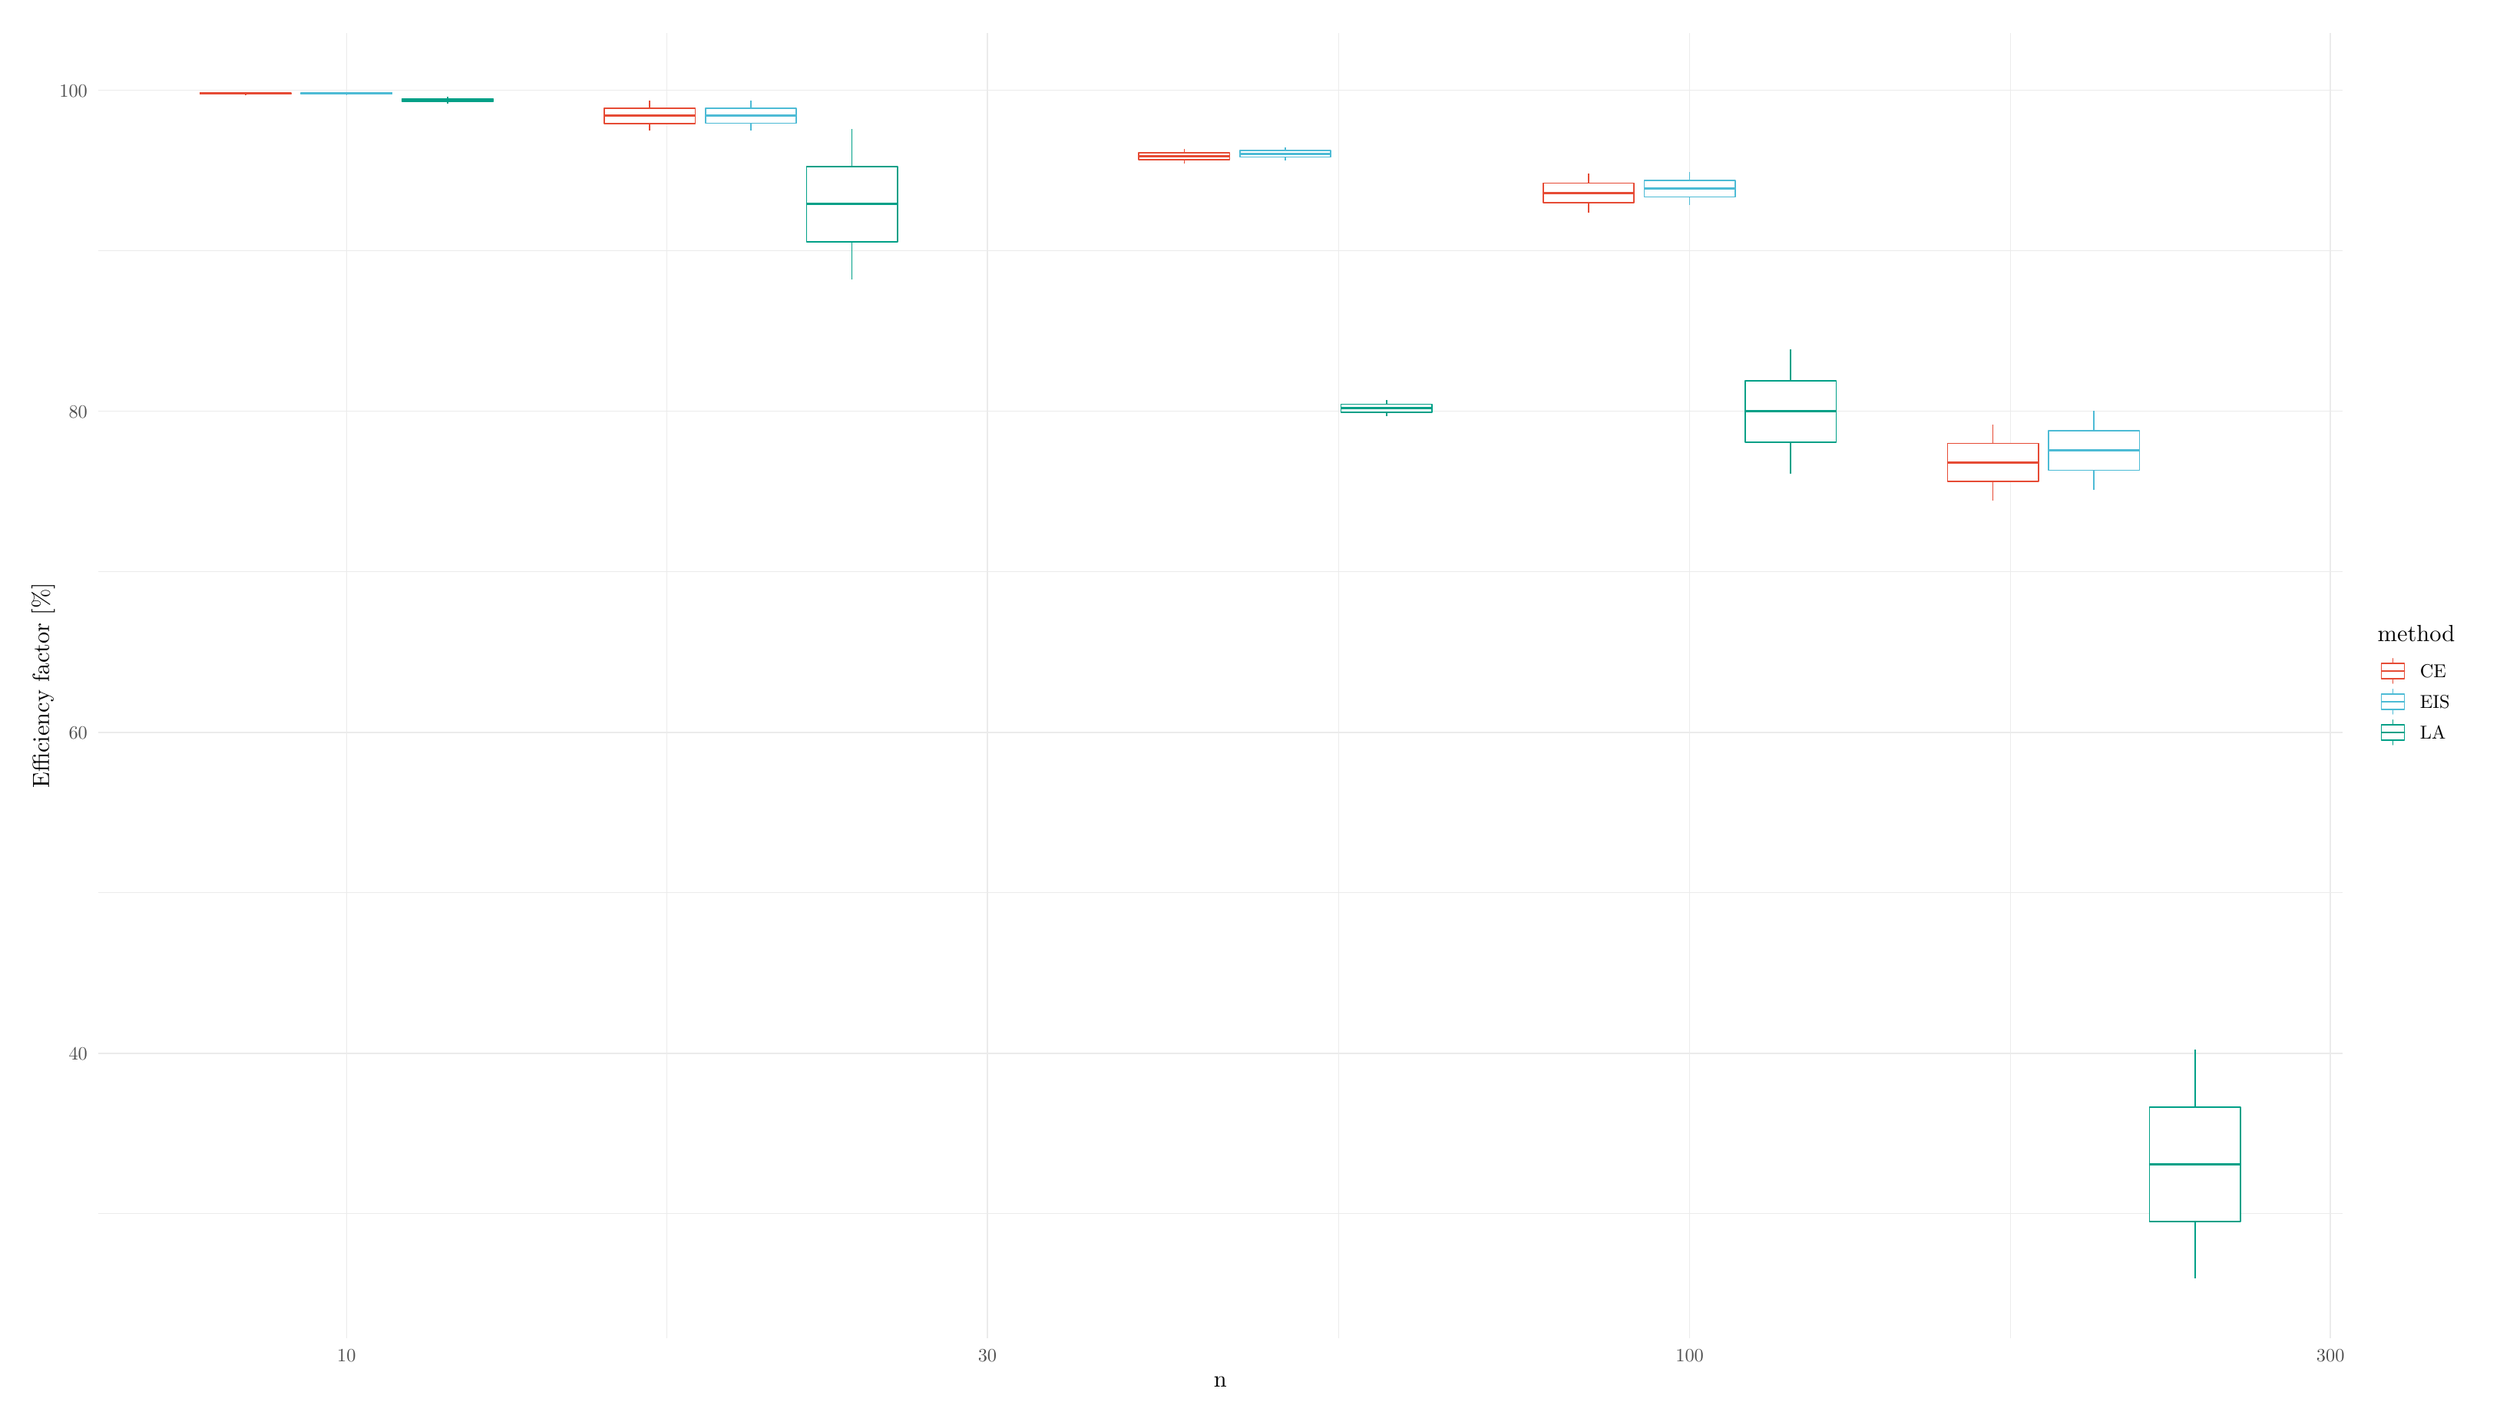
\begin{tikzpicture}[x=1pt,y=1pt]
\definecolor{fillColor}{RGB}{255,255,255}
\path[use as bounding box,fill=fillColor,fill opacity=0.00] (0,0) rectangle (1156.32,650.43);
\begin{scope}
\path[clip] ( 36.11, 30.69) rectangle (1092.47,644.93);
\definecolor{drawColor}{gray}{0.92}

\path[draw=drawColor,line width= 0.3pt,line join=round] ( 36.11, 89.19) --
	(1092.47, 89.19);

\path[draw=drawColor,line width= 0.3pt,line join=round] ( 36.11,240.26) --
	(1092.47,240.26);

\path[draw=drawColor,line width= 0.3pt,line join=round] ( 36.11,391.33) --
	(1092.47,391.33);

\path[draw=drawColor,line width= 0.3pt,line join=round] ( 36.11,542.40) --
	(1092.47,542.40);

\path[draw=drawColor,line width= 0.3pt,line join=round] (303.90, 30.69) --
	(303.90,644.93);

\path[draw=drawColor,line width= 0.3pt,line join=round] (619.94, 30.69) --
	(619.94,644.93);

\path[draw=drawColor,line width= 0.3pt,line join=round] (935.99, 30.69) --
	(935.99,644.93);

\path[draw=drawColor,line width= 0.6pt,line join=round] ( 36.11,164.72) --
	(1092.47,164.72);

\path[draw=drawColor,line width= 0.6pt,line join=round] ( 36.11,315.79) --
	(1092.47,315.79);

\path[draw=drawColor,line width= 0.6pt,line join=round] ( 36.11,466.86) --
	(1092.47,466.86);

\path[draw=drawColor,line width= 0.6pt,line join=round] ( 36.11,617.93) --
	(1092.47,617.93);

\path[draw=drawColor,line width= 0.6pt,line join=round] (153.10, 30.69) --
	(153.10,644.93);

\path[draw=drawColor,line width= 0.6pt,line join=round] (454.69, 30.69) --
	(454.69,644.93);

\path[draw=drawColor,line width= 0.6pt,line join=round] (785.20, 30.69) --
	(785.20,644.93);

\path[draw=drawColor,line width= 0.6pt,line join=round] (1086.78, 30.69) --
	(1086.78,644.93);
\definecolor{drawColor}{RGB}{230,75,53}

\path[draw=drawColor,line width= 0.6pt,line join=round] (105.53,616.69) -- (105.53,616.99);

\path[draw=drawColor,line width= 0.6pt,line join=round] (105.53,616.10) -- (105.53,615.80);
\definecolor{fillColor}{RGB}{255,255,255}

\path[draw=drawColor,line width= 0.6pt,line join=round,line cap=round,fill=fillColor] ( 84.13,616.69) --
	( 84.13,616.10) --
	(126.94,616.10) --
	(126.94,616.69) --
	( 84.13,616.69) --
	cycle;

\path[draw=drawColor,line width= 1.1pt,line join=round] ( 84.13,616.39) -- (126.94,616.39);

\path[draw=drawColor,line width= 0.6pt,line join=round] (295.81,609.43) -- (295.81,612.96);

\path[draw=drawColor,line width= 0.6pt,line join=round] (295.81,602.35) -- (295.81,598.82);

\path[draw=drawColor,line width= 0.6pt,line join=round,line cap=round,fill=fillColor] (274.41,609.43) --
	(274.41,602.35) --
	(317.22,602.35) --
	(317.22,609.43) --
	(274.41,609.43) --
	cycle;

\path[draw=drawColor,line width= 1.1pt,line join=round] (274.41,605.89) -- (317.22,605.89);

\path[draw=drawColor,line width= 0.6pt,line join=round] (547.35,588.56) -- (547.35,590.26);

\path[draw=drawColor,line width= 0.6pt,line join=round] (547.35,585.16) -- (547.35,583.46);

\path[draw=drawColor,line width= 0.6pt,line join=round,line cap=round,fill=fillColor] (525.94,588.56) --
	(525.94,585.16) --
	(568.75,585.16) --
	(568.75,588.56) --
	(525.94,588.56) --
	cycle;

\path[draw=drawColor,line width= 1.1pt,line join=round] (525.94,586.86) -- (568.75,586.86);

\path[draw=drawColor,line width= 0.6pt,line join=round] (737.63,574.25) -- (737.63,578.85);

\path[draw=drawColor,line width= 0.6pt,line join=round] (737.63,565.05) -- (737.63,560.45);

\path[draw=drawColor,line width= 0.6pt,line join=round,line cap=round,fill=fillColor] (716.22,574.25) --
	(716.22,565.05) --
	(759.03,565.05) --
	(759.03,574.25) --
	(716.22,574.25) --
	cycle;

\path[draw=drawColor,line width= 1.1pt,line join=round] (716.22,569.65) -- (759.03,569.65);

\path[draw=drawColor,line width= 0.6pt,line join=round] (927.91,451.78) -- (927.91,460.73);

\path[draw=drawColor,line width= 0.6pt,line join=round] (927.91,433.88) -- (927.91,424.94);

\path[draw=drawColor,line width= 0.6pt,line join=round,line cap=round,fill=fillColor] (906.50,451.78) --
	(906.50,433.88) --
	(949.31,433.88) --
	(949.31,451.78) --
	(906.50,451.78) --
	cycle;

\path[draw=drawColor,line width= 1.1pt,line join=round] (906.50,442.83) -- (949.31,442.83);
\definecolor{drawColor}{RGB}{77,187,213}

\path[draw=drawColor,line width= 0.6pt,line join=round] (153.10,616.72) -- (153.10,617.01);

\path[draw=drawColor,line width= 0.6pt,line join=round] (153.10,616.15) -- (153.10,615.86);

\path[draw=drawColor,line width= 0.6pt,line join=round,line cap=round,fill=fillColor] (131.70,616.72) --
	(131.70,616.15) --
	(174.51,616.15) --
	(174.51,616.72) --
	(131.70,616.72) --
	cycle;

\path[draw=drawColor,line width= 1.1pt,line join=round] (131.70,616.44) -- (174.51,616.44);

\path[draw=drawColor,line width= 0.6pt,line join=round] (343.38,609.50) -- (343.38,613.04);

\path[draw=drawColor,line width= 0.6pt,line join=round] (343.38,602.43) -- (343.38,598.90);

\path[draw=drawColor,line width= 0.6pt,line join=round,line cap=round,fill=fillColor] (321.98,609.50) --
	(321.98,602.43) --
	(364.79,602.43) --
	(364.79,609.50) --
	(321.98,609.50) --
	cycle;

\path[draw=drawColor,line width= 1.1pt,line join=round] (321.98,605.97) -- (364.79,605.97);

\path[draw=drawColor,line width= 0.6pt,line join=round] (594.92,589.52) -- (594.92,591.02);

\path[draw=drawColor,line width= 0.6pt,line join=round] (594.92,586.50) -- (594.92,584.99);

\path[draw=drawColor,line width= 0.6pt,line join=round,line cap=round,fill=fillColor] (573.51,589.52) --
	(573.51,586.50) --
	(616.32,586.50) --
	(616.32,589.52) --
	(573.51,589.52) --
	cycle;

\path[draw=drawColor,line width= 1.1pt,line join=round] (573.51,588.01) -- (616.32,588.01);

\path[draw=drawColor,line width= 0.6pt,line join=round] (785.20,575.56) -- (785.20,579.45);

\path[draw=drawColor,line width= 0.6pt,line join=round] (785.20,567.77) -- (785.20,563.88);

\path[draw=drawColor,line width= 0.6pt,line join=round,line cap=round,fill=fillColor] (763.79,575.56) --
	(763.79,567.77) --
	(806.60,567.77) --
	(806.60,575.56) --
	(763.79,575.56) --
	cycle;

\path[draw=drawColor,line width= 1.1pt,line join=round] (763.79,571.66) -- (806.60,571.66);

\path[draw=drawColor,line width= 0.6pt,line join=round] (975.48,457.70) -- (975.48,467.03);

\path[draw=drawColor,line width= 0.6pt,line join=round] (975.48,439.05) -- (975.48,429.72);

\path[draw=drawColor,line width= 0.6pt,line join=round,line cap=round,fill=fillColor] (954.07,457.70) --
	(954.07,439.05) --
	(996.88,439.05) --
	(996.88,457.70) --
	(954.07,457.70) --
	cycle;

\path[draw=drawColor,line width= 1.1pt,line join=round] (954.07,448.38) -- (996.88,448.38);
\definecolor{drawColor}{RGB}{0,160,135}

\path[draw=drawColor,line width= 0.6pt,line join=round] (200.67,614.00) -- (200.67,614.74);

\path[draw=drawColor,line width= 0.6pt,line join=round] (200.67,612.51) -- (200.67,611.77);

\path[draw=drawColor,line width= 0.6pt,line join=round,line cap=round,fill=fillColor] (179.27,614.00) --
	(179.27,612.51) --
	(222.08,612.51) --
	(222.08,614.00) --
	(179.27,614.00) --
	cycle;

\path[draw=drawColor,line width= 1.1pt,line join=round] (179.27,613.26) -- (222.08,613.26);

\path[draw=drawColor,line width= 0.6pt,line join=round] (390.95,582.03) -- (390.95,599.71);

\path[draw=drawColor,line width= 0.6pt,line join=round] (390.95,546.68) -- (390.95,529.00);

\path[draw=drawColor,line width= 0.6pt,line join=round,line cap=round,fill=fillColor] (369.55,582.03) --
	(369.55,546.68) --
	(412.36,546.68) --
	(412.36,582.03) --
	(369.55,582.03) --
	cycle;

\path[draw=drawColor,line width= 1.1pt,line join=round] (369.55,564.36) -- (412.36,564.36);

\path[draw=drawColor,line width= 0.6pt,line join=round] (642.49,470.16) -- (642.49,472.06);

\path[draw=drawColor,line width= 0.6pt,line join=round] (642.49,466.37) -- (642.49,464.48);

\path[draw=drawColor,line width= 0.6pt,line join=round,line cap=round,fill=fillColor] (621.08,470.16) --
	(621.08,466.37) --
	(663.89,466.37) --
	(663.89,470.16) --
	(621.08,470.16) --
	cycle;

\path[draw=drawColor,line width= 1.1pt,line join=round] (621.08,468.27) -- (663.89,468.27);

\path[draw=drawColor,line width= 0.6pt,line join=round] (832.77,481.29) -- (832.77,495.84);

\path[draw=drawColor,line width= 0.6pt,line join=round] (832.77,452.20) -- (832.77,437.65);

\path[draw=drawColor,line width= 0.6pt,line join=round,line cap=round,fill=fillColor] (811.36,481.29) --
	(811.36,452.20) --
	(854.17,452.20) --
	(854.17,481.29) --
	(811.36,481.29) --
	cycle;

\path[draw=drawColor,line width= 1.1pt,line join=round] (811.36,466.75) -- (854.17,466.75);

\path[draw=drawColor,line width= 0.6pt,line join=round] (1023.04,139.43) -- (1023.04,166.37);

\path[draw=drawColor,line width= 0.6pt,line join=round] (1023.04, 85.55) -- (1023.04, 58.61);

\path[draw=drawColor,line width= 0.6pt,line join=round,line cap=round,fill=fillColor] (1001.64,139.43) --
	(1001.64, 85.55) --
	(1044.45, 85.55) --
	(1044.45,139.43) --
	(1001.64,139.43) --
	cycle;

\path[draw=drawColor,line width= 1.1pt,line join=round] (1001.64,112.49) -- (1044.45,112.49);
\end{scope}
\begin{scope}
\path[clip] (  0.00,  0.00) rectangle (1156.32,650.43);
\definecolor{drawColor}{gray}{0.30}

\node[text=drawColor,anchor=base east,inner sep=0pt, outer sep=0pt, scale=  0.88] at ( 31.16,161.69) {40};

\node[text=drawColor,anchor=base east,inner sep=0pt, outer sep=0pt, scale=  0.88] at ( 31.16,312.76) {60};

\node[text=drawColor,anchor=base east,inner sep=0pt, outer sep=0pt, scale=  0.88] at ( 31.16,463.83) {80};

\node[text=drawColor,anchor=base east,inner sep=0pt, outer sep=0pt, scale=  0.88] at ( 31.16,614.90) {100};
\end{scope}
\begin{scope}
\path[clip] (  0.00,  0.00) rectangle (1156.32,650.43);
\definecolor{drawColor}{gray}{0.30}

\node[text=drawColor,anchor=base,inner sep=0pt, outer sep=0pt, scale=  0.88] at (153.10, 19.68) {10};

\node[text=drawColor,anchor=base,inner sep=0pt, outer sep=0pt, scale=  0.88] at (454.69, 19.68) {30};

\node[text=drawColor,anchor=base,inner sep=0pt, outer sep=0pt, scale=  0.88] at (785.20, 19.68) {100};

\node[text=drawColor,anchor=base,inner sep=0pt, outer sep=0pt, scale=  0.88] at (1086.78, 19.68) {300};
\end{scope}
\begin{scope}
\path[clip] (  0.00,  0.00) rectangle (1156.32,650.43);
\definecolor{drawColor}{RGB}{0,0,0}

\node[text=drawColor,anchor=base,inner sep=0pt, outer sep=0pt, scale=  1.10] at (564.29,  7.64) {n};
\end{scope}
\begin{scope}
\path[clip] (  0.00,  0.00) rectangle (1156.32,650.43);
\definecolor{drawColor}{RGB}{0,0,0}

\node[text=drawColor,rotate= 90.00,anchor=base,inner sep=0pt, outer sep=0pt, scale=  1.10] at ( 13.08,337.81) {Efficiency factor [\%]};
\end{scope}
\begin{scope}
\path[clip] (  0.00,  0.00) rectangle (1156.32,650.43);
\definecolor{drawColor}{RGB}{0,0,0}

\node[text=drawColor,anchor=base west,inner sep=0pt, outer sep=0pt, scale=  1.10] at (1108.97,358.45) {method};
\end{scope}
\begin{scope}
\path[clip] (  0.00,  0.00) rectangle (1156.32,650.43);
\definecolor{drawColor}{RGB}{230,75,53}

\path[draw=drawColor,line width= 0.6pt,line join=round,line cap=round] (1116.19,338.87) --
	(1116.19,341.04);

\path[draw=drawColor,line width= 0.6pt,line join=round,line cap=round] (1116.19,348.27) --
	(1116.19,350.44);
\definecolor{fillColor}{RGB}{255,255,255}

\path[draw=drawColor,line width= 0.6pt,line join=round,line cap=round,fill=fillColor] (1110.77,341.04) rectangle (1121.61,348.27);

\path[draw=drawColor,line width= 0.6pt,line join=round,line cap=round] (1110.77,344.65) --
	(1121.61,344.65);
\end{scope}
\begin{scope}
\path[clip] (  0.00,  0.00) rectangle (1156.32,650.43);
\definecolor{drawColor}{RGB}{77,187,213}

\path[draw=drawColor,line width= 0.6pt,line join=round,line cap=round] (1116.19,324.42) --
	(1116.19,326.59);

\path[draw=drawColor,line width= 0.6pt,line join=round,line cap=round] (1116.19,333.81) --
	(1116.19,335.98);
\definecolor{fillColor}{RGB}{255,255,255}

\path[draw=drawColor,line width= 0.6pt,line join=round,line cap=round,fill=fillColor] (1110.77,326.59) rectangle (1121.61,333.81);

\path[draw=drawColor,line width= 0.6pt,line join=round,line cap=round] (1110.77,330.20) --
	(1121.61,330.20);
\end{scope}
\begin{scope}
\path[clip] (  0.00,  0.00) rectangle (1156.32,650.43);
\definecolor{drawColor}{RGB}{0,160,135}

\path[draw=drawColor,line width= 0.6pt,line join=round,line cap=round] (1116.19,309.97) --
	(1116.19,312.13);

\path[draw=drawColor,line width= 0.6pt,line join=round,line cap=round] (1116.19,319.36) --
	(1116.19,321.53);
\definecolor{fillColor}{RGB}{255,255,255}

\path[draw=drawColor,line width= 0.6pt,line join=round,line cap=round,fill=fillColor] (1110.77,312.13) rectangle (1121.61,319.36);

\path[draw=drawColor,line width= 0.6pt,line join=round,line cap=round] (1110.77,315.75) --
	(1121.61,315.75);
\end{scope}
\begin{scope}
\path[clip] (  0.00,  0.00) rectangle (1156.32,650.43);
\definecolor{drawColor}{RGB}{0,0,0}

\node[text=drawColor,anchor=base west,inner sep=0pt, outer sep=0pt, scale=  0.88] at (1128.92,341.62) {CE};
\end{scope}
\begin{scope}
\path[clip] (  0.00,  0.00) rectangle (1156.32,650.43);
\definecolor{drawColor}{RGB}{0,0,0}

\node[text=drawColor,anchor=base west,inner sep=0pt, outer sep=0pt, scale=  0.88] at (1128.92,327.17) {EIS};
\end{scope}
\begin{scope}
\path[clip] (  0.00,  0.00) rectangle (1156.32,650.43);
\definecolor{drawColor}{RGB}{0,0,0}

\node[text=drawColor,anchor=base west,inner sep=0pt, outer sep=0pt, scale=  0.88] at (1128.92,312.72) {LA};
\end{scope}
\end{tikzpicture}
%
    }
    \caption{The efficiency factor degenerates as the number of time steps $n$ increases. We show the estimated efficiency factor over $100$ replications of estimating the optimal parameters for \Cref{ex:negbinom-ar1} with the \gls{cem} and \gls{eis} with $N_{\text{true}} = 10^{6}$ and the resulting estimated efficiency factors at the optimum. Notice the log scale of the x-axis. The performance of the optimal \gls{cem} and \gls{eis} parameters is comparable and superior to that of the \gls{la}}
    \label{fig:ef_time_dimension}
\end{figure}


\subsection{Breakdown of methods}

\subsection{Optimal parameters}

\begin{example}[Failure of \gls{la}]
  \label{ex:la_failure}
  Consider the Gaussian scale mixture $\P = \frac{1}{2} \left(\mathcal N (0,1) + \mathcal N(0, \varepsilon^{-2})\right)$ with mode $x^{\ast}=0$. 
  The \gls{la} is $\G_{\text{LA}} = \mathcal N \left( 0, \frac{1}{\varepsilon^{2} - \varepsilon + 1} \right)$, whose variance goes to $1$ as $\varepsilon$ goes to $0$, so the \gls{la} will miss close to $\frac 1 2$ of the total mass.
  For $\varepsilon$ small enough, the variance of the \gls{la} will be smaller than $\frac{1}{2\varepsilon^{2}}$, whence the second moment of the weights is infinite and importance sampling fails.

  The \gls{cem} minimizes the KL-divergence between $\P$ and $\G_{\psi}$, is given by $\G_{\text{CE}} = \mathcal N (0, \sigma^{2})$, where $\sigma^{2} = \frac{1}{2}\left( 1 + \varepsilon^{-2} \right)$ is the variance of $\P$.
  As $\sigma^{2} > \frac{1}{2}\varepsilon^{-2}$, the weights have finite second moment, and importance sampling is consistent.
  \todo{add proof for $\frac{1}{2}$ to appendix}
\end{example}

\subsection{Time complexity}

\subsection{Large sample behaviour}

\begin{itemize}
    \item stationary AR(1) process with high auto-correlation, NB observations, different $n$, large $N$, compare ESS, Variances, DKL(?)
\end{itemize}